\documentclass[a4paper,12pt]{jreport}
%---------------------------------------------------
\usepackage[dvipdfmx]{hyperref}
\usepackage{pxjahyper}
\usepackage{bm}
\usepackage{graphicx}
\usepackage{amssymb,amsmath}
\usepackage{ascmac}
\usepackage{float}
\usepackage{setspace}
\usepackage[dvipdfmx,usenames]{color}
\usepackage{colortbl}
\usepackage{algorithm}
\usepackage{algorithmic}
\usepackage{setspace}
\usepackage{subfigure}
\usepackage{here}
% \usepackage{redeffont}
\usepackage{listings,jvlisting} %日本語のコメントアウトをする場合jvlisting(もしくはjlisting)が必要
\usepackage{booktabs}
\usepackage{titlesec}
\usepackage{siunitx}
\usepackage{array}
\usepackage{multirow}
\usepackage[figure,table]{totalcount} 
%---------------------------------------------------
\definecolor{bl}{rgb}{0.94,0.97,1}
\definecolor{gr}{rgb}{0.5,0.5,0.5}
% \makeatletter
% \@removefromreset{figure}{chapter}
% \def\thefigure{\arabic{figure}}
% \makeatother
% \makeatletter
% \def\section{\newpage\@startsection {section}{1}{\z@}{2.3ex plus -1ex minus -.2ex}{2.3 ex plus .2ex}{\Large\bf}}
% \makeatother
%---------------------------------------------------
\setlength{\textwidth}{160truemm}
\setlength{\textheight}{240truemm}
\setlength{\topmargin}{-14.5truemm}
\setlength{\oddsidemargin}{-0.5truemm}
\setlength{\headheight}{0truemm}
\setlength{\parindent}{1zw}
\setlength{\parskip}{0cm} % 段落間
\setlength{\itemsep}{0cm} % 項目間
\setlength{\abovedisplayskip}{1pt}
\setlength{\belowdisplayskip}{1pt}
%---------------------------------------------------
\setstretch{1.0}
%---------------------------------------------------
\renewcommand{\subfigtopskip}{5pt}	% 図の上の隙間。上図の副題と下図の間。
\renewcommand{\subfigbottomskip}{0pt} % 図の下の隙間。副題と本題の間。
\renewcommand{\subfigcapskip}{-6pt}	% 図と副題の間
\renewcommand{\subcapsize}{\scriptsize} % 副題の文字の大きさ
\newcommand{\mysection}[1]{\vspace{-20pt}\section{#1}}
\newcommand{\mysubsection}[1]{\vspace{-20pt}\subsection{#1}}
\newcommand{\mysubsubsection}[1]{\vspace{-10pt}\subsubsection{#1}}
\renewcommand{\lstlistingname}{ソースコード}
\setcounter{tocdepth}{3}
\setcounter{secnumdepth}{3}
\renewcommand{\bibname}{参考文献}
\newcommand{\eqdef}{\overset{\rm{def}}{=}}
\newsavebox{\mybox}
%---------------------------------------------------
% ヘッダーとフッターの設定
\usepackage{fancyhdr}
\rhead{\leftmark}
\chead{}
\lhead{\rightmark}
\cfoot{\thepage}

\titleformat{\chapter}% command
    [display]% shape
    {\bfseries\gtfamily\LARGE}% format
    {第\thechapter 章}% label
    {0.5em}% sep
    {}% before-code

\rfoot{}
\begin{document}
%---------------------------------------------------
%ここからソースコードの表示に関する設定
\lstset{
  basicstyle={\ttfamily},
  identifierstyle={\small},
  commentstyle={\smallitshape},
  keywordstyle={\small\bfseries},
  ndkeywordstyle={\small},
  stringstyle={\small\ttfamily},
  frame={tb},
  breaklines=true,
  columns=[l]{fullflexible},
  numbers=left,
  xrightmargin=0zw,
  xleftmargin=3zw,
  numberstyle={\scriptsize},
  stepnumber=1,
  numbersep=1zw,
  lineskip=-0.5ex
}
%ここまでソースコードの表示に関する設定
%---------------------------------------------------
\vspace*{2cm}
\thispagestyle{empty}
\begin{spacing}{1}
\begin{center}
{\Large 明石工業高等専門学校専攻科 \\[1truecm]
専攻科特別研究論文} \\[3.5truecm]
\huge 遠隔型自動運転システムの \\
\huge ユーザビリティに関する研究 \\
\LARGE The Research of Usability of Remote and Autonomous Driving System\\[4truecm]
\Large ME2208 高橋 尚太郎 \\
(機械・電子システム工学専攻) \\[1truecm]
指導教員 野村 隼人
\end{center}
\pagenumbering{roman}
\tableofcontents
\end{spacing}

% 図がある場合のみ図目次を作成
\iftotalfigures
  \addcontentsline{toc}{chapter}{\listfigurename}  % 目次に図目次を追加
  \listoffigures  % 図目次を表示
\fi
% 表がある場合のみ表目次を作成
\iftotaltables
  \addcontentsline{toc}{chapter}{\listtablename}  % 目次に表目次を追加
  \listoftables  % 表目次を表示
\fi

\newpage
\clearpage
\pagenumbering{arabic}
\pagestyle{fancy}
\setlength{\headheight}{5truemm}


\chapter{序論}
\section{研究背景}

近年、様々な自律移動ロボットの研究開発が行われ、徐々に人間の生活環境に進出し始めている。
従来は、工場における産業用無人搬送車が主体であったが、活躍の場がオフィス、家庭、さらには屋外へと広がりつつある。
今後、ロボットを用いた省力化や危険な仕事の代替を進めるためには、自律移動ロボットが活動できる領域が人間の生活環境へと拡大していくことが期待される。

一例として、自律移動の応用技術として交通課題の解決策として自動運転システムの実用化が進んでいる。現在は法定上遠隔地からの監視・運用を必要とする遠隔型自動運転システムが想定されている。
遠隔型自動運転では、FPV(First Person View)における車速の制御に関して、ドライバの体感速度変化を促すための視覚効果に関する研究が行われている。
視覚効果は、定式化に関して未知数であり、体感速度変化の評価はドライバ自身の知覚の個人差を含めた主観で考えられるため、定性的解析に委ねられている。

自律移動ロボットの実現に関して、工場のように限定された環境では、環境をロボットのために整備することが可能であった。
しかしロボットの活動領域を広げるためには、環境をロボットに合わせて整備するのではなく、ロボットが様々な環境に適応することが求められる。
人間の生活環境は整備された工場と比較して複雑であり、不確実性が高くなる環境である。この不確実性への対処が、重要な課題となる。
特に、ロボットに必要となる知覚、計画、制御のうち、不確実性に最も深く関わるのが知覚(計測と認識)である。
移動ロボットを対象として考えると、重要な知覚の機能として自己位置推定と地図生成(SLAM: Simultaneous Localization and Mapping)がある。
自己位置推定は、ロボットが自身の位置(方位を含む)を認識しながら目的地まで移動するために必要となる。
また地図は、自己位置推定や経路計画に必要である。人手による地図の生成は多大な工数が必要なため、ロボットが自動的に生成することが望ましい。
移動ロボットの自己位置推定と地図生成において不確実性に対処するには、確率論に基づく手法が有効であることが知られている。
確率論に基づくことで、センサデータやコンピュータが持つモデルの不確実性を明示的に表現すると共に、事前確率の情報を用いてより確実性の高い推定を行うことが可能となる。
一般に、SLAMでは、外界センサであるLiDARに加えて、ロータリーエンコーダ、慣性測定ユニット(IMU)等の内界センサによるロボットの移動量の内部情報(オドメトリ)を用いることで、マッピングを行うことが主流とされているが、オドメトリを必要としない、オドメトリフリーのSLAM手法も提案されている。

自律移動ロボットの開発プロセスにおいて、実環境における実証実験が数多く行われている。
特に、屋外における自律移動においては、シミュレーションと実環境では、制約や環境条件が全く異なるため、実環境のみでしか得ることのできない知見が多く、自律移動の実用化に向けては、実機を用いた実証実験が必要とされている。
実証実験に代表されるつくばチャレンジでは、自律移動ロボットの設計において、要素技術であるLiDARを中心とした、センサ系の使用が主となり、複数のセンサとの融合(センサフュージョン)による環境認識の高精度化が図られている。
それと同時に、自律移動ロボットの実用化に向けて、使用されるセンサの選定、用途に応じて最適化する試みが行われている。
特に、ロボットに搭載するセンサの使用数を少なくすることは、ロボットに課される制約・条件、ソフトウェア開発の工数減、保守性の向上のために、考慮すべき点と述べられている。
自律移動チャレンジの参加車両の形態は多様であり、差動二輪型が一般的であるが、パーソナルビークル等の使用としては、4輪車両型の自律移動等も見られる。
自律移動ロボットは、歩行者等と同じ空間に共存するロボットとしての位置づけであり、比較的低速であることが特徴であり、LiDARによる環境認識の比重が高い。
対して、自動運転では、リアルタイム性が重視され、カメラや深度センサ等のイメージセンサ等のコンピュータビジョンとLiDARセンサによるSLAMがそれぞれ同じ割合での併用が標準となり、センサ融合に関する技術について言及されている。

\section{本研究の目的と特徴}
本研究では、ROS\verb|(Robot Operating System)|
を用いた4輪車両型自律移動ロボットシステムの開発を目的として、一つ目に、LiDARのみによるSLAMによって生成された環境地図の評価と、二つ目にステアリングコントローラによる、ハンドルフットペダル型インターフェースによる遠隔操作を用いた、手動運転自動運転の切り替えシステムの開発を行う。
ROSに実装されたSLAMメタパッケージである、
slam\_gmapping
による環境地図構築とNavigationメタパッケージである、Navigation Stack を用いて、Waypoint Navigationにより、中継目的地を経由して、
最終目的地まで自律移動を行い、最終目的地に到着した時点で、手動運転に切り替えることで、運転操作の引継ぎを実現するシステムを構築する。
三つ目に、遠隔型自動運転システムのFPV操作に着目した、自動車の映像における、運転視野角や、映像画角の変化による体感速度のモデルの定量化を目的として、体感速度モデルの定式化を提案する。
自律移動ロボットの要素技術として用いられているLiDARのメーカーとして有名な北陽電機株式会社は、中之島チャレンジに参加し、自律移動ロボットの実機を開発して、実際にフィールドで議論を行うことで、新製品の開発を行っている。
自律移動ロボットの要素技術であるLiDARの開発においても、実証実験が不可欠である。
筆者は、中之島ロボットチャレンジを観戦することで、将来的に自律移動ロボットやLiDARの開発に携わりたいと考えた。
今回は、縁あって北陽電機株式会社様よりLiDARを貸与頂き、有効活用して筆者自らの開発アイデアを実現することを目標として研究に取り組むこととした。
本研究の位置付けは、LiDARの使用技術の勉強並びに、北陽電機株式会社様への就職を目的としている。

\section{本論文の構成}

本論文は全5章から構成される。以下に各章の概要を述べる。

第1章では、本研究の背景と目的及び各章の構成を述べた。

第2章「FPV車両操作の体感速度変化率の定式化」では、ドライバの体感速度変化を促すための視覚効果に関する仮説を提案する。具体的には、体感速度の変化率を支配するパラメータに着目し、走行映像の視聴環境ドライバの視野角と、走行映像のクロップ率をパラメータとしたときの単位時間当たりの映像ピクセルの移動量を体感速度の変化率として、クロップ率・視野角の減少と増加の特性を一つのモデルとして定式化した。

第3章「LiDARのみのSLAMで作成された環境地図の評価」では、内界センサによるオドメトリを用いず、ROSで実装されている各LiDAR SLAMパッケージを用いたLiDARのみによる環境地図作成システムを開発し、オドメトリフリーの手法に対して、オドメトリが必要な手法にLiDARから得るレーザオドメトリを用いて比較することで、LiDARのみによるSLAMの性能を明らかにした。

第4章「自動運転システムの開発」では、測距センサ(LiDAR)による測距データのみを用いたSLAMによって作成された環境地図を用いて、4輪車両型RCカーのLiDARのみによる自己位置推定とWaypoint Navigationの有用性の検証を行った。特に、4輪車両特有の動作である、切り返しの実現性、自動運転システムとして機能をする場合の遠隔操作のユーザビリティと、手動・自動運転のタスクの切り替え機能の動作に着目をした評価を行った。

第5章「結論」では、本研究で得られた結果とその成果について述べる。


\chapter{FPV車両操作の体感速度変化率の定式化}
\section{はじめに}
体感速度の変化とは、基準となる速度に対して、観測環境における何らかのパラメータの作用により、視覚的な体感情報から得られる速度感覚が基準と比べて変化する現象のことである。
自動車を運転する際、車速の増加によってドライバの有効視野角が狭まり、ドライバの体感速度が減少する現象が報告されている。
また、低速状態においても、ドライバの視野角の変化、運転視野映像のクロップによって体感速度が変化する現象が一般的に知られている。
また、自動車等を、カメラ映像を確認しながら遠隔操作(FPV:First Person View操作)する際に、カメラの設定によって同様の現象が起こる。
これはカメラ映像による視覚情報が、遠隔操作を行うための操作者への体感情報に影響を与えるためだと考えられている。
具体的には、カメラの画角の設定などが挙げられる。FPVは、操作対象から見た視点であり、操作者が操作対象から周囲の景色を見ることを目的としている。
自動車の運転操作と、遠隔型自動運転や、FPVによるRCカーの操作では、スケールの違いや、カメラの画角の設定等から、視覚情報から得られる体感情報において矛盾が生じる。
一例として、操作対象自身の視点から体感する感覚的な移動速度(体感速度)を錯覚する。
一般に、自動車のドライバが利用する情報のおよそ 90\%が 視覚情報であると報告されており、ドライバが受け取る情報の大部分を占めているため、体感速度の錯覚が、適切な運転に影響を与え、思わぬ事故を引き起こす恐れがある。
体感速度の錯覚は、走行環境と自動車の運転速度の変化によっても生じる。より広い道路を高速で移動すると、人間の視野における周辺視の減少により、自動車の体感速度を実際の速度よりも低く感じるように錯覚すると報告されている。
高速道路等で体感速度を低く感じると、ドライバは、車速を増加させる傾向にある。車速の増加が自動者事故の原因になる。
また、逆に低速域においても視野角の減少によって体感速度が減少することが報告されている。また、ゲーム等の演出で使用されているものとしては、視野を広げると速く見せることができる。
一方、運転映像や運転中の視野角の変化による体感速度の比率の定量化に関しては行われていない。視野角を狭めることによる効果や、視野の増加によって得られる体感速度の定量化\verb|(モデル化)|はされていない。
また、視野角の減少と増加の両方における体感速度の変化を一つの特性として表した例はない。
体感速度を定式化することができれば、映像から得られる視覚効果の影響を光学的に応用し、FPV操作や、ヘッドアップディスプレイ等によって、ドライバの体感情報の補正手法としての応用が期待できる。
そこで我々は、自動車の映像における体感速度のモデルの定量化を目的として、体感速度モデルの定式化を提案する。
DSの走行映像において観測者の体感速度の減少を促す映像クロップと視野角の特性を求め、クロップ率-体感速度と、視野角-体感速度の幾何学モデルを定式化する。
本研究では、クロップ率・視野角の減少と増加の特性を一つのモデルとして表し、視野角の変化に対する体感速度の変化を定式化することで、映像から得られる体感速度を定量的に定義した。

\section{従来研究}
淺田ら\cite{taikan:asada}は、人間の視覚情報を用いた体感速度変化を利用した研究として、ドライビングシミュレータの操作視点にバーチャルパターンを投影することによって、ドライバに適切な速度制御を促す手法が提案されている。
運転者の速度制御をモデル化することにより、ドライバが適切な速度を制御できない要因として「環境からの速度認知に関する誤差が大きいこと」、「目標速度設定が適切でないこと」の2点が挙げられることを明らかにした。
前者の要因を改善するバーチャルパターンとして、一定速度で移動するバーチャルパターン、流れる風景を誇張表現するバーチャルパターンを挙げ、バーチャルパターン投影映像の視聴実験の被験者の主観評価により、これらの有効性を確認した。
これらは、目標速度制御のための定性的な効果であり、体感速度の変化に寄与するパラメータについては言及されておらず、体感速度の変化を示すものは、被験者の主観による評価であるため、視覚効果の定量的な評価はされていない。

大前ら\cite{taikan:ohmae}は、遠隔操縦に基づく資格情報の影響を評価し、遠隔操縦において、カメラ条件や映像条件が運転操作に与える影響を評価している。評価結果に基づいて遠隔操縦車両および、その制御系を構築し、遠隔操縦と直接運転を比較することで、本研究で構築した遠隔操縦システムの構成により、直接運転と近い運転操作が実現できることを明らかにした。
視覚情報の影響評価においては、カメラの視野角の影響が大きく、フレームレートや解像度などの影響が相対的に小さいことが報告されている。
以上より、遠隔操縦における視覚情報の運転への影響として、視野角による影響が大きいことが述べられている。

Speed Management \cite{taikan:speedmanagement}によると、速度が上がるとドライバの視野が狭くなることが報告されている。
時速40 km の場合、ドライバの視野は 100度であり、路傍の障害物やその他の潜在的な危険を確認できる。図\ref{taikan:speed}に視野角と体感速度の関係を示す。
時速 130 km では、視野は約 30°にまで減少し、ドライバが潜在的な危険を判断する能力が大幅に低下するとされている。

\begin{figure}[h]
  \begin{center}
  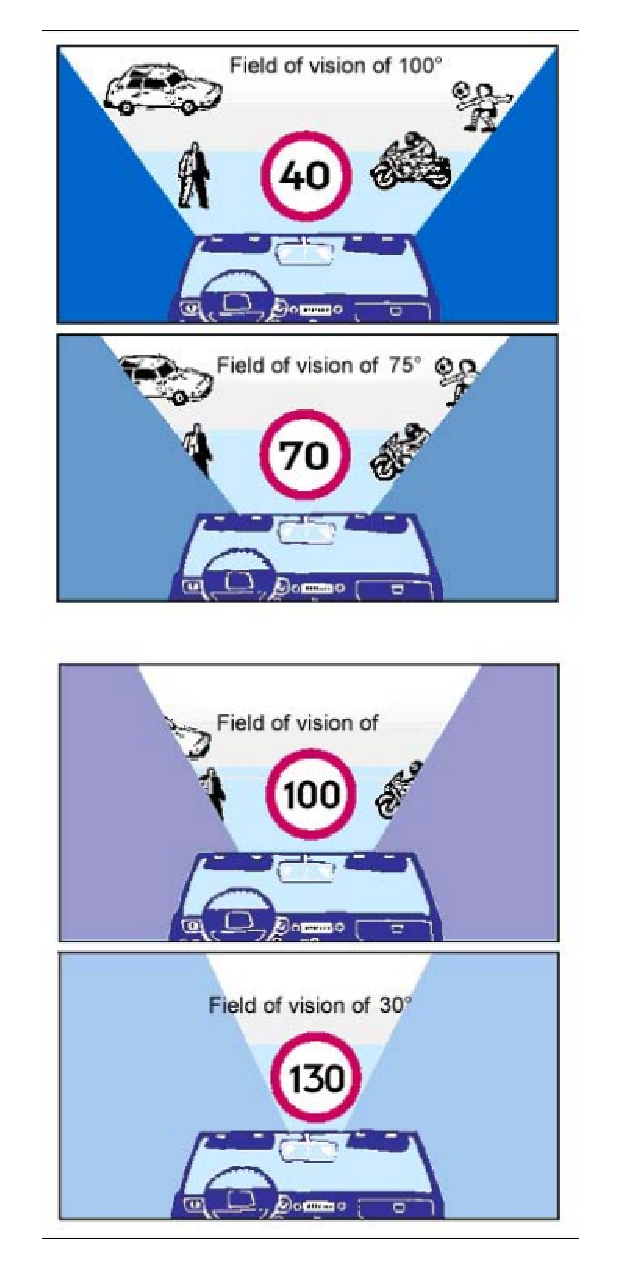
\includegraphics[width=.5\linewidth]{img/1.eps}
  \caption{視野角と体感速度の関係\cite{taikan:speedmanagement}}
  \label{taikan:speed}
  \end{center}
\end{figure}

\clearpage
体感速度を支配するパラメータとして、運転者の速度に影響を与えるパラメータに関する研究をいくつか述べる。

AR 技術を用いて運転者の体感速度を変化させる試みとして東井ら\cite{taikan:higashii}は単純な線や四角形からなるパターン の速度を実際よりも速く表示することで運転者の体感速度を変化させることに成功していた。しかし、実際にどのような速度制御が行われるかや他の表示方法で表示した場合の効果は未知数である。

走行速度と道路環境の関係についての調査として Gitelman\cite{taikan:gitelman}らは運転者が速度超過する原因は道路環境から人々が適切と感じる速度と制限速度があっていないこととし, どういった要素が適切と感じる速度に影響を与えているかを実際の道路環境の要素の調査と運転者への意識調査によって検証した。結果として視野的狭窄や歩行者の活動、道路のレイアウト等が要素として挙げられることが分かった。

Joら\cite{taikan:jo}は、運転速度がドライバの視覚的注意に及ぼす影響を、ドライバが処理できる視覚情報の最大量とのバランスがとれる最大視野という観点から評価を行った。
運転速度の増加により、処理する視覚情報の量が増加するため、ドライバが処理する視覚情報の量が、自身の取得できる最大量と釣り合う点までしか視野を広げることができないとした。
この点を超えるとドライバは、不安、ストレスの増加によりドライバが取得できる最大の視覚情報が減少し、視野がさらに狭くなって心理的圧迫感を感じる現象(トンネル効果)が起きる可能性があると述べている。具体的に、ドライバは、潜在的な危険があった場合に対処するための時間を確保するために、運転速度が上がるにつれて遠くを見る傾向がある。 これは、運転速度の増加による流体刺激の増加だけでなく、遠くを見ることでの視野の増加により、ドライバが処理する視覚情報の量が増加し、ドライバの精神的負担が増大することを意味する。ドライバは、安全を確保するために、取り扱える視覚情報の量が許される限り、可能な限り多くの視覚情報を取得する傾向にある。しかしながら、前述したように、運転者が取り込める最大の視覚情報は、運転の専門知識のレベルに応じて個人差がある。走行速度が取り込める視覚情報の許容量が釣り合う点を超えた場合、ドライバは自動的に視野を狭めることで視覚的情報の許容が釣り合う点を自己維持しようとし、処理する視覚情報の量を減らす。
一部のドライバにとっては、バランス点を超える不安ストレスが非常に高くなり、バランス点を超えた後に処理できる最大の視覚情報がさらに減少するとしている。

\section{体感速度のパラメータの模索}
RCカーと実車の速度が視覚的に一致すること(体感速度が一致すること)を目的として、体感速度の変化を及ぼすパラメータを、RCカー・DSの走行映像の比較により調査した。体感速度の比較について、車両模型の迫力・臨場感の表現として用いられるスケールスピードとの比較も行った。これにより体感速度の一致の目標が、走行映像中における単位時間当たりの描画の移動ピクセル数の一致であることが分かった。また、この目標を達成するためのパラメータを明らかにした。

\subsection{原理}
図\ref{taikan:genri}に、体感速度の原理を示す。
一般に、トラックなど乗用車よりも車高が高くなる車両を運転する場合、体感速度は遅くなり、
逆に、レースカート等の車高の低い車両を運転すると体感速度は速く感じる。RCカーを運転する場合は後者に相当する。その原理を幾何学的に説明する。

\begin{figure}[h]
  \begin{center}
  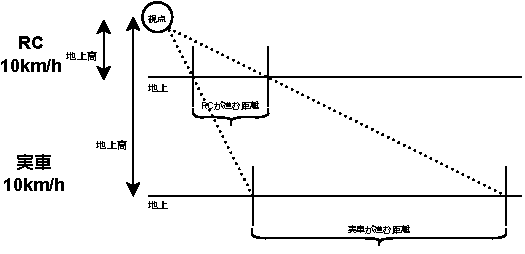
\includegraphics[width=.95\linewidth]{img/2.pdf}
  \caption{体感速度の原理}
  \label{taikan:genri}
  \end{center}
\end{figure}

体感速度の変化は上下・左右方向の視野それぞれの影響が存在する。
一例として上下方向の視野の場合を説明する。操作視点が高い時の視点は、低い時の視点の延長線上にある。
ある点から他方の点まで進んだ時も同様になる。実車あるいはRCカーが、体感的と同じ速度で移動しているための条件は、画面上のピクセルの移動速度(実際の線を移動する時間)が、実車とRCカーで同じになることである。
RCカーと実車で速度が同じでも、風景が移動する速度が異なるために体感速度が異なる。
このRCカーの実速度に対して体感速度が同じになる実車の速度との比を求めることで、体感速度の一致を求めることができる。
つまり、体感速度の一致を走行映像中の単位時間当たりの移動ピクセル数の一致とする。

\subsubsection{体感速度とスケールスピードについて}
スケールスピードとは、模型車両の実際の移動速度にスケール比の平方根を乗じたものを、実際の車両のスケールでの速度としたものである。
実際の速度にスケール比を乗ずるのではなく、力学的な相似効果から迫力の表現として使用されている。
スケールスピードの導出には、流体分野における流れの相似の指標とするフルード数が用いられ、以下のようにして導出する。

フルード数$Fr$の定義は、式\eqref{taikan:eq:frude}で表される。

\begin{align}
  Fr = \frac{U}{\sqrt{Lg}} \label{taikan:eq:frude}
\end{align}

ここで、$U$:体感速度\si{[m/s]}、$L$:代表長さ\si{[m]}、$g$:重力加速度\si{[m/s^2]}である。実車の特性速度、代表長さをそれぞれ、
$U_1$、$L_1$、RCカーの特性速度、代表長さを$U_2$、$L_2$とすると、それぞれが力学的に相似であることから、フルード数が一致するという条件のもとで、
立式すると式\eqref{taikan:eq:frude2}、\eqref{taikan:eq:frude3}のようになる。

\begin{align}
  \frac{U_1}{\sqrt{L_1g}} = \frac{U_2}{\sqrt{L_2g}} \label{taikan:eq:frude2}\\
  U_2 = \frac{U_1}{\sqrt{\frac{L_1}{L_2}}} \label{taikan:eq:frude3}
\end{align}

$\frac{L_1}{L_2}$は、実車とRCカーのスケール比であるため、特性速度、$U_2$がRCカーのスケールスピードであり、実車の速度$U_1$をスケール比の平方根で除すると求めることができる。

\subsection{DS・RCカーの走行映像の解析}
ここでは、DSとRCカーの走行映像の比較について述べる。
DS上の実速度とRCカーのスケールスピードが一致する場合RCカーと実車の体感速度が等しいと仮定して、
RCカーとDSの走行映像の単位時間あたりの移動ピクセル数の一致を目指す。またスケールスピードではなく、スケール比を乗じた速度での走行映像との比較も行った。

\subsubsection{実験方法}
\begin{enumerate}
  \item RCカーの走行環境を作成する。図\ref{taikan:rc}に、RCカーの走行環境を示す。今回は移動ピクセル数の比較のために、コース車両の脚部分に黄色い装飾を施した。RCカーに設置したカメラで定速走行映像を撮影し、始点・終点間の動画の再生時間で除して実速度を求め、スケール比の平方根との積によりスケールスピードを計算する。RCカーの移動速度は、RCカーのDCモータのPWM制御によって行われているため、PWM周期の入力値と出力値を実測する。この出力値を用いてRCカーの移動速度を計算している。
  \item DS上で実車スケールのRCカーの走行環境を作成する。図\ref{taikan:ds}にDS上で再現したRCカーの走行環境を示す。RCカーの現物の環境と視覚的な条件を等しくするために、RCカーの走行実験で使用した環境の壁面\verb|(机)|の寸法を測定し、走行路面をテクスチャマッピングによって再現した。
  \begin{figure}[h]
    \begin{center}
    \subfigure[RCカーの走行環境]{
    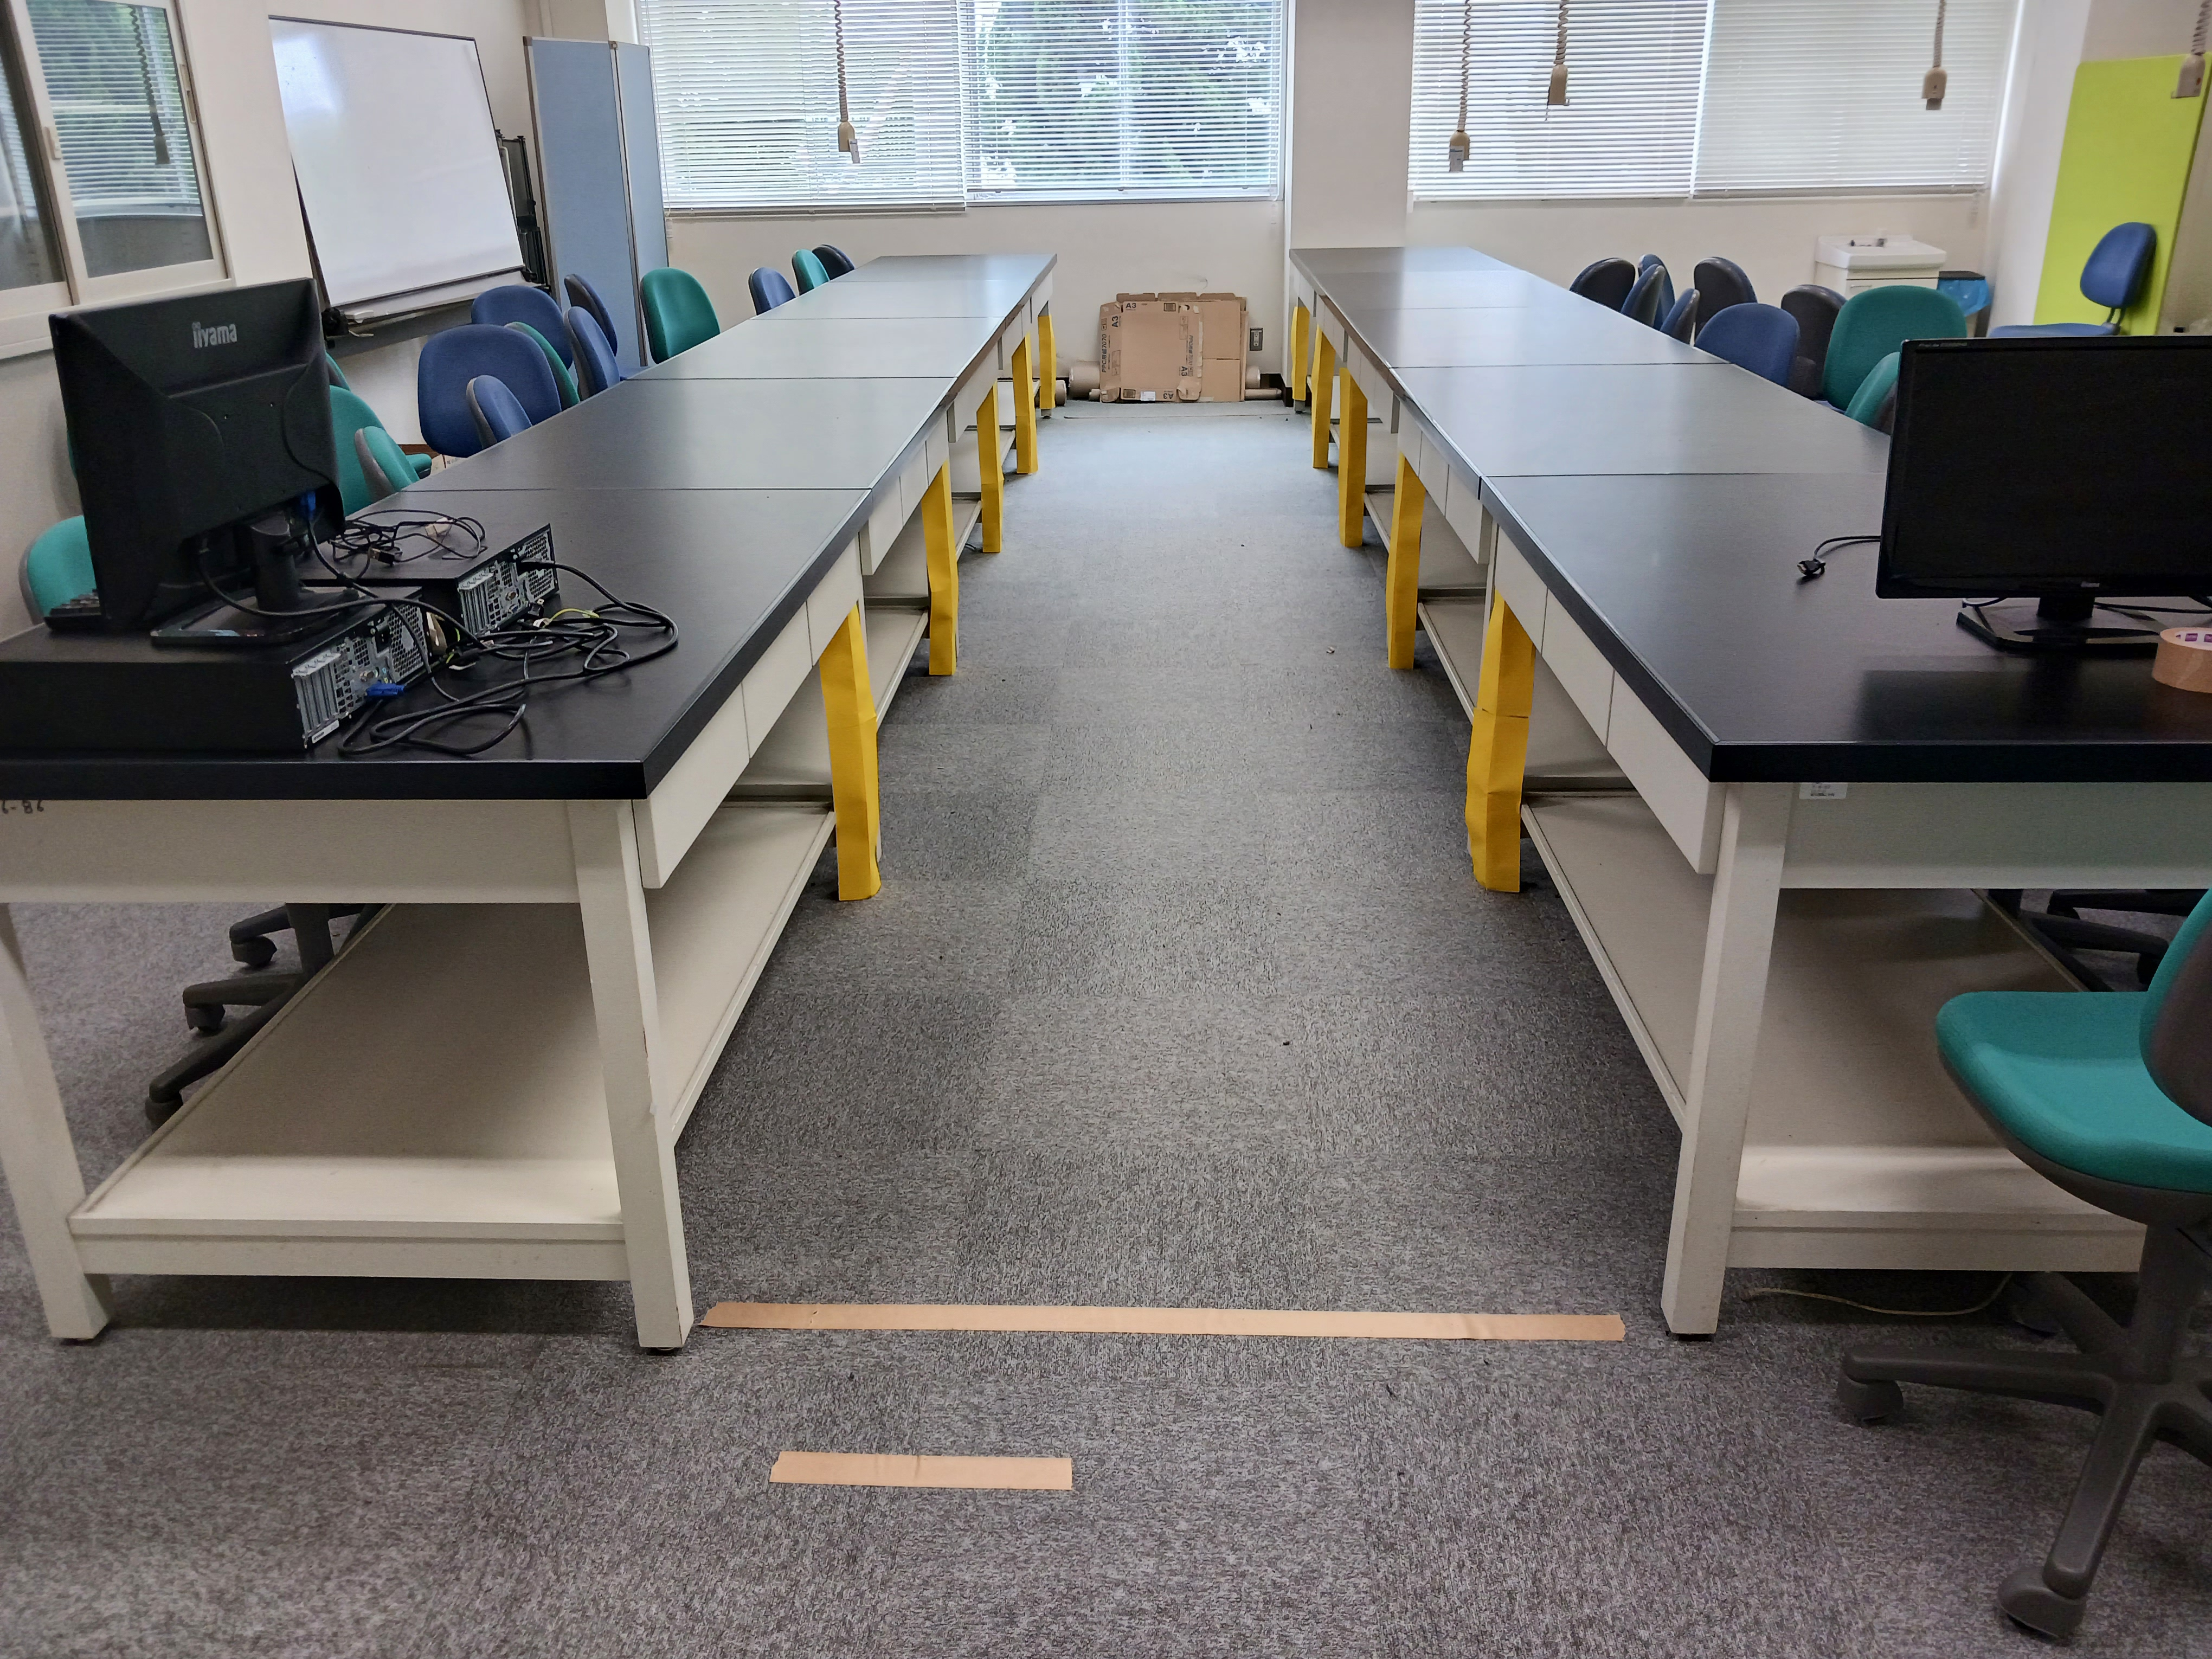
\includegraphics[width=.4\columnwidth]{img/3.jpg}
    \label{taikan:rc}
    }
    \subfigure[DS上で再現したRCカーの走行環境]{
    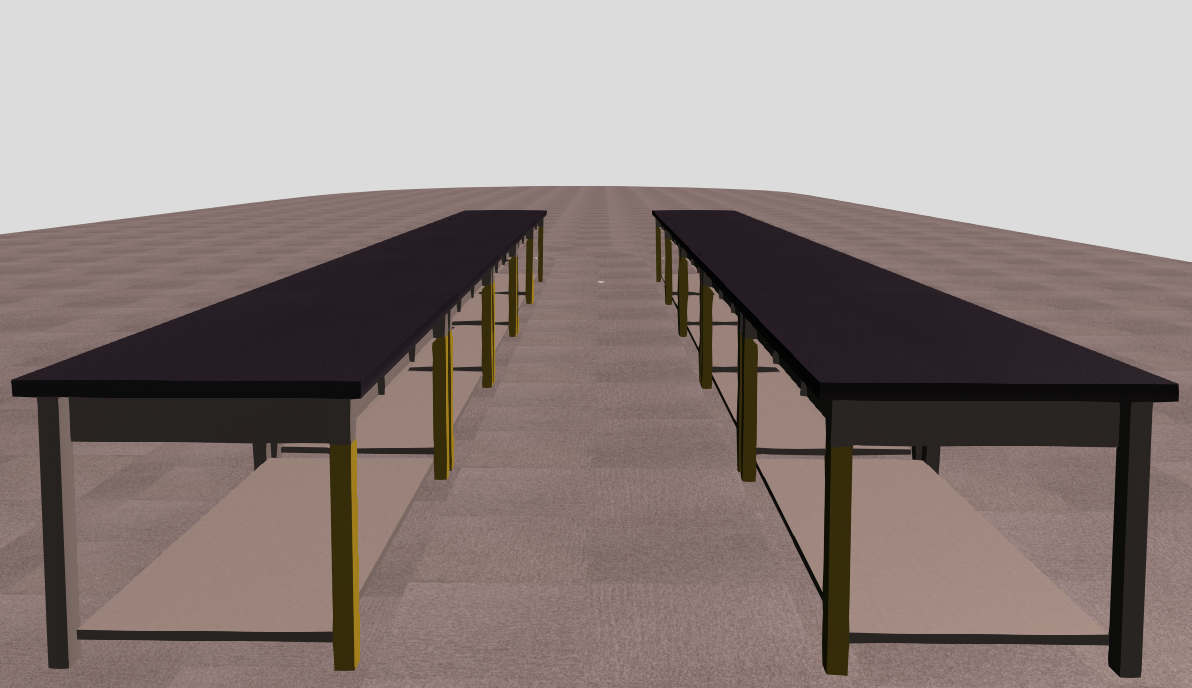
\includegraphics[width=.52\columnwidth]{img/4.png}
    \label{taikan:ds}
    }
    \caption{体感速度の実験環境}
    \label{taikan:jikken1}
    \end{center}
  \end{figure}
  \item DSの走行環境においてRCカーのスケールスピードで走行した映像を撮影する。DSとRCカーの走行映像を見比べて、単位時間当たりに通過するポールの数を目視で確認し、スケールスピードと体感速度の一致・不一致を評価する。
  \begin{figure}[h]
    \begin{center}
    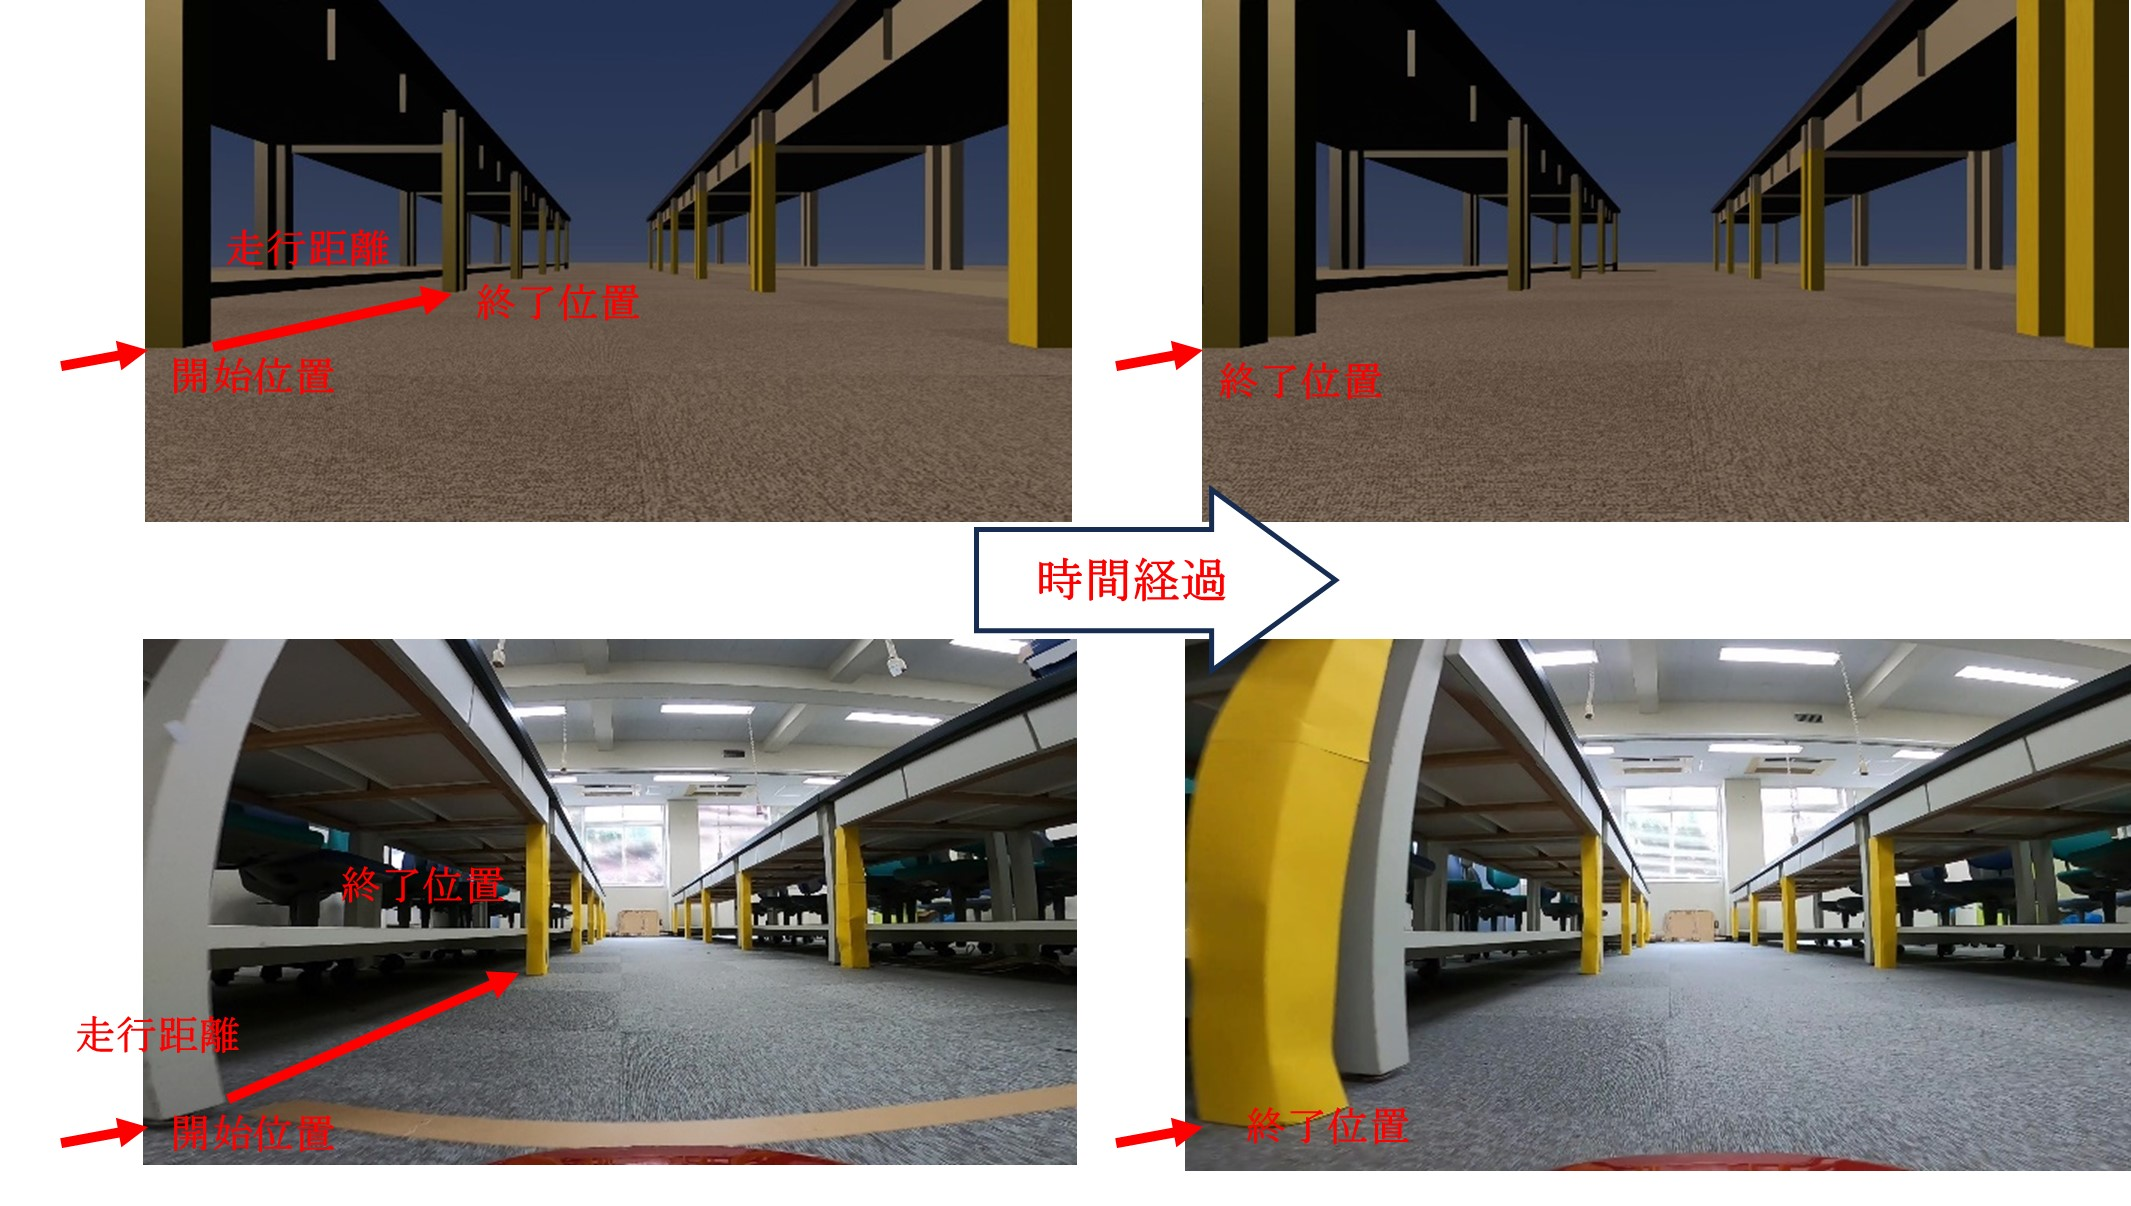
\includegraphics[width=.88\linewidth]{img/5.jpg}
    \caption{単位時間当たりに通過するポールの数の確認}
    \label{taikan:pall}
    \end{center}
  \end{figure}
  \item RC映像にスケール比を乗じた速度のRCカーの走行映像を取得する。
  \item スケールスピードでの比較とスケール比をかけた速度を比較する。
  \item 体感速度が一致しない場合、その原因を検討し、パラメータとする。
\end{enumerate}
なお、本実験で作成したDS環境の寸法を図\ref{taikan:dsm1}、\ref{taikan:dsm2}に示す。DS上の環境に関しては、RCカーのスケール比に合わせて作成した。
今回用いたRCカーのスケールが$\frac{1}{10}$であったため、実際のRCカーの走行環境を10倍したDS上の走行環境とした。

\begin{figure}[h]
  \begin{center}
  \subfigure[DS上コースの寸法:全体]{
  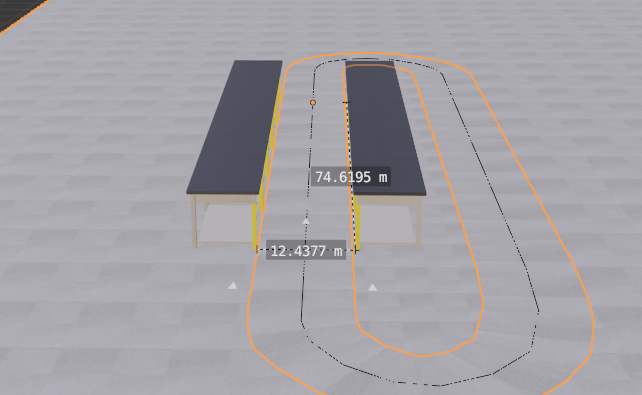
\includegraphics[width=.8\columnwidth]{img/6.png}
  \label{taikan:dsm1_1}
  }
  \subfigure[DS上コースの寸法:全長]{
  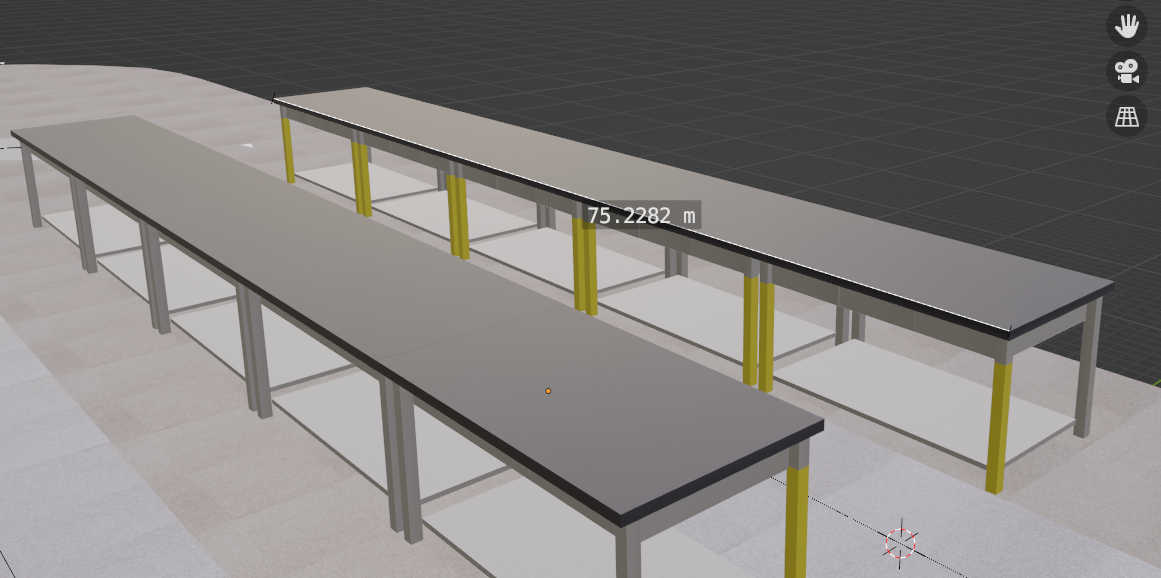
\includegraphics[width=.8\columnwidth]{img/7.png}
  \label{taikan:dsm1_2}
  }
  \caption{DS環境の寸法:全体}
  \label{taikan:dsm1}
  \end{center}
\end{figure}

\begin{figure}[h]
  \begin{center}
  \subfigure[DS上コースの寸法:障害物]{
  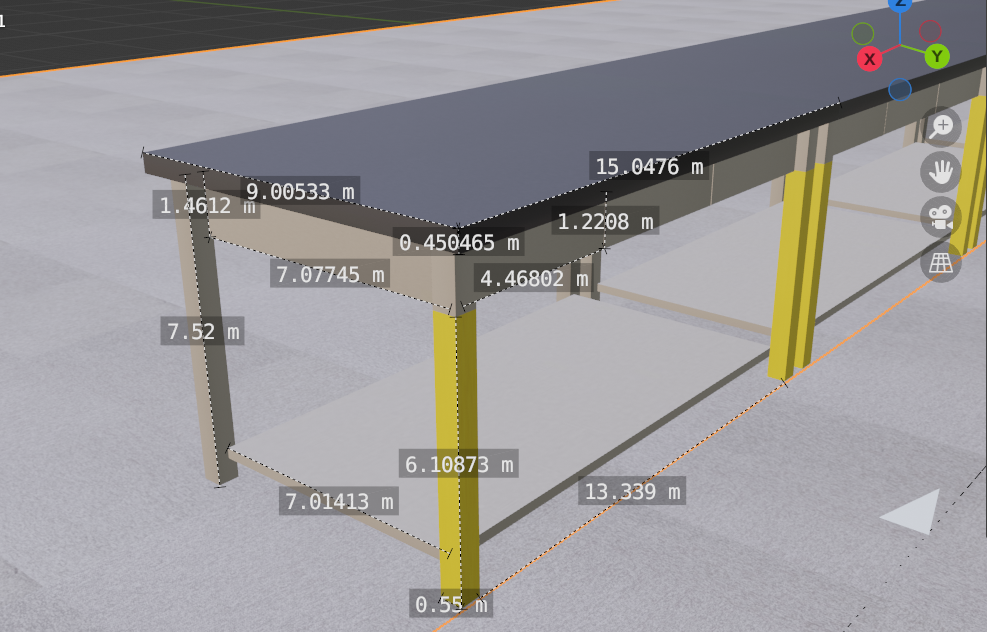
\includegraphics[width=.8\columnwidth]{img/8.png}
  \label{taikan:dsm2_1}
  }
  \subfigure[DS上コースの寸法:道幅]{
  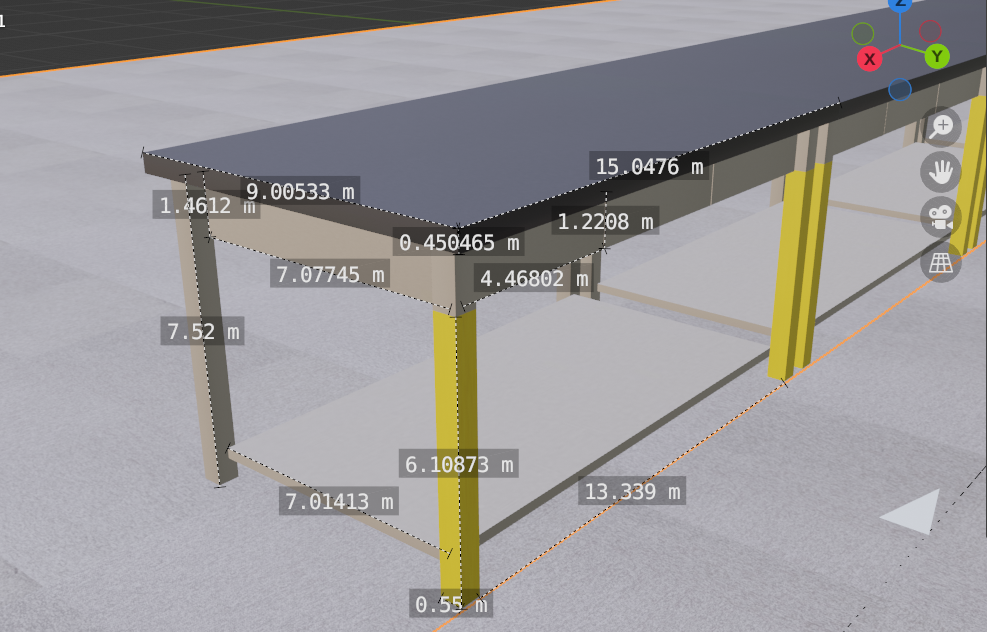
\includegraphics[width=.8\columnwidth]{img/8.png}
  \label{taikan:dsm2_2}
  }
  \caption{DS環境の寸法:詳細}
  \label{taikan:dsm2}
  \end{center}
\end{figure}

実験の様子を図\ref{taikan:hikaku}に示す。
今回のスケールスピードの比較は、表に示す32\verb|~|48 \si{[km/h]}
の6パターンで行った。一例として、RCカーのスケールスピード32 \si{[km/h]}(実際の速度は10\si{[km/h]})とDS上の速度32\si{[km/h]}の比較を行う。

スケール比での比較は、RCカー の実際の速度10 \si{[km/h]}とDSの100 \si{[km/h]}の映像で行った。
体感速度の評価を目的としてDSとRCカーの走行映像をPCディスプレイ上に並べて視聴する。
視聴者の主観によって体感速度の遅速・一致を評価する。体感速度が一致しない映像を観察することで、体感速度の変化を示すパラメータを模索する。

\begin{figure}[h]
  \begin{center}
  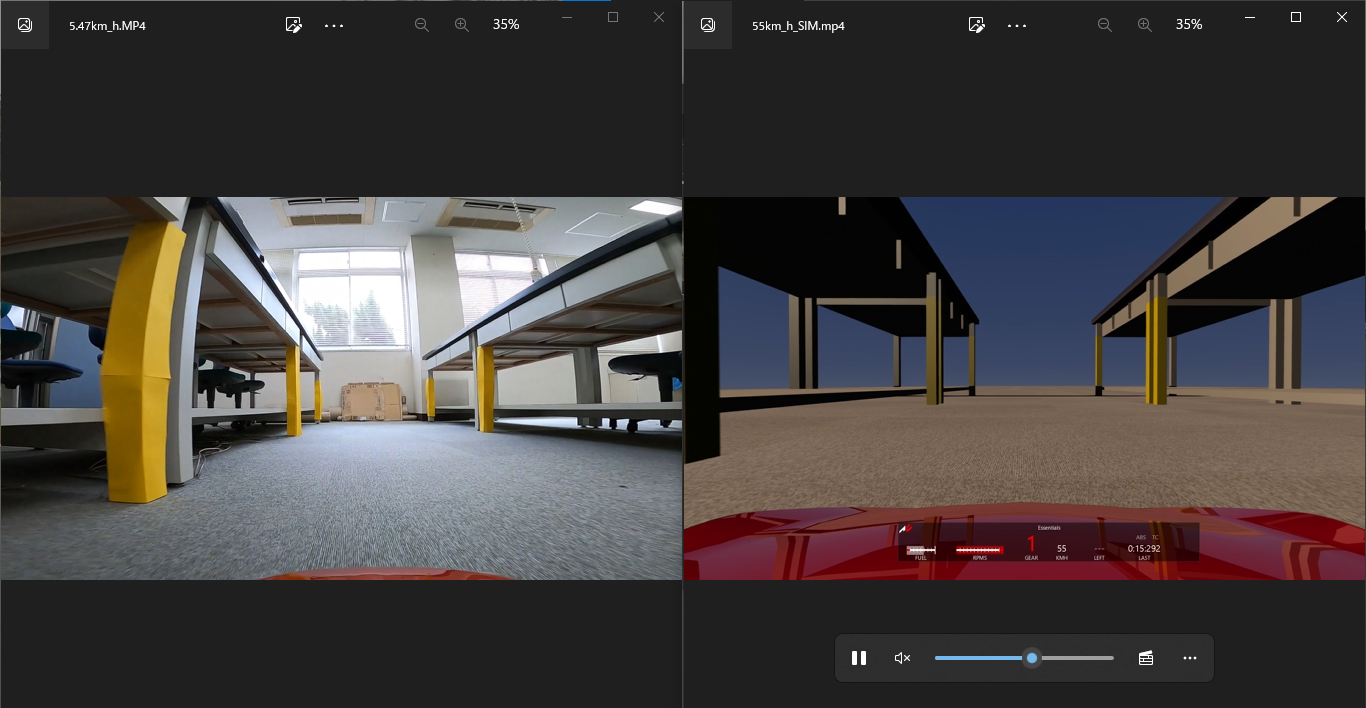
\includegraphics[width=\linewidth]{img/10.png}
  \caption{実験の様子}
  \label{taikan:hikaku}
  \end{center}
\end{figure}

\clearpage
\subsubsection{実験結果}
実測値とスケールスピードの計算結果を表\ref{taikan:table1}に示す。RCカーのスピードはモータの回転数を回転数計で計測し、
計算を行って、時速への変換を行っている。なお、モータの回転数は10回計測した際の平均値を採用している。
 
\begin{table}[ht]
\centering
\caption{実速度とスケールスピードの計算結果}
\scalebox{.83}{
\begin{tabular}[t]{rrrrrr}
\toprule
パルス入力値\si{[\micro s]}&パルス測定値\si{[\micro s]}&パルス誤差&回転数\si{[rpm]}&実速度\si{[km/h]}&スケールスピード\si{[km/h]}\\
\midrule
1348&1329&19&2194&24.81&78.47\\
1402&1386&16&1896&21.44&67.81\\
1438&1418&20&1589&17.97&56.83\\
1458&1440&18&1337&15.12&47.82\\
1480&1460&20&1161&13.13&41.52\\
1502&1482&20&854.6&9.666&30.57\\
\bottomrule
\label{taikan:table1}
\end{tabular}}
\end{table}%

モータの回転数を時速に変換する式を式\eqref{taikan:eq:motor}に示す。
\begin{align}
  v_{km} = d \times r \times 0.01885 \label{taikan:eq:motor}
\end{align}
ここで、$v_{km}$:時速、$d$:ホイールの直径\verb|(|6 \si{[cm]}\verb|)|、$r$:回転数\si{[rpm]}、\\0.001885:係数成分:$\frac{3600}{1000}\times\frac{2\pi}{60\times100}$
である。

RCカーのスケールスピード32 \si{[km/h]}\verb|(|実際の速度は10 \si{[km]}\verb|)|とDS上の速度32 \si{[km/h]}で比較した場合は、体感速度が一致しなかった。RCカーの速度10 \si{[km/h]}とDS上の速度100 \si{[km/h]}を比較した場合は、体感速度が一致した。
実験結果より、RCカーの操作視点カメラ映像の方が、DSの操作映像よりも体感速度が速いと評価されるため、RCカーのスケールスピードは体感速度と一致しないことを確認した。また、スケール比で走行させた場合に体感速度が一致したことから、
RCカーと自動車における移動ピクセル比は、スケール比の平方根ではなく、スケール比と同じ値をとることが検証された。
つまり、体感速度は、スケールスピードによる力学的相似ではなく、単純なスケール比を一致させた場合に一致すると言える。
次に、スケールスピードと体感速度が一致しない原因として検討したパラメータを挙げる。

\begin{enumerate}
  \item 映像中の風景線が流れるスピード\verb|(映像ピクセルの移動速度)|\\
  撮影範囲の道路における白線や、壁面と空との境界線等の風景線が単位当たりに移動する映像上でのピクセル数に注目することで、体感速度が異なることを確認した。
  \item 地上高\\
  RCカーの方が、実車と比べて操作視点の地上高が低いため、近くを見るようになる。景色は遠くより近くの方が速く流れるため、体感速度が上がる。これは、電車に乗って外を見ると、近くの建物は速く動くが、
  遠くの山などは遅く動くことと同じ現象である。RCカーの操作視点カメラの取り付け位置を変更し、変更前の走行映像と比較したが、体感速度に変化は見られなかった。
  \item 水平線に対する地面の割合\\
  地上高が低くなり、近くを見るようになることで、水平視点に対して、地面が見える割合が増えることによって体感速度が上がると推測した。水平線に対する地面の割合を変えるために、カメラの下半分を段ボールで隠し、
  水平線以上の景色のみしか撮影できないようにすることで、早く流れる近くの景色を遮断し、遠くの景色のみを写す。これによって体感速度を変化させる効果は得られなかった。
  \item 操作映像のクロップ・カメラの画角\\
  RCカーの操作視点カメラ映像を拡大クロップすることで、RCカーの体感速度が減少し、DSの映像とおおよそ一致したことを確認した。カメラ映像の画角体感速度の抑制に最も大きな効果を与えた。また、映像のクロップは、カメラ映像の画角を狭くする\verb|(|カメラの種類を広角・狭角と変更する\verb|)|ことと同じ効果を得ることができた。
\end{enumerate}

\subsection{体感速度のパラメータの選定}
前で述べた体感速度のパラメータのなかで影響度が高いものを選定する。映像のクロップ率を変化させることで、他の全てのパラメータが変化し、体感速度の中で最も影響の高いパラメータであることが明らかになった。

\subsection{映像のクロップによって体感速度変化を促す方法}
本実験で使用したカメラは水平視野角が120度である広角レンズを使用している。
このため、体感速度が実際よりも早く感じることがあった。カメラの種類\verb|(狭角・広角)|を変えることは容易ではないが、
撮影映像を編集することで体感速度を変化させる方法について検討した。その結果、映像をクロップ\verb|(映像の一部を拡大表示)|して画面全体に表示させることで、
元の映像よりも体感速度を減少させる効果を得た。

\subsubsection{映像のクロップ手法}
図\ref{taikan:crop1}、\ref{taikan:crop2}に映像クロップの概要を示す。以下にクロップの手順を示す。
\begin{enumerate}
  \item FPV映像をクロップし、元の解像度の比となるように拡大する。
  \item 拡大クロップしたRCカーの車体が見える部分\verb|(下部)|を削除する。
  \item 拡大クロップした映像の上部1を、DSの映像における水平消失点の流れと合わせるように切り取る。
  \item 拡大クロップした映像の残った部分を削除し、流れを合わせるように切り取った上部映像を、下部と繋がるように位置を下げる。
  \item 1の上部と連続している映像2を下のFPV映像から切り取る。
  \item 1の上部に2を繋ぎ合わせる。
\end{enumerate}

\begin{figure}[h]
  \begin{center}
  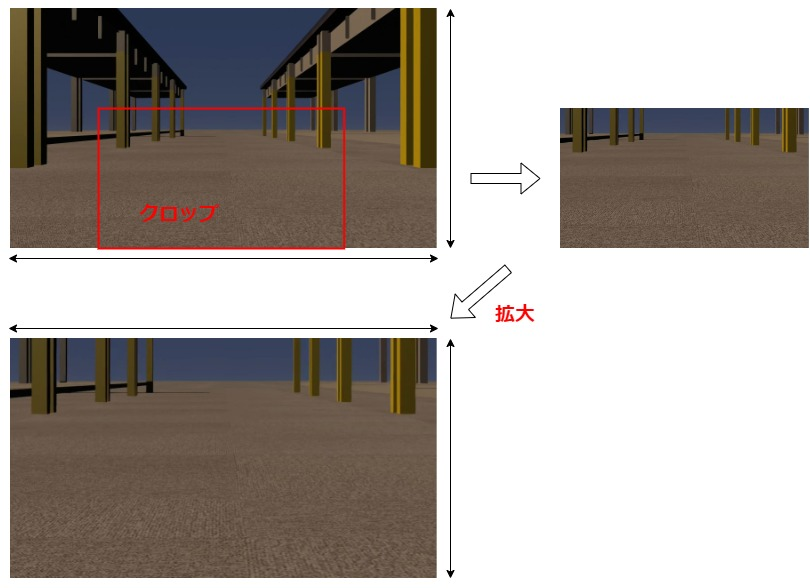
\includegraphics[width=.8\linewidth]{img/8_1.jpg}
  \caption{クロップ手順1}
  \label{taikan:crop1}
  \end{center}
\end{figure}

\begin{figure}[h]
  \begin{center}
  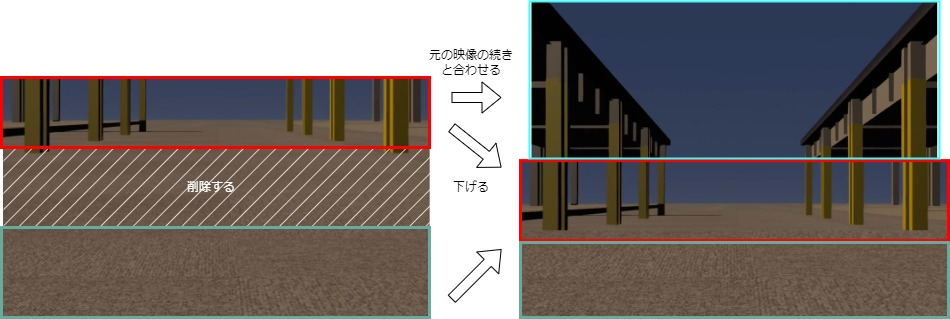
\includegraphics[width=.9\linewidth]{img/8_2.jpg}
  \caption{クロップ手順2}
  \label{taikan:crop2}
  \end{center}
\end{figure}
\clearpage
この実験によって、変化したパラメータについて述べる。クロップ率を増加させることで、映像の縦横の長さが減少し、視野角が減少することが明らかになった。
また、そのほかのパラメータも同時に変化し、クロップ率・視野角が体感速度の変化を制御するパラメータであることを定性的に示した。この時点では定量的な解析はできない。

\subsection{映像クロップによる体感速度の変化の仮説}
クロップ率の変化によって、体感速度が補正される根拠を以下に示す。
\begin{enumerate}
  \item 地上高\\
  手元の景色を排除し、遠くの景色を拡大したため、遠くの景色の流れが遅くなることから、体感速度が遅くなる。
  \item ピクセル\\
  映像のクロップにより、近くに見える映像がより遠い位置になるため、水平面より下の景色の流れが遅くなることで、ピクセルの移動速度が遅くなり、体感速度が遅くなる。
  \item 水平面より下の景色\\
  図\ref{taikan:cropzengo}にクロップ前後の見え方の変化について示す。

  \begin{figure}[h]
    \begin{center}
    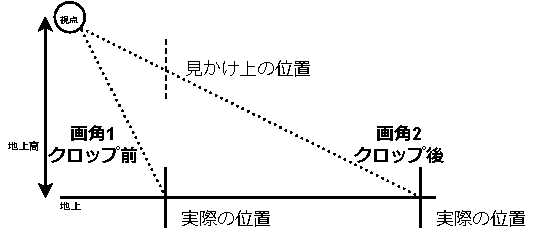
\includegraphics[width=.8\linewidth]{img/9_1.pdf}
    \caption{クロップ前後の見え方の変化}
    \label{taikan:cropzengo}
    \end{center}
  \end{figure}
  映像のクロップにより、クロップ前に見えていたものが前進する。それにより、見かけ上の位置がクロップ前と比べて、近くに見える映像がより遠い位置になるため、水平面よりも下の景色の見え始めが遠くなる。
よって、水平面より下の景色の流れが遅くなることで、体感速度が遅くなる。
\end{enumerate}

本研究以外にも同様の報告として、論文によると、映像のクロップによる体感速度の増強効果が、報告されている。
また、レース用ゲーム等で用いられる手法として取り入れられていることを確認している。

\clearpage

\subsection{体感速度のパラメータの導入}
体感速度変化で最も影響力のあるパラメータが映像のクロップとカメラの画角であることが分かった。
一般的に、走行映像を投影するカメラの画角に加えて、車両のドライバの視野角の変化が体感速度変化に寄与すると考えられている。
また、映像のクロップによってカメラの画角の変化が可能であることが共通の見識として共有されている。
つまり、映像のクロップによって、容易に車両中のドライバの視点の視野角を変化させることができ、体感速度を変化させることができる。
しかし、映像のクロップでは、ドライバの視野角を縮小する場合のみでしか検証ができない。
DSの視野角変更機能を用いることで、カメラの画角・ドライバの視野角を拡大する場合の検証を行うことができる。
そこで、本研究では、画角(視野角)・クロップというパラメータを導入し、映像のクロップを拡張し、
ドライバの視野角の拡大における体感速度の変化に関しても検討を行う。


\section{体感速度モデルの提案}
これまで、スケールスピードと実速度を比較することで、体感速度はスケールスピードと一致せず、単なるスケール比に一致することが明らかになった。
さらに、その過程において体感速度を変化させるパラメータを発見した。列挙した中で最も影響力のあるパラメータが、走行映像のクロップ率やカメラの画角・ドライバの視野角であることが明らかになった。
そこで、走行映像のクロップ率とドライバの視野角を体感速度変化のパラメータとして、体感速度を定式化する手法を提案する。本研究では、実測値との比較として、視野角・ディスプレイ比等、DS環境におけるパラメータを定数とした
幾何学計算による幾何学モデルを提案する。

\subsection{原理}
実車が同じ速度で走行する場合でも、視野角が広い方が、体感速度が速く感じるという現象が生じる基準視野角と、ある視野角での画面上の一方から他方の点にかけてのピクセルの移動距離の比が体感速度の比となる。
図\ref{taikan:pixel}に、ピクセルの移動距離の考え方を示す。
同様の原理として、交通事故で取り上げられるコリジョンコース現象が挙げられる。複数の走行映像において、ピクセルの移動速度が一致する時、体感速度の比と一致していることが望ましい。

\begin{figure}[h]
  \begin{center}
  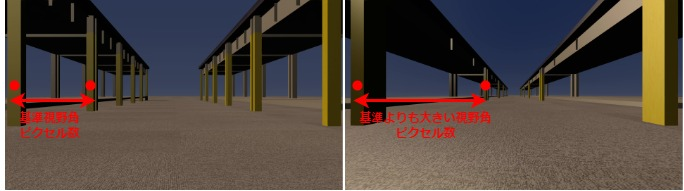
\includegraphics[width=.65\linewidth]{img/11.jpg}
  \caption{ピクセルの移動距離の考え方}
  \label{taikan:pixel}
  \end{center}
\end{figure}

\clearpage
\subsection{体感速度モデルの定式化}
体感速度を求めるために、映像中のポール間の移動の際に映像中の移動ピクセル数と、環境によって決まるパラメータを定式化する。
ここでは、体感速度$v_{sense}$を、視野角の関数$f(h_{fov_v})$で表し、$h_{fov_v}$を、クロップ率の関数$g(n)$で表すことを目標とする。
実際の速度\verb|(実速度とする)|を$v_2$とすると、式\eqref{taikan:eq:model1}、\eqref{taikan:eq:model2}に示す関係式を求める。

\begin{align}
  v_{sense} = f(h_{fov_v})\cdot v_s = f(g(n))\cdot v_s \label{taikan:eq:model1}\\
  h_{fov_v} = g(n) \label{taikan:eq:model2}
\end{align}

まず、ディスプレイのアスペクト比とサイズ(ディスプレイの対角線の長さ)をディスプレイの縦・横の長さに変換する式を式\eqref{taikan:eq:dis1}、\eqref{taikan:eq:dis2}に示す。図\ref{taikan:displaytosize}
にディスプレイ長さの概要と諸条件を示す。

\begin{figure}[h]
  \begin{center}
  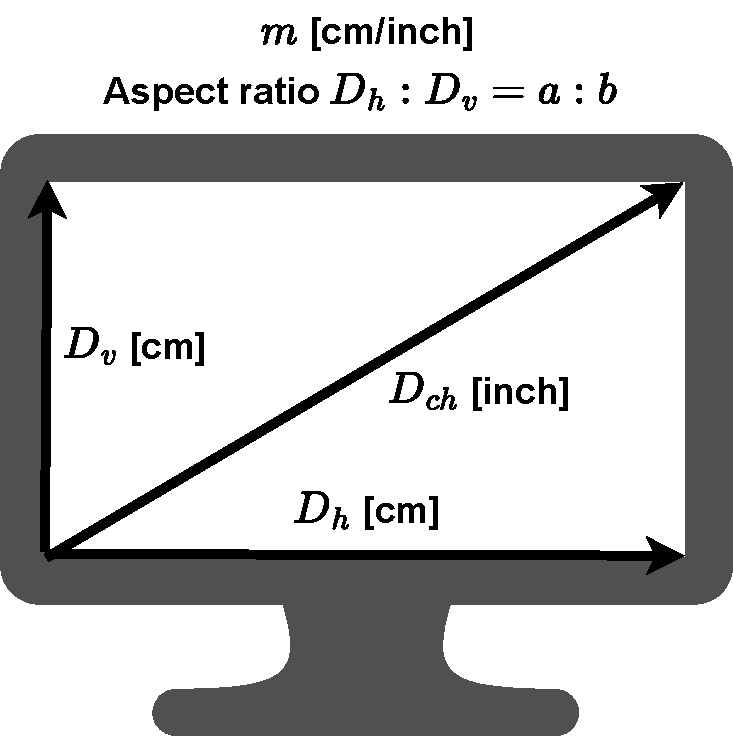
\includegraphics[width=.65\linewidth]{img/12.pdf}
  \caption{ディスプレイ長さの概要と諸条件}
  \label{taikan:displaytosize}
  \end{center}
\end{figure}

\begin{align}
    D_v = D_{ch} \cdot m \cdot \frac{b}{\sqrt{a^2+b^2}} \label{taikan:eq:dis1}\\
    D_h = D_{ch} \cdot m \cdot \frac{a}{\sqrt{a^2+b^2}} \label{taikan:eq:dis2}
\end{align}

$D_v$:ディスプレイの縦の長さ\si{[cm]}、$D_h$:ディスプレイの横の長さ\si{[cm]}、$D_{ch}$:ディスプレイの対角線の長さ\si{[inch]}、
$m$:2.4\si{[cm/inch]}、$a$:ディスプレイの横のアスペクト比:16、$b$:ディスプレイの縦のアスペクト比:9とする。

次に、ディスプレイの縦・横の長さとディスプレイとの視点距離をDS上での水平・垂直方向の基準視野角に式\eqref{taikan:eq:kijun1}、\eqref{taikan:eq:kijun2}を用いて変換する。
図\ref{taikan:kijuntods}に基準視野角とその導出の諸条件を示す。


\begin{figure}[h]
  \begin{center}
  \subfigure[水平方向]{
  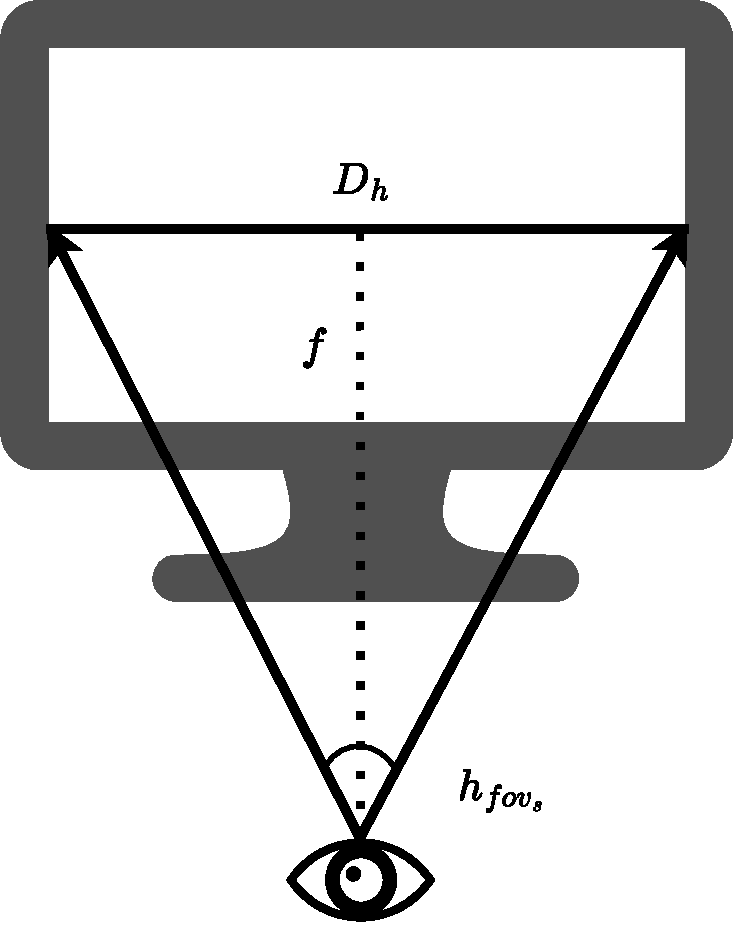
\includegraphics[width=.4\columnwidth]{img/13_1.pdf}
  \label{taikan:kijuntods1}
  }
  \subfigure[垂直方向]{
  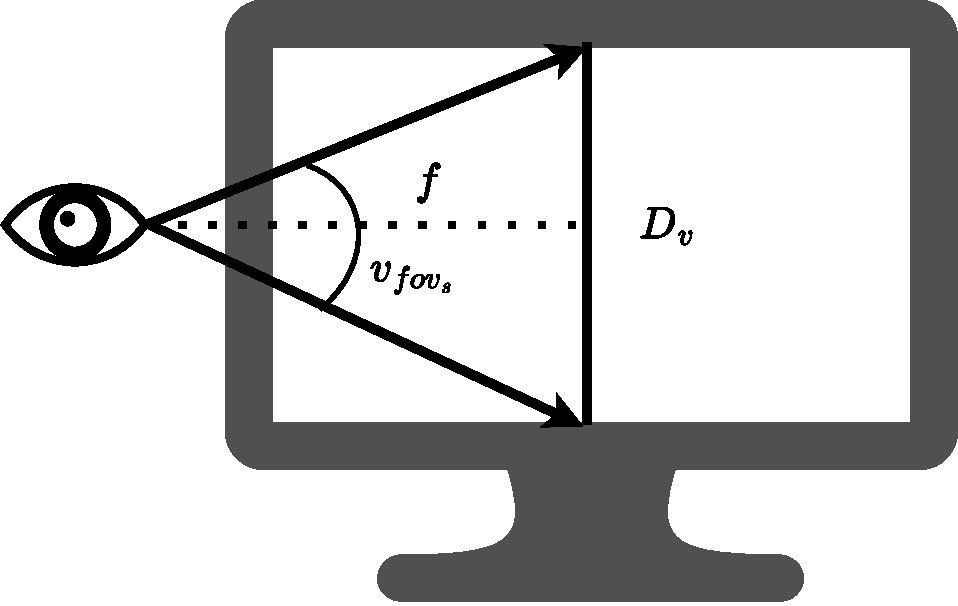
\includegraphics[width=.52\columnwidth]{img/13_2.pdf}
  \label{taikan:kijuntods2}
  }
  \caption{基準視野角とその導出の諸条件}
  \label{taikan:kijuntods}
\end{center}
\end{figure}

\begin{align}
    h_{fov_s} = 2\arctan{\frac{D_h}{2f}} \label{taikan:eq:kijun1}\\
    v_{fov_s} = 2\arctan{\frac{D_v}{2f}} \label{taikan:eq:kijun2}
\end{align}

$h_{fov_s}$:基準水平視野角\si{[degree]}、$v_{fov_s}$:基準垂直視野角\si{[degree]}、$f$:視点距離\si{[cm]}とする。

次に、基準視野角を映像クロップによる視野角に変換する。クロップ率$n$の値域は、$1 \leqq n \leqq 3.5$とする。
$n = 1$の時$h_{fov_s}$、$v_{fov_s}$(基準視野角)とする。
式\eqref{taikan:eq:crop1}、\eqref{taikan:eq:crop2}は、映像のクロップにより、視野範囲が変わることを意味する。
クロップは縦横比を一定とし、映像の中心は変化させない。図\ref{taikan:shiyatocrop}に映像クロップによる視野角とその導出の諸条件を示す。
\clearpage
\begin{figure}[h]
  \begin{center}
  \subfigure[水平方向]{
  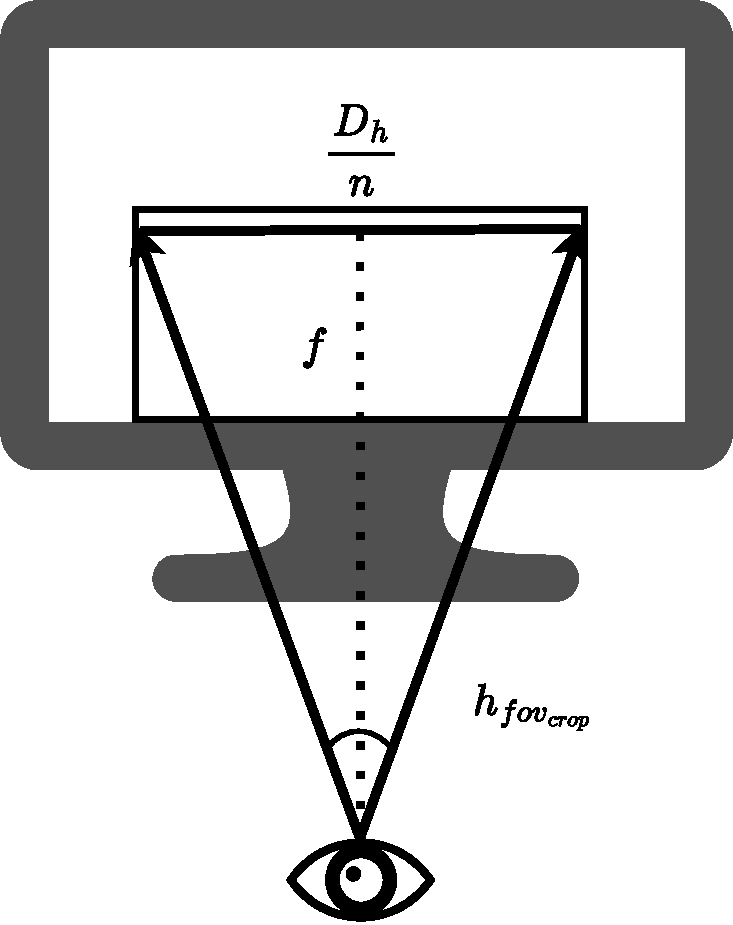
\includegraphics[width=.4\columnwidth]{img/14_1.pdf}
  \label{taikan:shiyatocrop1}
  }
  \subfigure[垂直方向]{
  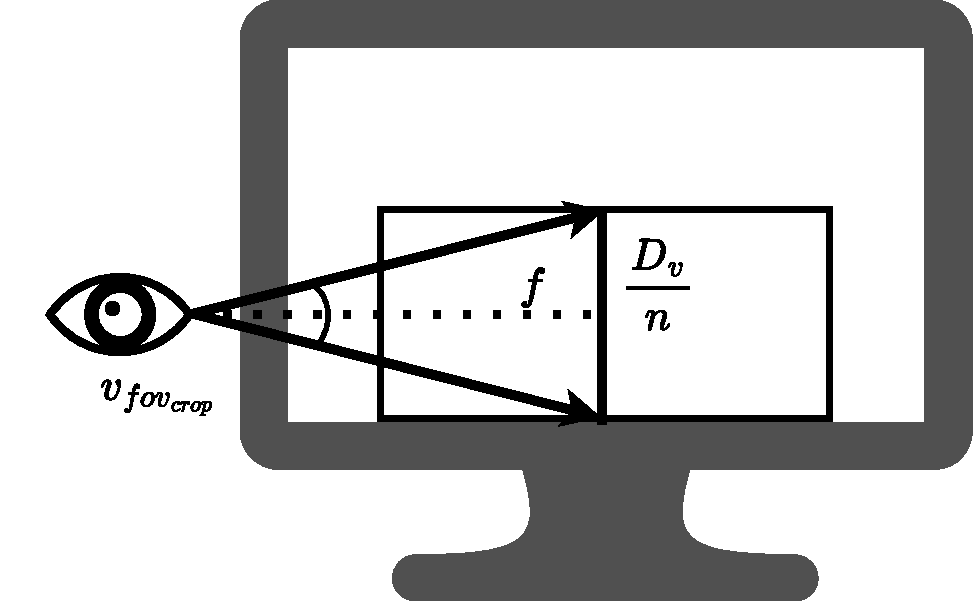
\includegraphics[width=.52\columnwidth]{img/14_2.pdf}
  \label{taikan:shiyatocrop2}
  }
  \caption{映像クロップによる視野角とその導出の諸条件}
  \label{taikan:shiyatocrop}
  \end{center}
\end{figure}

\begin{align}
  h_{fov_{crop}} = 2\arctan{\frac{D_h}{2f\cdot n}} \label{taikan:eq:crop1}\\
  v_{fov_{crop}} = 2\arctan{\frac{D_v}{2f\cdot n}} \label{taikan:eq:crop2}
\end{align}

$h_{fov_{crop}}$:映像クロップによる水平視野角\si{[degree]}、$v_{fov_{crop}}$:映像クロップによる垂直視野角\si{[degree]}、$n$:クロップ率の関数

次に、変数の視野角を基準よりも大きくとる場合に拡張する。つまり、$n<1$を考える。$n = 0.2 \thicksim 1$として拡張し、得られた視野角を変数
$h_{fov_v}$、$v_{fov_v}$とおく、これを体感速度のパラメータとする。$n$は、クロップ率を基準視野角から拡大または縮小するための値として拡張した、視野角拡大率とする。
$n$は、$h_{fov_v}$、$v_{fov_v}$のパラメータである。つまり、体感速度$v_{sense} = f(h_{fov_v}) = f(g(n))$とし、$h_{fov_v}=g(n)$である。
これらの式を、式\eqref{taikan:eq:kakudai1}、\eqref{taikan:eq:kakudai2}に示す。

\begin{align}
  h_{fov_v} = 2\arctan{\frac{D_h}{2f\cdot n}} \label{taikan:eq:kakudai1}\\
  v_{fov_v} = 2\arctan{\frac{D_v}{2f\cdot n}} \label{taikan:eq:kakudai2}
\end{align}

$h_{fov_v}$:水平視野角変数\si{[degree]}、$v_{fov_v}$:垂直視野角変数\si{[degree]}、$n$:視野角拡大率とする。

次に、体感速度は、基準視野角と水平視野角変数におけるそれぞれの映像のポール間ピクセル数の比を、実速度に乗ずることで式\eqref{taikan:eq:vsense}により求められる。

\begin{align}
  v_{sense} = \frac{px_v}{px_s}v_s = m_{sense}\cdot v_s \label{taikan:eq:vsense}
\end{align}

$px_v$:$h_{fov_v}$におけるポール間ピクセル数\si{[px]} (実測値)、$px_s$:$h_{fov_s}$におけるポール間ピクセル数\si{[px]}実測値、$v_{sense}$:体感速度\si{[km/h]}、$v_s$:実速度\si{[km/h]}、$m_{sense}$:ポール間ピクセル数の比とする。

図\ref{taikan:px}に視野角の違いによるポール間ピクセル数の違いを示す。

\begin{figure}[h]
  \begin{center}
  \subfigure[基準視野角]{
  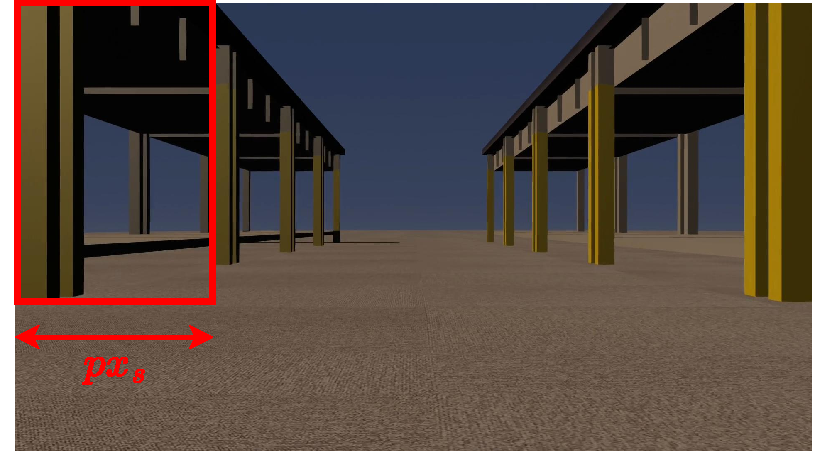
\includegraphics[width=.8\columnwidth]{img/15_1.pdf}
  \label{taikan:pxs}
  }
  \subfigure[変化視野角(増加)]{
  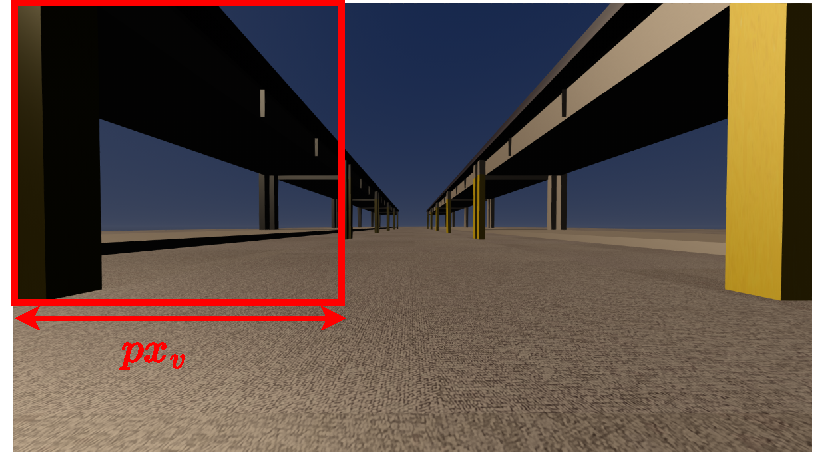
\includegraphics[width=.8\columnwidth]{img/15_2.pdf}
  \label{taikan:pxv}
  }
  \caption{視野角の違いによるポール間ピクセル数の違い}
  \label{taikan:px}
  \end{center}
\end{figure}

次に、$v_{sense}=f(h_{fov_v})$となる$f$を導きたい。$v_s$は一定として考えているため、$m_{sense}=f(h_{fov_v})$を導く。ここで、
視野角変数$h_{fov_v}$において、映像中のボールが画面の端にあるとする。(視点とディスプレイの短辺は$h_{fov_v}$の角度をなす。)
そこから、次のボールが画面の端になるように縦横比一定でクロップした時のクロップ率を視野辺ピクセル倍率$n_{p_{\to}p}$とする。
基準視野角においても同様に、$n_{p_{\to}p_s}$(基準視野角の場合の$n_{p_{\to}p_s}$)を求める。なお、遠近法より、$n_{p_{\to}p_s} = 2$であることが一般的に知られている。すると、
$m_{sense}$は、図\ref{taikan:kika}に示す視野角に関する幾何学を用いて、
式\eqref{taikan:eq:kika1}\verb|~|\eqref{taikan:eq:kika3}のように求めることができる。

\begin{figure}[h]
  \begin{center}
  \subfigure[基準視野角の幾何学]{
  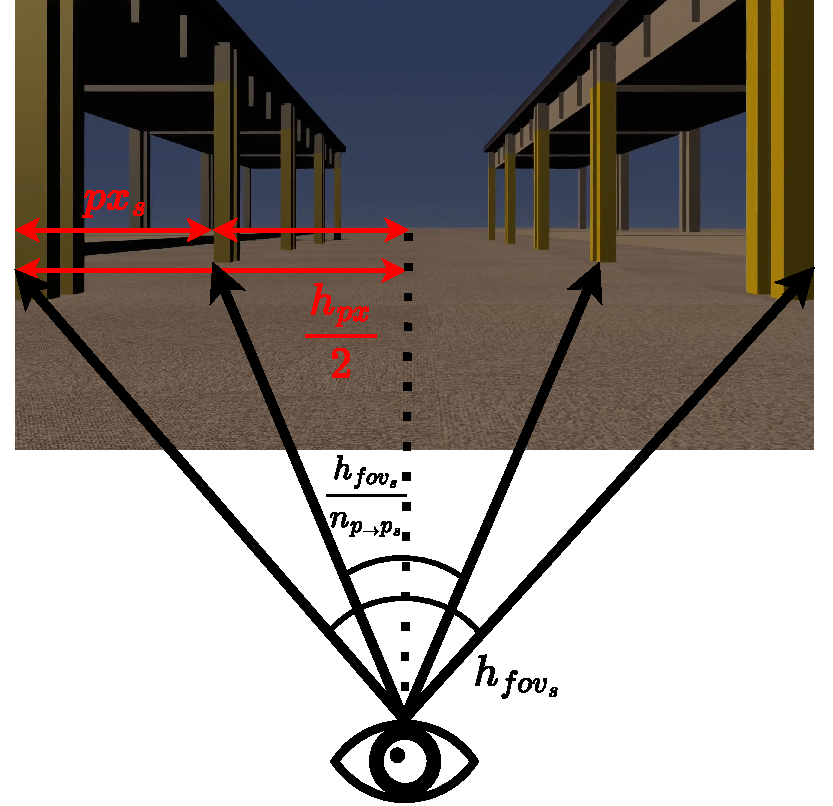
\includegraphics[width=.45\columnwidth]{img/16_2.pdf}
  \label{taikan:kika1}
  }
  \subfigure[変化視野角の幾何学]{
  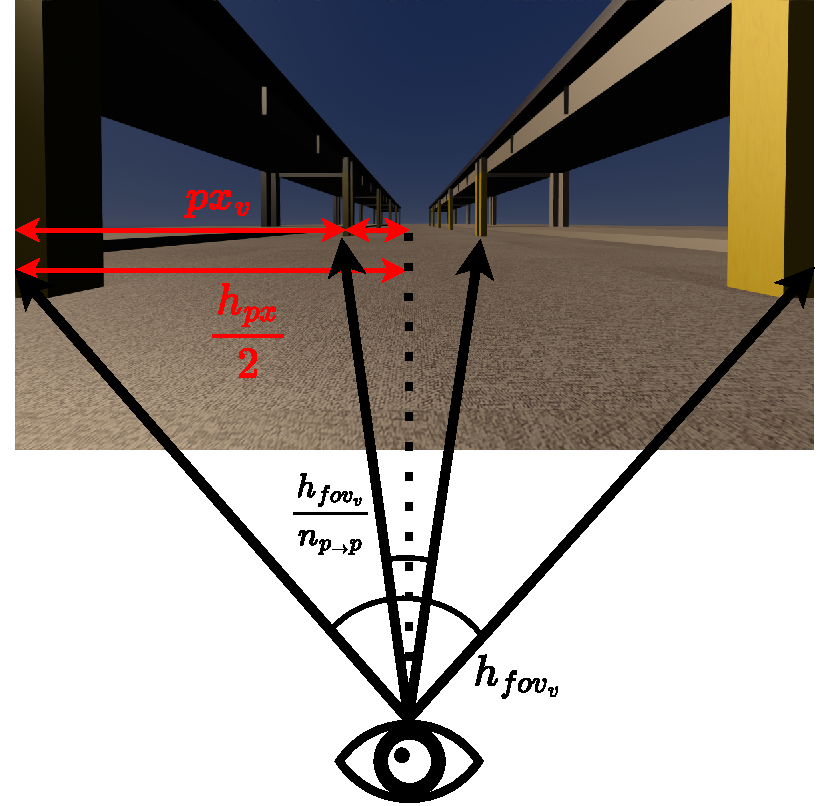
\includegraphics[width=.45\columnwidth]{img/16_3.pdf}
  \label{taikan:kika2}
  }
  \subfigure[$n_{p_{\to}p}$について]{
  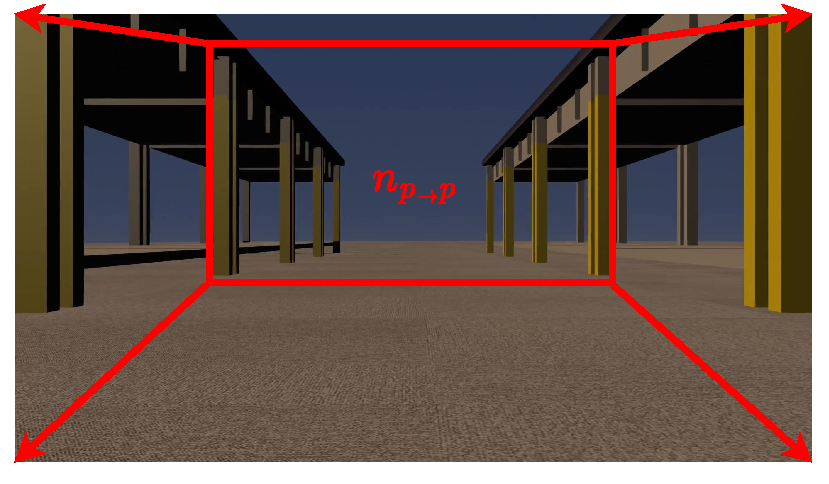
\includegraphics[width=.45\columnwidth]{img/16_1.pdf}
  \label{taikan:kika3}
  }
  \caption{視野角に関する幾何学}
  \label{taikan:kika}
  \end{center}
\end{figure}

\begin{align}
  px_s &= \frac{h_{px}}{2} - \frac{h_{px}}{2}\Bigg(\frac{\tan\frac{h_{fov_s}}{2\cdot n_{p_{\to}p_s}}}{\tan{\frac{h_{fov_s}}{2}}}\Bigg) = \frac{h_{px}}{2}\Biggl(1-\frac{\tan{\frac{h_{fov_s}}{4}}}{\tan{\frac{h_{fov_s}}{2}}}\Biggr) \label{taikan:eq:kika1}\\
  px_v &= \frac{h_{px}}{2} - \frac{h_{px}}{2}\Bigg(\frac{\tan\frac{h_{fov_v}}{2\cdot n_{p_{\to}p_v}}}{\tan{\frac{h_{fov_v}}{2}}}\Bigg) = \frac{h_{px}}{2}\Biggl(1-\frac{\tan{\frac{h_{fov_v}}{2\cdot n_{p_{\to}p}}}}{\tan{\frac{h_{fov_v}}{2}}}\Biggr) \label{taikan:eq:kika2}\\
  m_{sense} &= \frac{px_v}{px_s} = \frac{\Biggl\{\frac{h_{px}}{2}\Bigg(1-\frac{\tan\frac{h_{fov_v}}{2\cdot n_{p_{\to}p}}}{\tan\frac{h_{fov_v}}{2}}\Bigg)\Biggr\}}{\Biggl\{\frac{h_{px}}{2}\Bigg(1-\frac{\tan\frac{h_{fov_s}}{4}}{\tan\frac{h_{fov_s}}{2}}\Bigg)\Biggr\}} = \frac{1-\frac{\tan\frac{h_{fov_v}}{2\cdot n_{p_{\to}p}}}{\tan\frac{h_{fov_s}}{2}}}{1-\frac{\tan\frac{h_{fov_s}}{4}}{\tan\frac{h_{fov_s}}{2}}} = f(h_{fov_v}) \label{taikan:eq:kika3}
\end{align}

$h_{px}$:ディスプレイの横のピクセル比\si{[px]}(1920 \si{[px]})、$n_{p_{\to}p}$:$h_{fov_v}$における視野辺ピクセル倍率(実測値)、
$n_{p_{\to}p_s}$:$h_{fov_s}$における視野辺ピクセル倍率(定数値:2)。

ここで、幾何学的に求められた$f(m_{sense})$を、体感速度$v_{sense}$の理論式とする。$h_{fov_v}$を$v_{sense}$に変換する。式\eqref{taikan:eq:kika3}を整理すると、
式\eqref{taikan:eq:final}のようになる。

\begin{equation}
  \begin{split}
    m_{sense} &= \frac{px_v}{px_s} = \frac{1-\frac{\tan\frac{h_{fov_v}}{2\cdot n_{p_{\to}p}}}{\tan\frac{h_{fov_v}}{2}}}{1-\frac{\tan\frac{h_{fov_s}}{2\cdot n_{p_{\to}p_s}}}{\tan\frac{h_{fov_s}}{2}}} = \frac{1-\frac{\tan\frac{h_{fov_v}}{2\cdot n_{p_{\to}p}}}{\tan\frac{h_{fov_v}}{2}}}{1-\frac{\tan\frac{28}{2\cdot 1.986}}{\tan\frac{28}{2}}}=1.923\cdot \Bigg(1 - \frac{\tan\frac{h_{fov_v}}{2\cdot n_{p_{\to}p}}}{\tan\frac{h_{fov_v}}{2}}\Bigg)\\ \label{taikan:eq:final}
    &= f(h_{fov_v}, n_{p_{\to}p}) = 1.923\cdot \Bigg(1 - \frac{\tan\frac{h_{fov_v}}{2\cdot 1.078415307\cdot e^{0.011995591\cdot h_{fov_v}}}}{\tan\frac{h_{fov_v}}{2}}\Bigg) = f(h_{fov_v})
  \end{split}
\end{equation}

よって、式\eqref{taikan:eq:final}は、式\eqref{taikan:eq:sensefinal}のようになる。

\begin{align}
  v_{sense} = 19.30\Bigg(1-\frac{\tan\frac{h_{fov_v}}{2\cdot 1.078415307\cdot e^{0.011995591\cdot h_{fov_v}}}}{\tan\frac{h_{fov_v}}{2}}\Bigg) \label{taikan:eq:sensefinal}
\end{align}

$n_{p_{\to}p}$は、式\eqref{taikan:eq:kaiki}による回帰曲線とした。

\begin{align}
  n_{p_{\to}p} = 1.078415307\cdot e^{0.011995591\cdot h_{fov_v}} \label{taikan:eq:kaiki}
\end{align}

この式を基準視野角における倍率をクロップ倍率を$m$として、正規化すると、式\eqref{taikan:eq:mseiki}

\begin{align}
  m_{sense} = \frac{px_v}{px_s} = \frac{1-\frac{\tan\frac{h_{fov_v}}{2\cdot p_{p_{\to}p}}}{\tan\frac{h_{fov_v}}{2}}}{1-\frac{\tan\frac{h_{fov_s}}{2\cdot n_{p_{\to}p_s}}}{\tan\frac{h_{fov_s}}{2}}} = \frac{1-\frac{\tan\frac{h_{fov_v}}{2\cdot n_{p_{\to}p}}}{\tan\frac{h_{fov_s}}{2}}}{1-\frac{\tan\frac{h_{fov_s}}{2\cdot 1.986}}{\tan\frac{h_{fov_s}}{2}}} = \frac{1-\frac{\tan\frac{h_{fov_v}}{2\cdot n_{p_{\to}p}}}{\tan\frac{h_{fov_v}}{2}}}{1-\frac{\tan\frac{h_{fov_s}}{2\cdot 1.986\cdot m}}{\tan\frac{h_{fov_s}}{2}}} \label{taikan:eq:mseiki}
\end{align}
$$m=1/1.986$$

よって、以上をまとめると、式\eqref{taikan:eq:v}、\eqref{taikan:eq:fov}となる。

\begin{align}
  v_{sense} &= 19.30\cdot\Bigg(1-\frac{\tan\frac{h_{fov_v}}{2\cdot n_{p_{\to}p}}}{\tan\frac{h_{fov_v}}{2}}\Bigg) = f(h_{fov_v})\cdot v_s = f(g(n))\cdot v_s \label{taikan:eq:v}
\end{align}
\begin{align}
  h_{fov_v} &= 2\arctan\frac{D_h}{2f\cdot n} \label{taikan:eq:fov}
\end{align}

以上により、視野角、クロップ率を体感速度の倍率に変換する以下の式を導いた。
\begin{align*}
  v_{sense} = f(h_{fov_v})\cdot v_s = f(g(n))\cdot v_s
\end{align*}
\begin{align*}
  h_{fov_v} = g(n)
\end{align*}

この定式モデルを用いることで、基準視野角に対して、任意の視野角における体感速度を求めることができる。
また、視野角はクロップ率の関数であるため、任意のクロップ率に対しての体感速度を求めることもできる。
この定式もでるでは、パラメータを視野角としたが、その他にも、体感速度を決める環境のパラメータとして、ディスプレイ長さや、
インチ数等も用いることができる。したがって、走行映像の取得環境に応じた変数と固定値を入れ替えることで、あらゆる環境の幾何学的なパラメータに対応した定式もでると言える。
このモデルの大まかな特性を求めるために、$m_{sense}$を累乗で近似すると、式\eqref{taikan:eq:shijo}となり、
体感速度は、式\eqref{taikan:eq:shijov}で表すことができる。

\begin{align}
  m_{sense} = 0.086537715\cdot h_{fov_v}^{0.615630604} \label{taikan:eq:shijo}\\
  v_{sense} = 0.86537715\cdot h_{fov_v}^{0.615630604} \label{taikan:eq:shijov}
\end{align}

従って、$v_{sense}$は、視野角の$n$乗根に比例する軌跡となる。その概形は、緩やかに上昇する軌跡である。

\section{提案モデルの検証実験}
これまで、体感速度の定式化を提案した。ここでは、提案したモデルが正しいことを実証するための検証実験に関して述べる。
前述の体感速度のモデルを実証するために、以下の手順で実験を行った。

\subsection{定式化モデルと実測値の比較}
前と同様のRCカーの走行環境を模したDS走行環境において走行実験を行う。基準視野角における速度と映像のクロップ率を変化させた時の体感速度との比率をポール間ピクセル数の計測により求める。
ポール間をディスプレイの横幅まで拡大し、ディスプレイの解像度をその拡大倍率で割ることでポール間ピクセル数が導出される。
今回、定式化したモデルは、水平視野角をパラメータとして用いているが、
DS環境設定では、垂直視野角を設定値とする仕様であるため、水平視野角を垂直視野角に変換した値をDS環境の視野角設定に用いる。
基準視野角(垂直視野)を20度として、DS環境設定の視野角変更機能により、視野角を変化させる。
図\ref{taikan:shiyaset}にDSの視野角設定を示す。

\begin{figure}[h]
  \begin{center}
  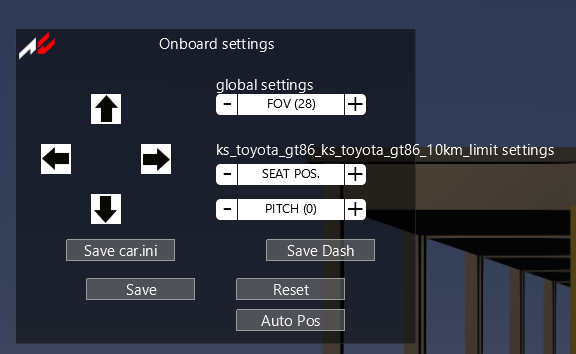
\includegraphics[width=.65\linewidth]{img/17.png}
  \caption{DSの視野角設定}
  \label{taikan:shiyaset}
  \end{center}
\end{figure}

DS乗で定速走行した映像を解析し、基準視野角とポール間ピクセル数を実測する。基準視野角と、ある視野角の関係から幾何学的にポール間ピクセル数を計算し、定速度値に乗じることで体感速度を実測する。
幾何学的な倍率は一部実測値を含む。その後、実測値と幾何学モデルとの一部実測値を含む。実測値と幾何学モデルとの一致を確認する。基準視野角で実速度10 \si{[km/h]}、体感速度10 \si{[km/h]}の映像と、
ある視野角を変えて実速度10 \si{[km/h]}、体感速度17 \si{[km/h]}(単位時間のポール間の移動ピクセル数が1.7倍になったもの)の映像と、基準視野角で実測度17 \si{[km/h]}、体感速度17 \si{[km/h]}、体感速度17 \si{[km/h]}
(単位時間に通過する柱の数が1.7倍になったもの)の映像を比較して、この仮説を検証する。

\begin{figure}[h]
  \begin{center}
  \subfigure[基準視野角]{
  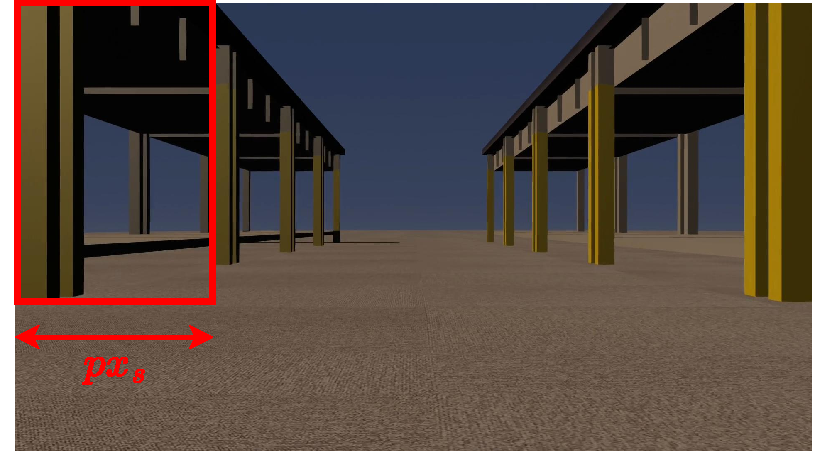
\includegraphics[width=.45\columnwidth]{img/17_1.pdf}
  \label{taikan:pxs_1}
  }
  \subfigure[変化視野角(増加)]{
  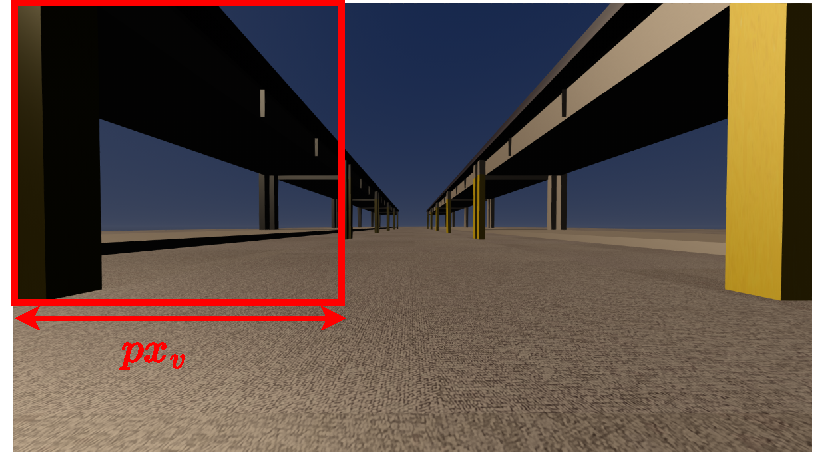
\includegraphics[width=.45\columnwidth]{img/17_2.pdf}
  \label{taikan:pxv_1}
  }
  \subfigure[変化視野角(増加)]{
  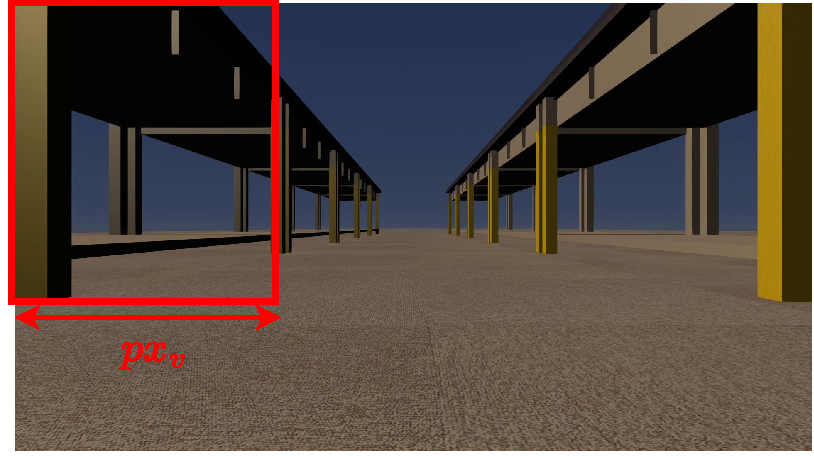
\includegraphics[width=.45\columnwidth]{img/17_3.pdf}
  \label{taikan:pxv_2}
  }
  \caption{視野角の違いによるポール間ピクセル数の違い}
  \label{taikan:px_sv}
  \end{center}
\end{figure}

一例として、基準視野角に対する視野角での見え方を図\ref{taikan:px_sv}に示す。赤線の横辺のピクセル数を求める。

\subsection{実験条件}
今回の実験で用いた環境と実験条件を示す。本研究で定式化したモデルは、水平視野角をパラメータとして用いているが、DS環境設定では、垂直視野角を設定値とする仕様であるため、水平視野角を垂直視野角に変換した値をDS環境の視野角設定に用いる。
その指定値を$v_{fov}$と、cropとして、表\ref{taikan:table2}に示す。本研究では、クロップ率をパラメータとして定めると、$v_{fov_v}$を求めることができるため、クロップ率cropに対応する視野角を用いる。

\begin{table}[h]
  \centering
  \caption{水平視野角の指定値$v_{fov}$とクロップ率cropとの対応}
  \scalebox{.6}{
  \begin{tabular}[t]{rrrrrrrrrrrrrrrrrrrrrrrrr}
  \toprule
  $v_{fov}$\si{[degree]}:&8&9&10&11&12&13&14&15&16&17&19&20&21&23&25&28&30&34&39&44&52&63&78&102\\
  \midrule
  crop:&0.2&0.3&0.4&0.5&0.6&0.7&0.8&0.9&1.0&1.1&1.2&1.3&1.4&1.5&1.6&1.7&1.8&2&2.2&2.4&2.6&2.8&3.1&3.5\\
  \bottomrule
  \label{taikan:table2}
  \end{tabular}}
\end{table}%

また、本実験で使用した環境について表\ref{taikan:table3}に示す。

\begin{table}[h]
  \centering
  \caption{本研究で使用した環境}
  \scalebox{.8}{
  \begin{tabular}[t]{c}
    \toprule
    環境\\
    DS:Asetto Corsa 1.16\\
    ディスプレイ:iiyama ProLite P2474HS 23.6インチ full HD 1920x1080 60 Hz\\
    MOD:ACContentManager 0.8.2569.39678\\
    カメラ:gopro hero8\\
    CGソフト:Blender\\
    \bottomrule
    \label{taikan:table3}
  \end{tabular}}
\end{table}

\subsection{定式化モデルの検証方法}
DS走行環境においてピクセル倍率を実測する。まず、動画編集ソフトを用いて、映像中のポール間距離を画面上の左右のサイズになるように拡大し、
左右のサイズを拡大率で割ることで、走行映像におけるポール間ピクセル数$n_{p_{\to}p}$を求める。これを基準視野角と視野角を変化させた時で測定し、
基準視野角に対する、ある視野角でのピクセル数の比を求めて、体感速度比とする。次に、体感速度比と実際の速度を掛けて体感速度を導出する。
以上の手順で体感速度を求めて、視野角との特性をグラフ上にプロットする。定式モデルに、実験条件で示した視野角と先に求めた拡大率を代入し、体感速度を導出する。
定式モデルの視野角と体感速度の特性をグラフ上にプロットする。定式モデルでの拡大率は、視野角の変数で表すことが困難であるため、実測値を用いる。

\subsection{体感速度を変化させる効果の検証}
定式化モデルが体感速度を変化させる効果を与えることの検証として、以下の手順を行う。
\begin{enumerate}
  \item 基準視野角(垂直28度)、実速度が基準速度と等しく10 \si{[km/h]}、体感速度が基準速度と等しい映像を取得する。
  \item ある視野角(垂直102度)、実速度10 \si{[km/h]}、体感速度17 \si{[km/h]}での走行映像を取得する。
  \item 基準視野角(垂直28度)、実速度17 \si{[km/h]}、体感速度17 \si{[km/h]}での走行映像を取得する。
  \item 基準視野角・実速度17 \si{[km/h]}、体感速度17 \si{[km/h]}の映像と、ある視野角(垂直102度)、実速度17 \si{[km/h]}、体感速度17 \si{[km/h]}(単位時間のポールの移動ピクセル数が1の時の1.7倍になったもの)の映像を取得する。
\end{enumerate}

\subsection{実験結果}

\subsubsection{定式化モデルと実測値の比較}
実験結果を図\ref{taikan:kekka1}、\ref{taikan:kekka2}に示す。

\begin{figure}[h]
  \begin{center}
  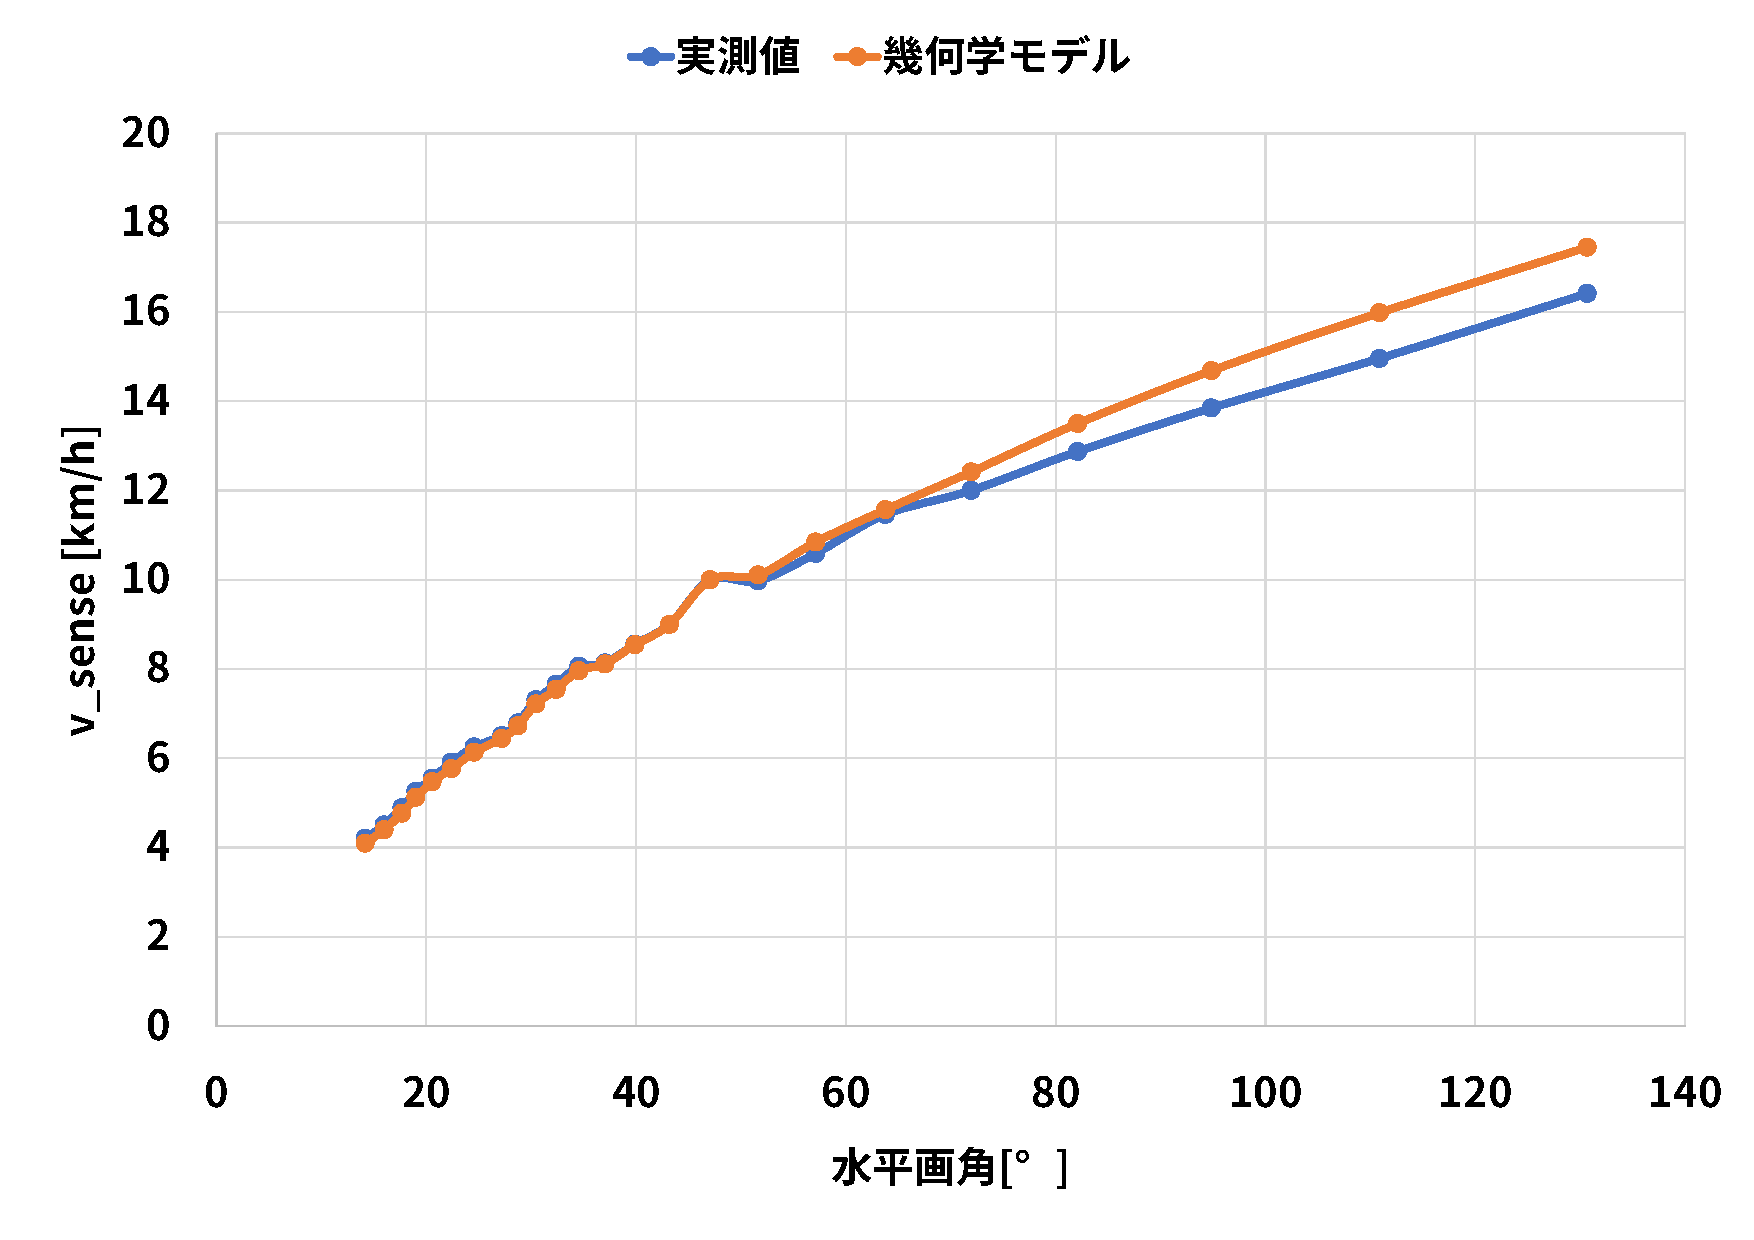
\includegraphics[width=.85\linewidth]{img/19.pdf}
  \caption{水平視野角と体感速度の特性}
  \label{taikan:kekka1}
  \end{center}
\end{figure}

幾何学モデルの理論式を式\eqref{taikan:eq:kekka1}\verb|~|\eqref{taikan:eq:kekka4}に示す。$n_{p_{\to}p}$は、実測である。

\begin{align}
  v_{sense} = 19.30\Bigg(1-\frac{\tan\frac{h_{fov_v}}{2\cdot n_{p_{\to}p}}}{\tan\frac{h_{fov_v}}{2}}\Bigg) \label{taikan:eq:kekka1}
\end{align}
\begin{align}
  h_{fov_v} = 2\arctan\Bigg(\frac{D_h}{2f\cdot n}\Bigg) \label{taikan:eq:kekka2}
\end{align}
\begin{align}
  n = \frac{D_h}{2f\tan\frac{h_{fov_v}}{2}} \label{taikan:eq:kekka3}
\end{align}
\begin{align}
  v_{fov_v} = 2\arctan\frac{D_v}{2f\cdot n} \label{taikan:eq:kekka4}
\end{align}

以上の式\eqref{taikan:eq:kekka5}、\eqref{taikan:eq:kekka6}を用いて、$v_{fov_v}$を、$h_{fov_v}$に変換し、$h_{fov_v}$を変数とする。

\begin{align}
  h_{fov_v} = 2\arctan\frac{D_h}{2f\cdot n} \label{taikan:eq:kekka5}
\end{align}
\begin{align}
  v_{sense} = 19.30\cdot \Bigg(1-\frac{\tan\frac{h_{fov_v}}{2\cdot n_{p_{\to}p}}}{\tan{\frac{h_{fov_v}}{2}}}\Bigg) \label{taikan:eq:kekka6}
\end{align}

\begin{figure}[h]
  \begin{center}
  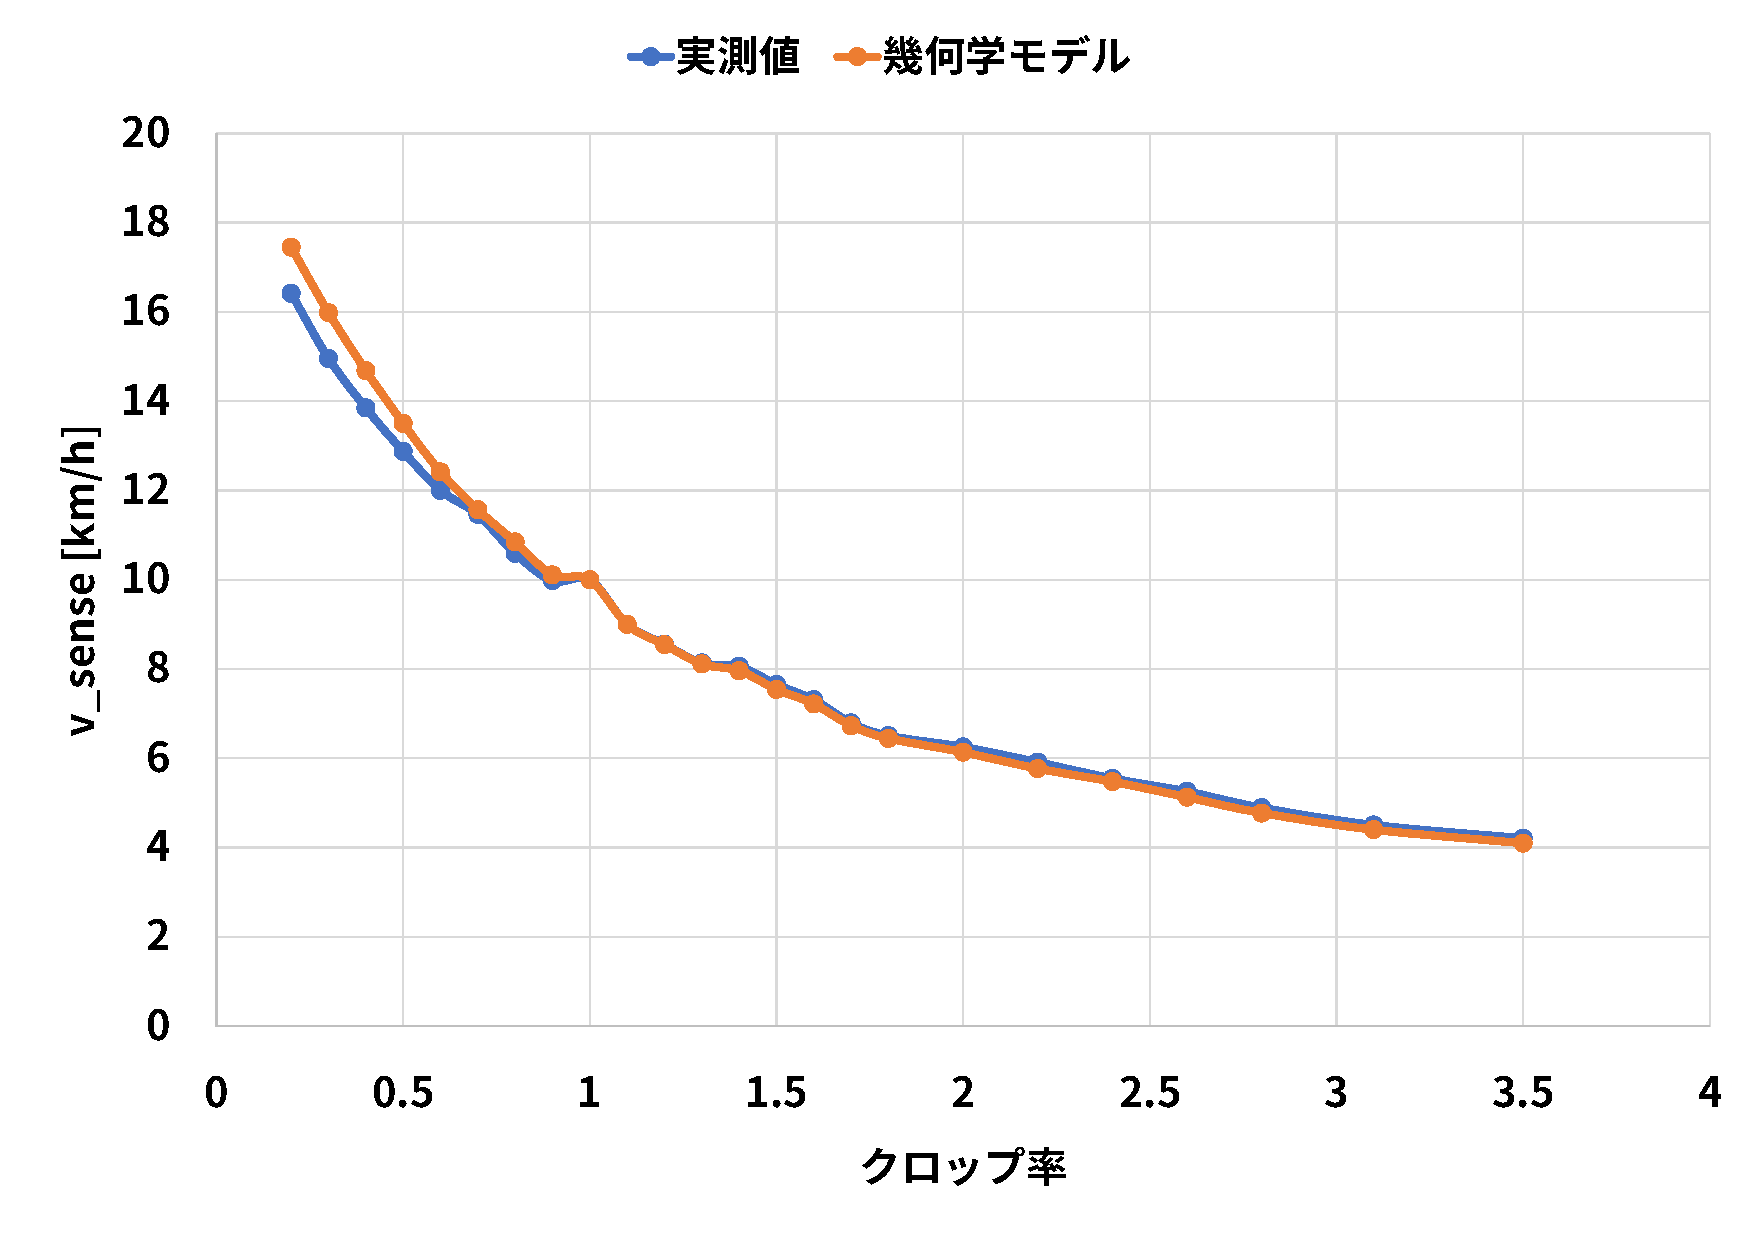
\includegraphics[width=.85\linewidth]{img/20.pdf}
  \caption{クロップ率と体感速度の特性}
  \label{taikan:kekka2}
  \end{center}
\end{figure}

\clearpage

\subsubsection{体感速度を変化させる効果の検証}
実験結果を以下に示す。
\begin{enumerate}
  \item ピクセル比と実速度比の一致の確認\\
  基準視野角(垂直28度)、実速度が基準速度と等しく10 \si{[km/h]}、体感速度が基準速度と等しい映像に関して\\
  ポール間移動時間:5.25秒、ポール間ピクセル数:480 \si{[px]}\\
  ある視野角(垂直120度)、実速度10 \si{[km/h]}、体感速度17 \si{[km/h]}での走行映像に関して\\
  ポール間移動時間:5.25秒、ポール間ピクセル数:788 \si{[px]}\\
  時間比:$5.5\div 3.05 = 1.7213$\\
  ピクセル比:$788\div 480 = 1.64$\\
  体感速度:時間比$\times 10 = 17.213 = 17$ \si{[km/h]}\\
  誤差:$\frac{17.2-16.4}{16.4}\times 100 = 4.878 = 4.9$ \%
  \item 体感速度比(時間比)とピクセル比の一致の確認\\
  ある視野角(垂直102度)、実速度10 \si{[km/h]}、体感速度17 \si{[km/h]}での走行映像に関して、\\
  ポール間移動距離:5.25秒、ポール間ピクセル数:788 \si{[px]}\\
  基準視野角(垂直28度)、実速度17 \si{[km/h]}、体感速度17 \si{[km/h]}での走行映像に関して\\
  ポール間移動距離:2.96秒、ポール間ピクセル数:463 \si{[px]}\\
  時間比:$5.25\div 2.96 = 1.7736$\\
  ピクセル比:$788\div 463 = 1.7019$\\
  体感速度:$1.7736\times 10 = 17.7$ \si{[km/h]}\\
  誤差:$(1.7736-1.7019)\div 1.7019 \times 100 = 4.2129 = 4.2$\%
\end{enumerate}
よって、これらの定式化が実測と同程度であることを確認した。

\section{考察}
\subsection{定式化モデルと実測値の比較に関して}
視野角-体感速度特性において、視野角の増加に伴って体感速度は緩やかに増加する。
この結果は定説と一致している。特性の概形は、おおよそ視野角の$n$乗根に比例すると考えられる点が仮定と一致していた。
基準視野角よりも小さな視野角値である時は、比例的に増加するが、基準視野角以上の値をとると、理論値、実測値ともに体感速度の変化率は緩やかになる。
また、視野角が70度以上の値をとると、理論値と、理論値との差が大きくなる。視野角が基準視野角よりも大きな値である映像は、基準視野角よりも小さな視野角の映像と比べて、映像の奥行きが大きくなり、映像自体が歪んでいることが分かる。
このことから、定式化モデルとして、ひずみに関するパラメータを考慮する必要があることが分かる。
なお、今回の定式化モデルでは、理想的な2次元の映像として考えていたため、このひずみに関しては考慮していない。考慮するためには、3次元の立体映像に関する知見が必要である。
クロップ率-体感速度特性について、クロップ率の増加に伴い体感速度は急激に減少する。
クロップ率を増加させると視野角が減少するため、視野角の減少により体感速度が減少することが定説通りであることを確認した。
クロップ率が1よりも大きな値をとる場合は、視野角を増加させていることと考えると、先に述べた点と一致している。

\subsection{体感速度を変化させる効果の検証}
ピクセル比と実速度比の一致の確認に関して、時間比と速度比は、定義通り一致していたが、単位時間当たりの移動ピクセル数と実速度比に関しては、4.9 \% 程の誤差がみられた。
DSでは小数点以下の速度は表示されないため、この誤差は、DS上における実速度の誤差であると考えられる。
このことから、体感速度に関する仮説として、視野角の変化によって、走行映像中のポール間ピクセル数が変化していることが体感速度の変化を表していることが実証された。
体感速度比とピクセル比の一致に関して、視野角をパラメータとして求めた体感速度と、その体感速度値と一致する実速度の映像では、単位時間当たりに進行するピクセルの比率がほとんど一致するため、単位時間当たりに移動するポール数は一致しないが、単位時間当たりに進行するピクセル数が一致することが確認された。
この結果より、体感速度を支配するパラメータとして提案されていた、映像中の風景線が流れるスピードが一致していることが分かる。
また検証により、視野角やクロップ率をパラメータとして、幾何学的に単位時間当たりに移動するピクセル比を導出する手法を用いた体感速度のモデルが正しいことが明らかになった。

\section{おわりに}
本章では、走行映像における体感速度を支配するパラメータを明らかにし、そのパラメータを用いて、体感速度の変化率のモデルを定量化した。
映像のクロップ率と映像の視野角(撮影画角) が最も影響力の大きいパラメータであることが明らかになった。
体感速度のモデルとして、映像の視聴環境とクロップ率と視野角を用いて幾何学的な計算によって導出したモデル(幾何学モデル)を提案した。
幾何学モデルが正しいことを検証するために、移動ピクセル数の実測値との比較により、検証実験により、実速度が異なる映像でも、体感速度が一致する視野角を設定することで、
単位時間当たりの移動ピクセル数が一致し、映像中の風景線が流れるスピードが一致したことから、幾何学モデルが正しいことを明らかにした。
提案した幾何学モデルに一部実測値を用いている点や、視野角を大きくしたときに生じた立体的なひずみが生じることが明らかになり、立体視野角を考慮した幾何学が必要であることに関して、
新たな知見を得た。この知見を基にモデルの改良に関する検討の余地があり、今後の課題とする。
本研究は、人間の視野が走行映像全体に均一に焦点しているという仮定の上で行っていた。今後は、人間の集中点・集中視野によって変化する体感速度のモデルに関して研究を行う予定である。

\chapter{LiDARのみのSLAMで作成された環境地図の評価}
\section{はじめに}
SLAMは、GPS、GNSS等による絶対的な位置座標を得ることができない環境での自律移動ロボットへの導入ができる点で注目されている。
LiDARのSLAMを行う場合は、LiDARによる位置計測(スキャン)と、ロータリーエンコーダ等の内界センサによる移動履歴(デッドレコニング、オドメトリ)を組み合わせることが一般的かつ、内界センサによるオドメトリとの併用が前提とされたアルゴリズムが主流である。

実用の現状において、つくばチャレンジ等をはじめとする屋外自律移動ロボットコンテストでは、GNSSを組み合わせている場合が多い。
LiDARのSLAMにおける内界センサやGNSS等との併用のメリットは、位置情報の補正が優位であるからである。
しかし、オドメトリの有無に関して、ロータリーエンコーダを用いる場合は、タイヤのスリップ等による誤差の蓄積による地図の精度の誤差をもたらし、精度の良いIMU、GNSS等の内界センサを用いる場合は、導入コストがかかるといったデメリットが考えられる。
LiDAR導入のメリットは、カメラを用いる場合での欠点であった、測定精度や暗闇であっても精度に影響がなく、夜間や雨天時に利用できることである。
SLAMにおける、LiDARのハードウェア的な要求スペックに関しては、2次元の地図作成のみの機能に限定するならば、ほとんど限定されない。
むしろ、LiDARを用いたSLAMアルゴリズムの性能に依存する。

LiDARを用いたSLAMのアルゴリズムに関しては、いくつかの種類がある。
LiDARによって計測された点群のノイズの処理手法に関するフィルタの種類(ガウシアンフィルタ・ベイズフィルタ)や、オドメトリの有無、ループクローズ機能等の有無等によって分類される。
各々の SLAMアルゴリズムの作者による予想は立てられているが、作者による評価は行われておらず、ユーザーによる実機ロボットを用いた評価自体は行われていていることが確認できている。
その評価手法(実験環境)に関しては、LiDARのSLAMアルゴリズムにおいて、内界センサとの併用が前提とされていて、LiDAR単体のみでのSLAMアルゴリズムの性能指標に関しては、着目されていない。
LiDARのみでのSLAMアルゴリズムの性能を保証することができれば、SLAMアルゴリズムにおけるLiDAR単体での性能を把握することで、LiDARのスペックに応じたSLAMアルゴリズムの適性を把握することができ、その適性により、内界センサ等に含まれる誤差(スリップ等)を無効化や、自律移動ロボットの制作コスト削減に寄与することができる。
そこで、LiDARのみでのSLAMアルゴリズムの性能の妥当性を明らかにすることを目的として、内界センサによるオドメトリを用いず、ROSで実装されている各LiDAR SLAMパッケージを用いたLiDARのみによる環境地図作成システムを提案する。
オドメトリフリーの手法に対して、オドメトリが必要な手法にLiDARから得るレーザオドメトリを用いて比較することで、各種SLAMにおけるLiDAR単体での性能指標の評価を行う。
内界センサによるオドメトリを無しにすることによって、地図の精度が悪化することが知られているため、LiDARそのものからオドメトリをとる手法を用いることで、LiDARのみでひずみの少ない地図を作成することを目指す。

\section{従来研究}
\subsection{SLAMの概要}
SLAM (Simultaneous Localization And Mapping)とは、ロボットが地図を作る方法の1つで、同時に自己位置推定(Localization)と地図構築(mapping)を行うことである。
両者には相互依存関係があり、同時に行う必要がある。SLAMを用いなくても、地図構築は可能であるが、その場合、ロボットの位置を別途推定する仕組み(既知のランドマークやGPSなど)が必要である。
ロボットに搭載したセンサだけを用いて地図構築を行う場合、SLAMの考え方は本質になる。

\subsubsection{SLAMの効果}
SLAMでは、ロボットが移動しながらセンサで周囲を計測し、移動軌跡に沿って地図を作る。
SLAMの入力はセンサデータであり、出力はロボットの移動軌跡と地図である。
図\ref{slam:scan}は、後述のレーザスキャナというセンサで得たデータ(スキャンと呼ぶ)から地図ができていく段階を示したものである。
ロボットの位置が分からない場合、センサデータだけを並べても、図\ref{slam:scan}のように地図とは言えない。
後述のオドメトリを用いることで、SLAMによらず、ロボットの位置を求めることができる。
その軌跡に沿って周囲形状を表すセンサデータを並べると、図\ref{slam:odometry}のようになる。
一般にオドメトリだけだと、移動量が多くなる度にロボットの位置の誤差は大きくなっていく。
そのためこの地図は歪んでいる。

\begin{figure}[h]
  \begin{center}
  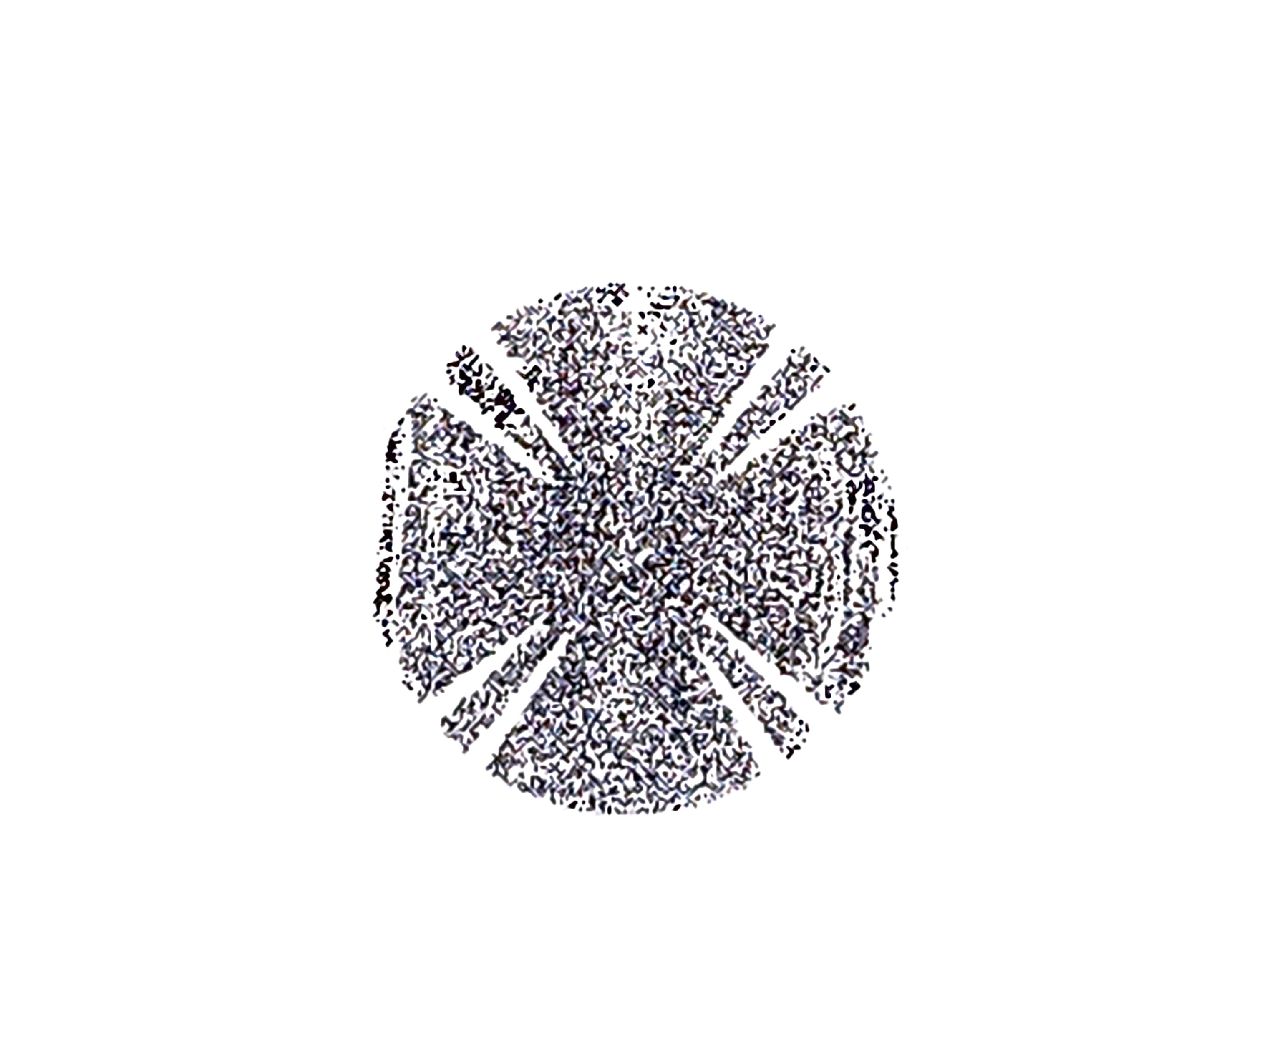
\includegraphics[width=.8\linewidth]{img/slam_1.pdf}
  \caption{全スキャンを同じ位置においた結果\cite{slam:nyumon}}
  \label{slam:scan}
  \end{center}
\end{figure}

\begin{figure}[h]
  \begin{center}
  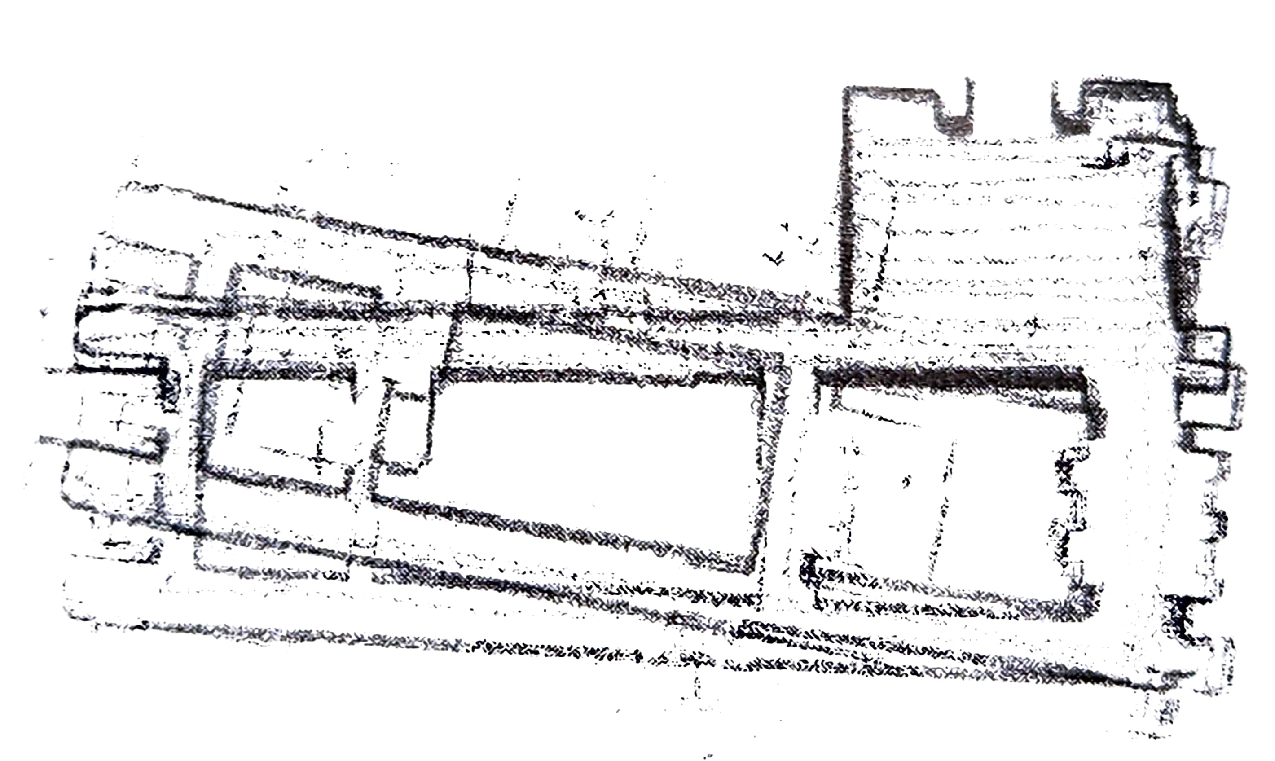
\includegraphics[width=.8\linewidth]{img/slam_2.pdf}
  \caption{オドメトリによる地図\cite{slam:nyumon}}
  \label{slam:odometry}
  \end{center}
\end{figure}

\begin{figure}[h]
  \begin{center}
  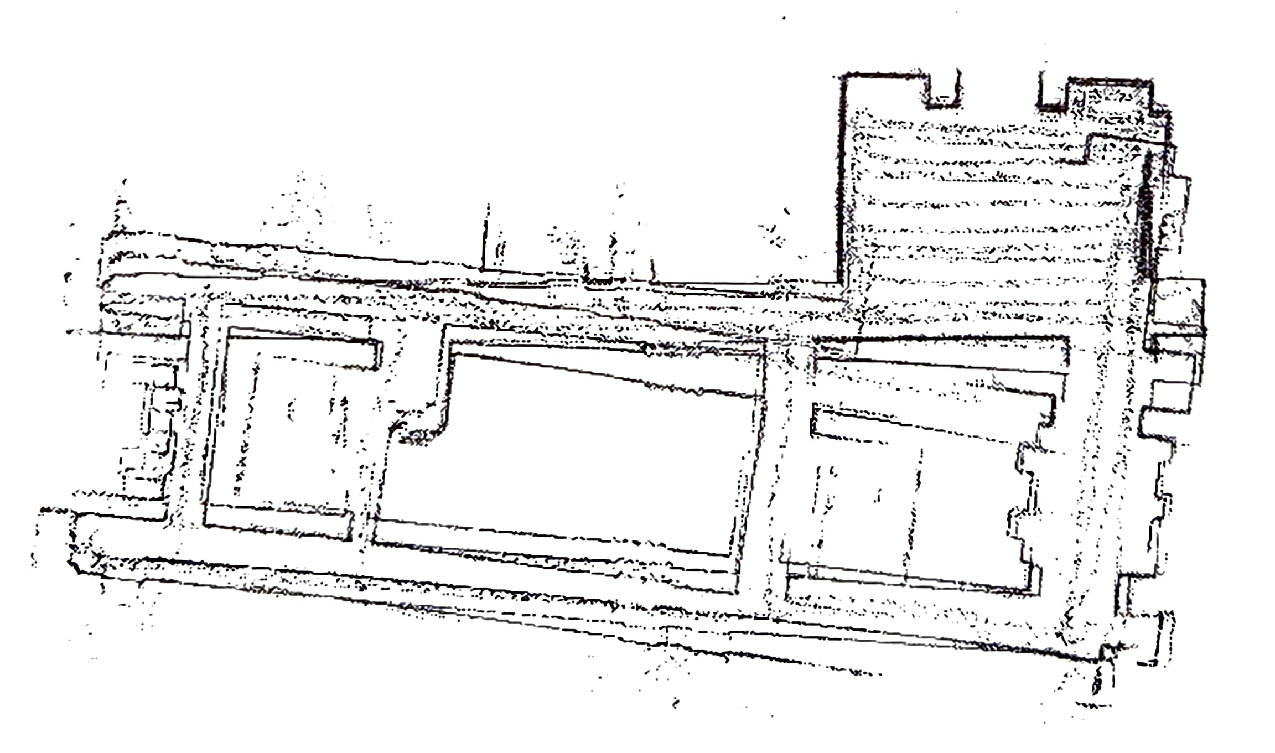
\includegraphics[width=.8\linewidth]{img/slam_3.pdf}
  \caption{SLAMによる地図(ループ閉じ込みなし)\cite{slam:nyumon}}
  \label{slam:slam}
  \end{center}
\end{figure}

\begin{figure}[h]
  \begin{center}
  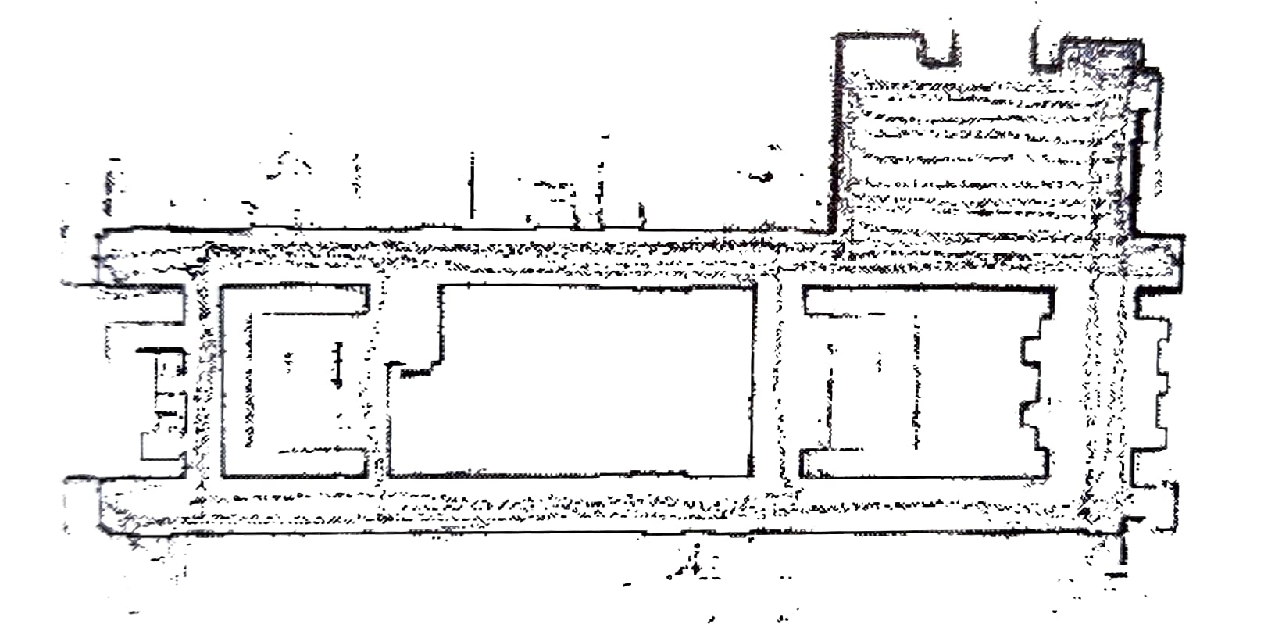
\includegraphics[width=.8\linewidth]{img/slam_4.pdf}
  \caption{SLAMによる地図(ループ閉じ込みあり)\cite{slam:nyumon}}
  \label{slam:slam_loop}
  \end{center}
\end{figure}

SLAMを用いることで、この歪みを減らすことができる。
SLAMには大きくレベルが2段階あり、ループ閉じ込みという技術を用いないレベルでは図\ref{slam:slam}のように局所的なぶれや歪みは小さくなるが、全体的な歪みは残る。
ループ閉じ込みを行うレベルでは図\ref{slam:slam_loop}のように全体形状の歪みも小さくなった地図をえることができる。
このようにSLAMは、ロボット位置と地図の推定を同時に行うことで、地図の精度を向上させる技術である。

\clearpage
\subsubsection{SLAMの実行形態}
SLAMを行う際にまず問題となるのは、センサデータ取得のための走行経路をどのように決めるかである。ロボットは地図を持っていないので、
どういう経路を通るのが安全で効率が良いか、あらかじめ知ることはできない。そこで、以下の2つの方法が考えられる。

\begin{enumerate}
  \item 人間がセンサデータの取得経路を与える\\
  対象環境をよく知っている人間がロボットにセンサデータ取得経路を与える。
  たとえば、人間がロボットを操縦してセンサデータを集める場合がこれにあたる。
  地図の生成は、操縦と同時に行う場合も、データ収集後にオフラインで行う場合もある。
  目的地への自律走行(ナビゲーション)を行う場合は、この方法で地図をつくることが多い。ナビゲーションでは、あらかじめ作成した地図の上で目的地への経路計画と自己位置推定を行うため、その場で地図を作る必要はないからである。
  ただし、ナビゲーションの最中に障害物や環境変化に対処するために、局所的な地図をその場で作って対処することは良くある。
  \item ロボットがセンサデータの取得経路を自律的に決める\\
  ロボットが自律走行してセンサデータを取得しつつ、リアルタイムに地図をつくる。
  その際、それまでに生成した地図と現在地周辺の局所的な地図を自律走行のために使う。ロボットは障害物を回避しながら走行し、次にどこに行くかを自分で決める必要があるため、SLAMだけでなく、探査、経路計画障害物回避なども含んだ総合的なシステムが必要になる。
  このようなシステムは、人間が操縦や遠隔操作をするのが難しい環境、あるいは、地図構築の知識をもったオペレータを用意できないアプリケーションなどで重要になる。理想はロボットが自律で地図を作ることであるが、実用においては目的に応じて使い分ければ良い。
\end{enumerate}

\subsubsection{SLAMの種類}
センサや地図には多くの種類があり、それに応じてSLAMの手法も変わる。
ここではSLAMの大きな分類軸として、2次元か3次元かを考える。
ロボットの位置(運動)と地図が、それぞれ2次元か3次元かで、原理的には4通りの分類ができる。
ここでは、ロボット位置/地図の次元によって、SLAMを2D/2D型、2D/3D型、3D/3D型に分けたものを表\ref{slam:table1}に示す。
(3D/2D型は事例が少ないため除外する。)

\begin{table}[h]
  \centering
  \caption{SLAMの種類}
  \scalebox{.9}{
  \begin{tabular}[t]{cccc}
    \toprule
    &ロボット位置&地図&センサ\\
    2D/2D型&2次元3自由度&2次元&2Dレーザスキャナ、オドメトリ、ジャイロ\\
    2D/3D型&2次元3自由度&3次元&2D/3Dレーザスキャナ、カメラ、オドメトリ、ジャイロ\\
    3D/3D型&3次元6自由度&3次元&3Dレーザスキャナ、カメラ、IMU\\
    \bottomrule
    \label{slam:table1}
  \end{tabular}}
\end{table}

これらのどの型を選ぶかは、ロボットの種類、タスク、コスト等によって変わる。
一般に2D/2D型、2D/3D型、3D/3D型の順に機能が高いと言えるが、コストもかかる機能的には3D/3D型が最も望ましいが、処理量が多いため、多くの場合、高性能コンピュータが必要になる。
ただし、最近は、地図の規模が小さければ、携帯端末レベルのコンピュータでも、3D/3D型SLAMが可能になっている。
移動機能を持ったロボットには、車輪型ロボット、クローラー型ロボット、脚型ロボット、ヒューマノイド、飛行ロボット等がある。
例えば、ヒューマノイドや飛行ロボットのように3次元の運動をするロボットには、3D/3D型が必要である。
車輪型ロボットは、地面や床面等の平面を走ることが多いので、2D/2D型が良く使われている。
ただし、障害物の検出には2D/3D型が有利であり、もし坂道や段差等を考慮するのであれば、車輪型ロボットでも3D/3D型SLAMが必要であると考えられる。

現在のSLAMシステムは、レーザスキャナを使ったものとカメラを使ったものに大別できる。
カメラはさらに、単眼カメラ、ステレオカメラ、距離画像カメラに分かれる。
2D-SLAMはレーザスキャナを用いるものが多く、また、古くから研究がおこなわれていたので、現在では実用レベルになっている。
代表的なものにGmapping\cite{slam:gmapping}やCartographer\cite{slam:cartographer}等がある。
3D-SLAMには、3Dレーザスキャナかカメラ、あるいはその両方が用いられる。

\subsection{SLAMの原理}
SLAMの原理を模式的に述べる。前提として、ロボットに搭載されたセンサのみを使う。
GPSなど、絶対位置が直接得られるセンサや装置は使わない。
簡単のため、ロボットにおけるセンサの設置個所は既知とし、両者の座標系は同一視する。
ロボット位置$\bm{x}$は方向も含めて$(x,y,\theta)^{\mathsf{T}}$ と表す。$x,y$ は、床面等の2次元座標系での位置(並進成分)、$\theta$ はロボットが向いている方向である。
なお、右肩の$\mathsf{T}$は、ベクトルの転置を表す。

\begin{figure}[h]
  \begin{center}
  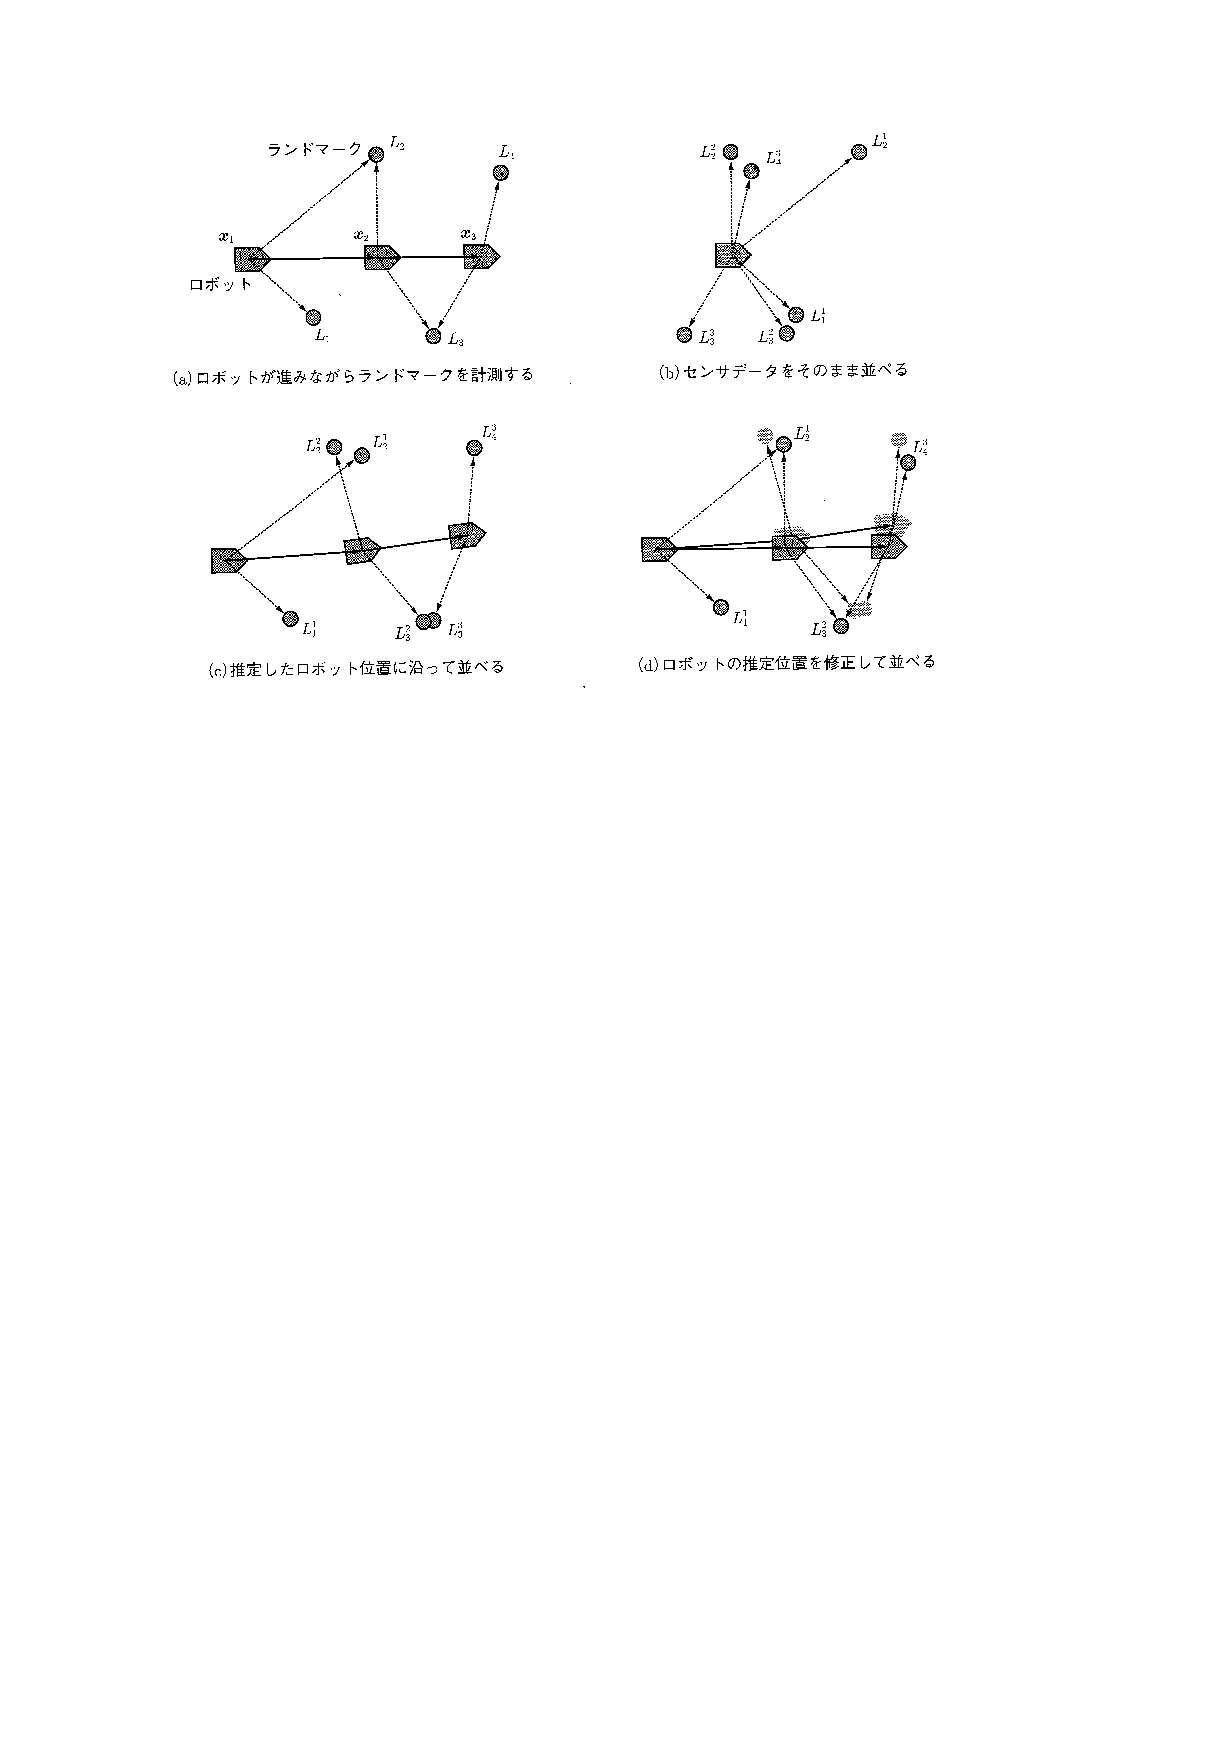
\includegraphics[width=\linewidth]{img/slam_5.pdf}
  \caption{ロボットで地図を作る様子\cite{slam:nyumon}}
  \label{slam:chizu1}
  \end{center}
\end{figure}

図\ref{slam:chizu1}にロボットで地図を作る様子を示す。地図はランドマークだけで構成されているとする。ランドマーク位置は点$\bm{q}$ で表す。
ランドマークに向きはない。この点では点がまばらにあるだけなので、障害物等の形状を表せず、地図としては不十分であるが、ロボットが位置を知るためには使える。
ここでも、ロボットは各ランドマークを区別できると仮定する。

\subsubsection{地図構築:ランドマーク位置の推定}
前述のように、ロボット位置が分かればランドマーク位置は計算できる。図\ref{slam:chizu2}\verb|~|図\ref{slam:suitei}に例を示す。この図では、
図\ref{slam:chizu1}のロボット位置$\bm{x_1}$ からランドマーク$\bm{q_2}$ を見る部分に注目している。$\bm{q_2}$ の地図座標系での位置を
$\bm{q_2}=(q_{2,x},q_{2,y})^{\mathsf{T}}$ また、センサの計測データ(センサ座標系の値)を$\bm{z_2} = (z_{2,x},z_{2,y})^{\mathsf{T}}$とする。
ここで、ロボット位置$\bm{x_1} = (x_1, y_1,\theta_1)^{\mathsf{T}}$ が分かれば、$\bm{q_2}$は式\eqref{slam:eq:q2}のように計算できる。

\begin{figure}[h]
  \begin{center}
  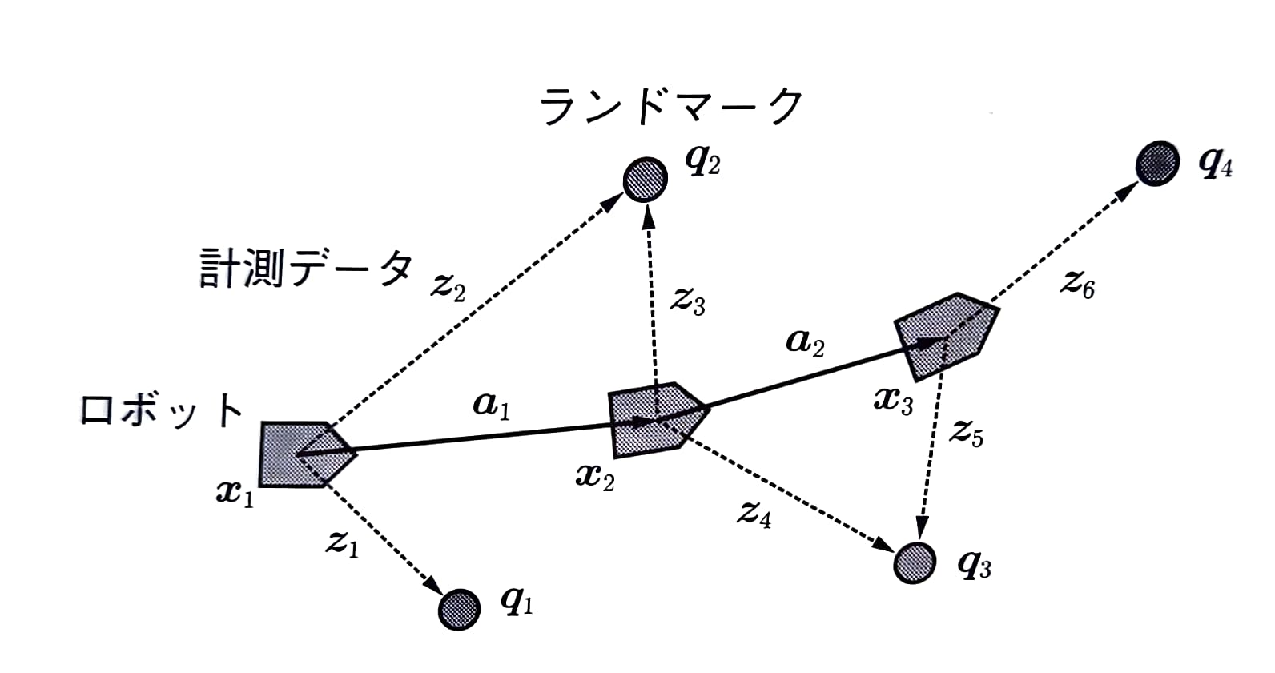
\includegraphics[width=\linewidth]{img/slam_6.pdf}
  \caption{ロボットとランドマークの位置推定\cite{slam:nyumon}}
  \label{slam:chizu2}
  \end{center}
\end{figure}

\begin{figure}[h]
  \begin{center}
  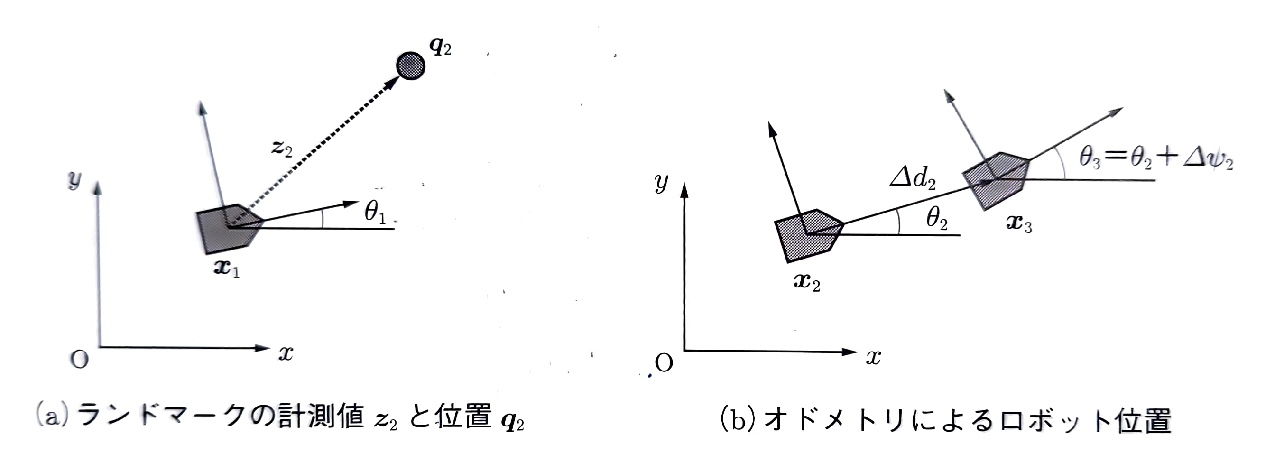
\includegraphics[width=\columnwidth]{img/slam_7.pdf}
  \caption{ランドマーク位置の推定とロボット位置の推定\cite{slam:nyumon}}
  \label{slam:suitei}
  \end{center}
\end{figure}

\clearpage

\begin{align}
  \begin{pmatrix}
    q_{2,x}\\
    q_{2,y}\\
  \end{pmatrix}
  =
  \begin{pmatrix}
    \cos\theta_1&-\sin\theta_1\\
    \sin\theta_1&\cos\theta_1\\
  \end{pmatrix}
  \begin{pmatrix}
    z_{2,x}\\
    z_{2,y}\\
  \end{pmatrix}
  +
  \begin{pmatrix}
    x_1\\
    y_1\\
  \end{pmatrix} \label{slam:eq:q2}
\end{align}

ここで、式を整理すると、
\begin{align}
  \bm{R_1} = 
  \begin{pmatrix}
    \cos\theta_1&-\sin\theta_1\\
    \sin\theta_1&\cos\theta_1\\
  \end{pmatrix},
  \bm{t_1} =
  \begin{pmatrix}
    x_1\\
    y_1\\
  \end{pmatrix}\label{slam:eq:q22}
\end{align}
なお、式\eqref{slam:eq:q22}は、式\eqref{slam:eq:q2f}のように表すことができる。
\begin{align}
  \bm{q_2} = \bm{R_1}\bm{z_2}+\bm{t_1} \label{slam:eq:q2f}
\end{align}

なお、センサがレーザスキャナの場合、センサ中心からランドマークまでの距離$d_2$と方向$\phi$を計測する。
すると、$z_2 = (d_2\cos\phi_2,d_2\sin\phi_2)^{\mathsf{T}}$となる。

\subsubsection{ロボット位置の推定}
ロボット位置を推定する有力な方法の1つにオドメトリ(Odometry)がある。オドメトリは、与えられた初期位置から微小変位を積分して現在位置を求める仕組みである。
例えば、車輪ロボットでは、車輪の回転数から移動量を求める「車輪オドメトリ」が良く用いられる。オドメトリによるロボット位置の計算方法はいくつかあるが、ここでは、
図\ref{slam:suitei}を例に、簡単な方法を紹介する。この図では、図\ref{slam:chizu2}のロボットが$\bm{x_2}$ から$\bm{x_3}$に移動する様子を表している。
オドメトリで得た移動量(ロボット座標系での並進と回転)を$\bm{a_2} = (\Delta d_2,0,\Delta\psi_2)^{\mathsf{T}}$とする。オドメトリで得る移動量は短時間の微小量なので、
瞬間的にはロボットは直進しているとみなし、$y$成分は0にする。すると、ロボット位置は$\bm{x_3}$は次の式\eqref{slam:eq:x3}のように計算できる。

\begin{align}
  \begin{pmatrix}
    x_3\\
    y_3\\
    \theta_3\\
  \end{pmatrix}
  =
  \begin{pmatrix}
    \cos\theta_2&-\sin\theta_2&0\\
    \sin\theta_2&\cos\theta_2&0\\
    0&0&1\\
  \end{pmatrix}
  \begin{pmatrix}
    \Delta d_2\\
    0\\
    \Delta\psi\\
  \end{pmatrix}
  +
  \begin{pmatrix}
    x_2\\
    y_2\\
    \theta_2\\
  \end{pmatrix} \label{slam:eq:x3}
\end{align}

なお、図\ref{slam:chizu2}の$\bm{a_2}$は、微小量である。この計算は、回転成分を含めた座標変換といえるため、compounding演算子$\oplus$で表すことがある。
compounding演算子を用いると、式\eqref{slam:eq:x3}は次のように表すことができる。

\begin{align}
  \bm{x_3} = \bm{x_2}\oplus\bm{a_2}
\end{align}

オドメトリで位置を求めるには、最初に初期位置$x_1$を与え、そこを起点として式\eqref{slam:eq:x3}によって微小な移動量を次々に加算していく。
そうすると、ロボットの位置を時間経過ごとに計算することができる。しかし、オドメトリを移動量を加算していく積分計算なので、移動量に含まれる誤差も加算される。
このため、ロボット位置の誤差が累積してどんどん増えていくという問題がある。そのため、図\ref{slam:odometry}に示すように、オドメトリによる推定位置は走行するにつれてずれていく。
人間に例えると、目をつぶって歩数で距離を推測するようなものであり、歩いているうちに位置がずれる。

\subsubsection{ロボット位置とランドマーク位置の同時推定}
オドメトリには「走行するにつれて誤差が累積する」という問題がある。そのため、図\ref{slam:chizu1}のロボット位置のずれは、これを推定したものである。
この累積誤差を減らすには、センサデータを地図に登録されたランドマークと照合して、ロボット位置を修正する方法が有効的である。目をつぶって歩きながら、時々薄目を開けてランドマークを見て、
自分がどこにいるか確認するようなものである。この時重要なのは、同じランドマークを複数回計測することである。例えば、計測データ$\bm{z_3}$からも、式\eqref{slam:eq:z3}ロボット位置$\bm{x_2}$に関する計算式が得られる。
\begin{align}
  \bm{q_2} = \bm{R_2z_3+t_2} \label{slam:eq:z3}
\end{align}
既に計測したランドマークからロボット位置を逆算して修正するために、式\eqref{slam:eq:q2f}によって$\bm{q_2}$が既知になったと考え、
その$\bm{q_2}$を使って、式\eqref{slam:eq:z3}を用いて$\bm{x_2}$を逆算すれば、ロボット位置を修正できる。ただし、この式だけでは、制約が足りず
逆算できないので、より多くの計算式を立式する。図\ref{slam:chizu2}において、オドメトリとランドマーク計測の計算式を全て立式すると、以下のような連立方程式となる。

\begin{align*}
  \bm{q_1} = \bm{R_1z_1+t_1}\\
  \bm{q_2} = \bm{R_1z_2+t_1}\\
  \bm{q_2} = \bm{R_2z_3+t_2}\\
  \bm{q_3} = \bm{R_2z_4+t_2}\\
  \bm{q_4} = \bm{R_3z_1+t_3}\\
  \bm{x_2} = \bm{x_1\oplus a_1}\\
  \bm{x_3} = \bm{x_2\oplus a_2}\\
\end{align*}

これらの式の変数は、ロボット位置$\bm{x_i}$とランドマーク位置$\bm{q_j}$である。ただし、地図がない時点でロボットの初期位置$\bm{x_1}$は適当な定数(多くの場合、地図座標系の原点)にする。
そのため、変数としてのロボット位置は2個になる。そうすると、ロボット位置は3次元、ランドマーク位置は2次元なので、これらの式の変数は全てで$3\times 2+2\times 4 = 14$個、式は、
$2\times 6+3\times 2=18$個となり、変数より式の方が多い連立方程式となる。変数より式の方が多い連立方程式には、多くの場合、厳密な解が存在しないので、最小二乗法を用いて解くのが一般的である。
ただし、これらの式は非線形関数である三角関数を含むので、非線形最小二乗問題となる。一般的に、センサデータには誤差があり、ロボット位置や地図の推定値にも誤差が波及する。連立方程式を最小二乗問題として解くことは、
推定値の誤差を減らすことにもなる。

\subsubsection{外界センサが一度に大量に得られる場合}
外界センサによる1回の計測で1回の計測で多くのランドマークデータを取得できれば、オドメトリ無しでもロボット位置を決められる。
図\ref{slam:sensor}を例として考える。レーザスキャナやカメラを用いる場合にこれが可能になる。

\begin{figure}[h]
  \begin{center}
  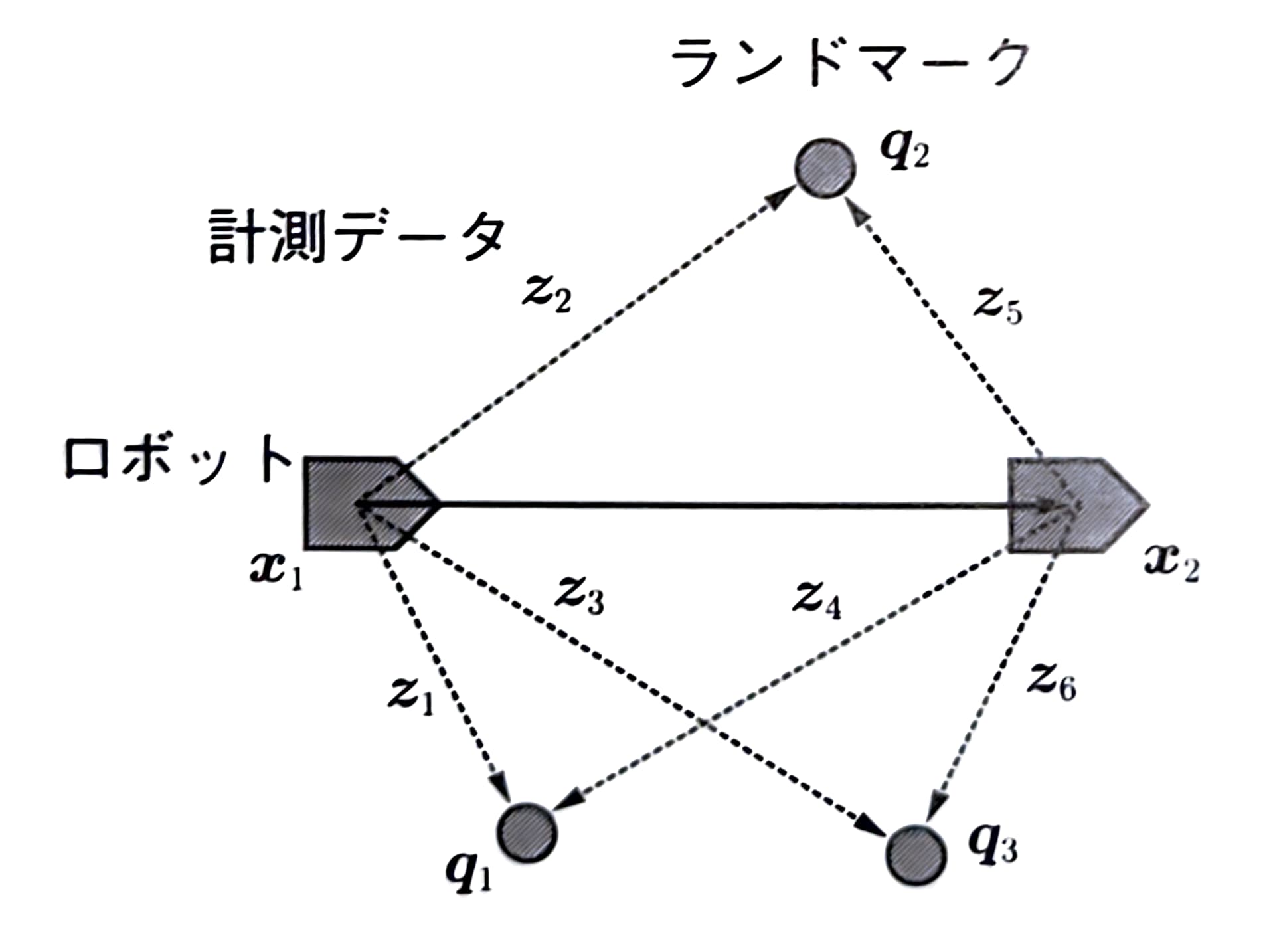
\includegraphics[width=.6\columnwidth]{img/slam_8.pdf}
  \caption{外界センサデータが一度に大量に得られる場合\cite{slam:nyumon}}
  \label{slam:sensor}
  \end{center}
\end{figure}

この図より得られる式は、式\eqref{slam:eq:sensor}に示す。
\begin{align}
  \begin{split}
    \bm{q_1} = \bm{R_1z_1+t_1}\\
    \bm{q_2} = \bm{R_1z_2+t_1}\\
    \bm{q_2} = \bm{R_1z_3+t_1}\\
    \bm{q_3} = \bm{R_2z_4+t_2}\\
    \bm{q_3} = \bm{R_3z_5+t_2}\\
    \bm{q_4} = \bm{R_3z_6+t_2} \label{slam:eq:sensor}
  \end{split}
\end{align}

ロボット位置は3次元、ランドマーク位置は2次元なので、これらの式の変数は全部で$3\times1+2\times3=9$個、式は
$2\times6 = 12$個となる。変数より式の方が多いので、前と同様に最小二乗法により解を求めることができる。この連立方程式にはオドメトリの制約が含まれていないが、
このように外界センサデータだけでロボット位置を求めることができる。上記の例はランドマークまでの距離と方向を計測できるレーザスキャナを用いた場合である。レーザスキャナのデータだけからロボット位置を求める方法には、例えば「スキャンマッチング」が挙げられる。

\subsection{要素技術}
ここではSLAMで必要となる要素技術について説明する。具体的にはこれまでの原理を実現する方法について述べる。

\subsubsection{不確実性の扱い}
センサデータには多くの誤差が含まれており、自己位置推定や地図構築に不確実性をもたらす。ここでは、偶然誤差の扱い方について述べる。偶然誤差はランダムに発生する確率で、
原因が特定できないため、確率的に扱う必要がある。前節の連立方程式には誤差が明示的に考慮されておらず、方程式自体はいわば誤差の無い理想的な状態を表しているが、現実ではそうはならない。
そこで、不確実性を扱うために、誤差を明示的に表す。式\eqref{slam:eq:q2f}を再喝する。
\begin{align*}
  \bm{q_2} = \bm{R_1z_2+t_1}
\end{align*}
これを次のように変形して、ロボット(センサ)座標系で見たランドマーク位置を考える。
\begin{align}
  \bm{z_2} = \bm{R_1^{-1}(q_2-t_1)}\eqdef \bm{h(x_1},\bm{q_2)}
\end{align}

ここで、$\eqdef$は定義を表す。$\bm{z_2}$は、実際の計測値、$\bm{h}$は、ロボット(センサ)座標系でのランドマーク位置を計算する関数である。
この式では等号を結んでいるが、実際は計測値$\bm{z_2}$に誤差があるため左の等式は成り立たない。そこで誤差を導入する。誤差は計測値と真値の差である。$\bm{x_1}$と$\bm{q_2}$は変数であるが、一旦それらを真値とみなすと、$\bm{z_2}$の誤差$\bm{v_2}$は次のようになる。
\begin{align}
  \bm{v_2} = \bm{z_2}-\bm{h(x_1},\bm{q_2)}
\end{align}

多くの誤差は正規分布に従うことで知られており、SLAMでも正規分布が最もよく使われる。そこで、ここでの誤差$v_2$も正規分布に従うと仮定することにする。
正規分布は平均と分散(多次元の場合は共分散行列)の2つのパラメータで定義できるので、$\bm{v_2}$も正規分布に従うと仮定する。正規分布は平均と分散(多次元の場合は共分散行列)の2つのパラメータで定義できるので、
$\bm{v_2}$の平均を$\bm{\mu_2}$、共分散行列を$\Sigma_2$とすると、$\bm{v_2}$は式\eqref{slam:eq:keisoku}の正規分布で表される。

\begin{align}
  p(\bm{v_2}) =\frac{1}{\sqrt{|2\pi\Sigma_2|}}\exp\biggl\{-\frac{1}{2}(\bm{v_2}-\bm{\mu_2})^{\rm{T}}\Sigma_2^{-1}(\bm{v_2-\mu_2})\biggr\}
\end{align}

\begin{align}
  p(\bm{v_2}) =\frac{1}{\sqrt{|2\pi\Sigma_2|}}\exp\biggl\{-\frac{1}{2}(\bm{z_2}-\bm{h}(\bm{x_1},\bm{q_2}))^{\rm{T}}\Sigma_2^{-1}(\bm{z_2}-\bm{h}(\bm{x_1},\bm{q_2}))\biggr\}\label{slam:eq:keisoku}
\end{align}

これを計測モデル(観測モデル)という。オドメトリの誤差も同様に式\eqref{slam:eq:x3}を例にすると、関数$\bm{g}$を使って、次のように表す。
\begin{align*}
  \bm{x_3} = \bm{x_2}\oplus \bm{a_2} \eqdef \bm{g}(\bm{x_2},\bm{a_2})
\end{align*}

これに、誤差$\bm{u_2}$を導入し、次のように表す。
\begin{align*}
  \bm{u_2} = \bm{x_3}-\bm{g}(\bm{x_2,a_2})
\end{align*}

上と同様に、誤差$\bm{u_2}$を導入して、式\eqref{slam:eq:undou}のように表す。
\begin{align}
  p(\bm{u_2}) = \frac{1}{\sqrt{|2\pi\Sigma_3|}}\exp\biggl\{-\frac{1}{2}(\bm{x_3}-\bm{g}(\bm{x_2},\bm{a_2}))^{\rm{T}}\Sigma_2^{-1}(\bm{x_3}-\bm{g}(\bm{x_2},\bm{a_2}))\biggr\} \label{slam:eq:undou}
\end{align}
と表す。これを運動モデルと呼ぶ。前の連立方程式の全誤差の確率密度$p$は、$u_i, v_j$の確率密度$p$を掛け合わせたものになる。

\begin{align}
  p = \prod_{i=1}^{2}p(\bm{u_i})\prod_{j=1}^{6}p(\bm{v_i})
\end{align}

この式はSLAMの構造を完全に表しており、この確率密度$p$を推定する問題は完全SLAM問題と呼ばれている。
この式は、最終的には、非線形最小二乗問題に帰着される。

\subsubsection{データ対応付け}
データ対応付け(data association)とは、「別々に計画されたセンサデータで、同じものを対応づけること」である。
SLAMでは、とくに、現在計測したセンサデータと、地図に登録されたランドマークの対応付けが重要になる。
「ロボットはランドマークを区別できる」という前提でSLAMの原理を説明した。
例えば、ICタグやビーコン等でID(識別子)が付いたランドマークであれば、IDをもとに一意に区別することが可能である。
このような装置を用いてロボットが場所や物体を認識する研究もなされており、目的・応用によっては非常に有効である。
一方SLAMでは、もともと存在する地形・風景・物体等を(IDのない)ランドマークとして用いることがよく行われている。
IDの無いランドマークを区別してデータ対応付けを行うのは、そう簡単ではない。
IDに変わる手がかりとして、ランドマーク位置と特徴量がよく使われる。

\begin{enumerate}
  \item 位置制約による対応づけ\\
  自己位置がある程度の精度で推定できるならば、その周辺の地図に登録されたランドマーク位置も予測できる。
  「自分は今地点Aにいるので、この方向にランドマークBが存在するはず」という具合である。そうすると、周辺のランドマーク位置を予想して、
  現在取得したセンサデータに最も近いものを対応づけるという方法が考え付く。非常によく用いられる。
  \item 特徴量による対応づけ\\
  センサデータとランドマークになんらかの特徴量を付加して、その特徴量によって両者の対応付けを行う方法である。特徴量はセンサによって多種多様で、
  レーザスキャンなら局所記述子やレーザの反射強度、カメラ画像ならば局所記述子や少領域の色・形状等がある。強力な特徴量ならば、それだけでかなりの対応づけができる。
  単純な特徴量では、それだけで対応づけるのは難しいが、候補の絞り込みに使うことができる。
\end{enumerate}

一般には、位置制約だけで対応付けを行うのは十分ではない。同じぐらいの位置に2つのランドマークがあった時に、どちらに対応づけるのが良いか判断するのが難しいからである。
逆に、特報量を用いる場合も、それだけで対応付けを完結するのは危険である。形状や外見が良く似たランドマークは区別が難しいからである。このため、特徴量を用いて対応候補を減らした上で
位置の探索範囲が狭く、しかも、一度に多くのセンサデータを計測できる場合は、位置制約だけで対応づけが上手くいく可能性が高くなる。
探索範囲が狭いために、対応付けの候補が少なく、しかも、同時に計測したデータ間の位置制約も使えるからである。「スキャンマッチング」という手法では、この性質を利用する。

\subsubsection{センサ融合}
前のように、大量データを一度に取得できる外界センサがあれば、基本的には、オドメトリ無しでSLAMを行うことが可能である。
しかし、実際には、そのような外界センサを用いても状況によっては大量データを得られないことがあり、センサデータに十分な情報が含まれていない場合もある。例えば、極端な場合、センサデータにランドマークが1つも含まれていない場合もある。
センサデータにランドマークが1つも含まれていなければ、ロボット位置は推定できない。この場合は、オドメトリを使うしか方法はない。さらにセンサデータは取れているが、情報が不足している場合等が考えられる。オドメトリを使わない場合、一度に得たセンサデータにランドマークが1個しか含まれていなければ、それだけではロボット位置を確定できない。前節でのSLAMの定式化では、オドメトリを用いていたので、ランドマークが1個でも、連立方程式の一部として、ロボット位置の推定に活かすことができた。しかし、オドメトリを使わない場合、センサデータにランドマークが1個しか含まれないとロボット位置は不定になってしまう。
例えば、式\eqref{slam:eq:q2}では、ロボット位置が変数3個に対して、方程式は2個しかないので、解は不定になる。
一般には、センサデータにランドマークが多く含まれているほど、安定して解が得られる。
ところが、センサデータにランドマークが多数含まれても、上手くいかない場合がある。
例えば、長い廊下にロボットがいる場合を考えてみる。
今、外界センサによって壁を計測してロボット位置を推定することを考える。
廊下の2つの壁は平行なので、その地図は計測点が2本の平行な直線上に並んだようになる。
同様に、センサデータも2本の平行な直線になる。壁に模様がないと仮定すると、この2本の直線を使ってロボット位置を一意に確定することはできない。
地図とセンサデータは、これらの直線に垂直な方向には位置が決まるが、平行な方向にはどこの位置でも合うからである。
このような状況を退化という。このように一度に大量のデータを計測できるセンサを用いたとしても、状況によっては情報が不足することがあり、ロボット位置を確定できなくなる。
このため、ロボットが安定して動作するためには、1つの外界センサだけでなく、オドメトリのような他のセンサを併用することが重要である。

\subsubsection{ループ閉じ込み}
SLAMにおいて重要な概念にループがある。図\ref{slam:loop_kiseki}にロボットの軌跡のループを示す。
ループとは周回路のことで、以前通った場所を再び通る経路である。SLAMによってランドマークを複数回計測してオドメトリによるロボット位置の累積誤差を減らした。これによって累積誤差は減るが、完全には消せない。
それは、ランドマーク計測にも誤差があるからである。ランドマーク位置が外部からあたえられたもの(既存地図など)であれば、誤差は累積しない。しかし、SLAMにおいては、ランドマーク位置も自分で推定したものなので、
ランドマーク位置に誤差が入り、そのランドマークを基準に自己位置すいていするとまた誤差が生じて、というように、誤差は累積していく。
SLAMでロボット位置の累積誤差をオドメトリ単体の場合よりも減らせるのは、その誤差の増加が、たいていはオドメトリ単体の場合より小さいからである。

\begin{figure}[h]
  \begin{center}
  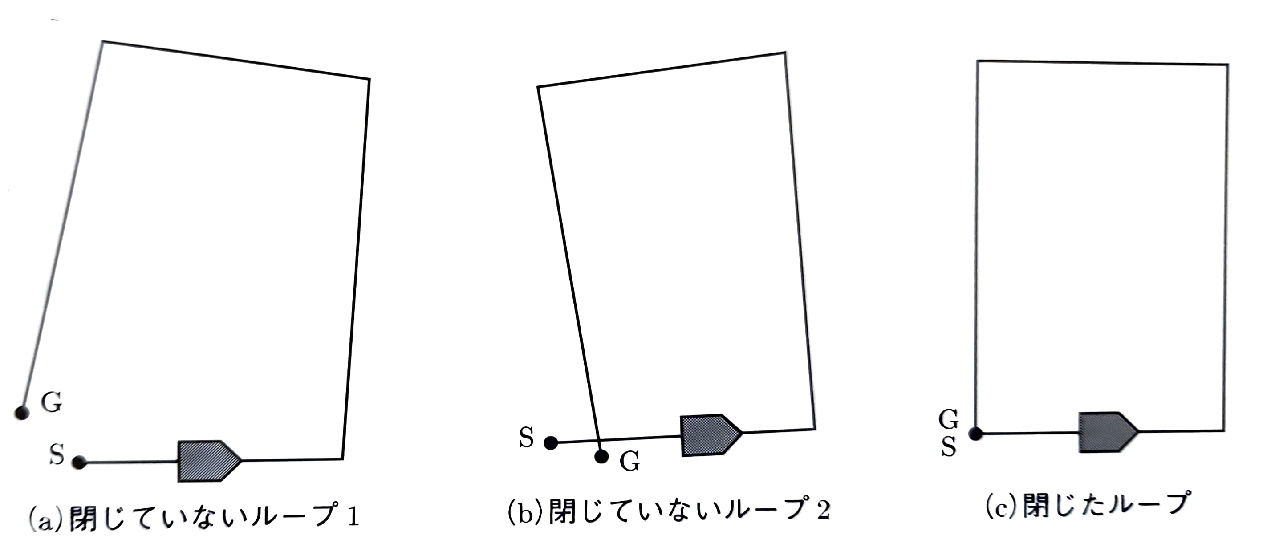
\includegraphics[width=.8\linewidth]{img/slam_9.pdf}
  \caption{ロボットの軌跡のループ\cite{slam:nyumon}}
  \label{slam:loop_kiseki}
  \end{center}
\end{figure}

このように、SLAMにも累積誤差があるので、ループは多くの場合、閉じない。図\ref{slam:loop_kiseki}に例を示す。
ロボットはS(スタート)から出発して1周し、Sと同じ位置にあるG(ゴール)に行くとする。この図で(a)は開いてしまった例、
(b)は重なってしまった例である。このように地図が歪んで実世界との違いが大きくなれば、ロボットが壁や障害物に衝突するかもしれない。
さらに困るのは、地図が歪んで実世界との違いが大きくなれば、ロボットが壁や障害物に衝突するかもしれない。さらに困るのは、地図が歪んで経路の接続関係が変わることである。
たとえば、経路がつながらなかったり、偽の交差点ができたりすると目的地までの経路を上手く見つけられなくなる。このため、ループを閉じることがSLAMの重要な処理になる。
これをループ閉じ込みという。(c)が、ループが閉じ状態である。ループ閉じ込みは次の手順で行う。

\begin{enumerate}
  \item ループ検出\\
  ロボットが同じ場所に戻ったことを検出する。ただし、まったく同じ座標に戻ることはめったになく、たいていは少しずれる。
  図\ref{slam:loop_detect}にループ閉じ込みの様子を示す。(a)は、ループがまだ閉じていない状態である。位置$\bm{x_k}$で、$\bm{x_1}$と同じランドマーク
  $\bm{q_1},\bm{q_2}$を計測したとする。$\bm{x_k}$は誤差によりずれているので、それにもとづいて配置したランドマーク位置$\bm{q_1^{\prime}},\bm{q_2^{\prime}}$もずれている。
  しかし、本来は同じランドマークなので、$\bm{q_1^{\prime}},\bm{q_2^{\prime}}$と、$\bm{q_1},\bm{q_2}$が同じになるようなロボットの位置
  $\hat{\bm{x_k}}$を求める。(a)ではループは閉じておらず、本来同じはずのランドマーク$\bm{q_1^{\prime}},\bm{q_2^{\prime}}$と、$\bm{q_1},\bm{q_2}$がずれている。(b)ではループ閉じ込み
  により正しいロボット位置$\hat{\bm{x_k}}$を見つけ、$\bm{q_1^{\prime}},\bm{q_2^{\prime}}$は、$\bm{q_1},\bm{q_2}$と一致している。
  
  \begin{figure}[h]
    \begin{center}
    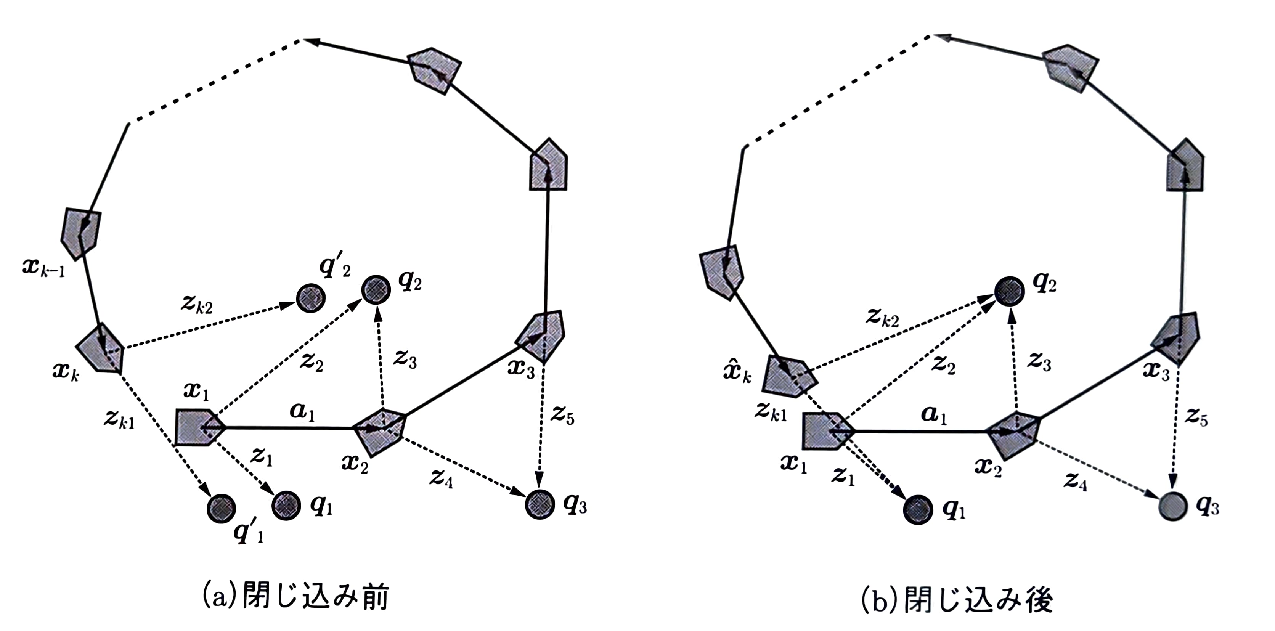
\includegraphics[width=.8\linewidth]{img/slam_10.pdf}
    \caption{ループ閉じ込みの様子\cite{slam:nyumon}}
    \label{slam:loop_detect}
    \end{center}
  \end{figure}
  \item ロボット軌跡と地図の修正\\
  図\ref{slam:loop_detect}で、ループを閉じると、$\bm{x_k}$は、$\hat{\bm{x_k}}$の位置に来るはずである。しかしそうすると、$\hat{\bm{x_k}}$と$\bm{x_{k-1}}$のずれが大きくなってしまうので、
  $\bm{x_{k-1}}$のずれが大きくなってしまうので、$\bm{x_{k-1}}$も修正する。こうして、逆向きにロボットの位置を修正していく。これに伴い、各ロボット位置で計測したランドマーク位置も修正する。
\end{enumerate}

この手順に従うと、軌跡を逆向きに修正していくことになるが、より効率的で精度が良いのは、連立方程式を一度に解くことである。ループ閉じ込みは、上で述べたSLAMの累積誤差を解消するのに有効である。ループが大きい程累積誤差は大きくなるので、それをループ閉じ込みで解消すれば、大きな誤差が一気に修正されたことになる。
以上の通り、ループ閉じ込みはSLAMの重要な要素技術であり、多くの研究が行われてきた背景にある。

\subsection{SLAMの処理形態:一括処理と逐次処理}
SLAMを連立方程式として考えると、センサデータを十分にそろえて、多くの方程式を立てた上で、一括で計算することになる。
前述の完全SLAM問題やループ閉じ込みは、基本的には一括処理である。
人間がロボットを操縦してセンサデータを集める場合は、このような一括処理で地図を作ることができる。
一方、ロボットが走行している最中に地図を作りたいことも良くある。
ロボットが自律的にセンサデータを集める場合は、センサデータを集めている最中にも地図が必要になる。
また、既存の地図を用いてナビゲーションを行っている場合でも、地図構築時とは環境が変化している可能性があるため、安全のために周囲の局所地図をリアルタイムで作り続けることが重要である。
このような場合は、連立方程式が全てそろうのを待たずに、それまでに収集された小数のセンサデータで作った部分的な連立方程式を解いて、逐次的に地図を構築していくことになる。
逐次的な地図構築は前節で述べたように、ロボット位置と地図を交互に求めていくことで行う。
すなわち、時刻$t-1$の地図に統合して、地図$t$の地図を求める。以上のように、SLAMの実行形態には、一括処理と逐次処理が考えられる。
それぞれの特徴を以下に示す。

\begin{enumerate}
  \item 一括処理の特徴
  \begin{itemize}
    \item センサデータが十分多く揃ってから行うため、リアルタイム処理に向かない。
    \item 多くのセンサデータを用いるので、処理時間は長いが、地図の精度は良い。
  \end{itemize}
  \item 逐次処理の特徴
  \begin{itemize}
    \item リアルタイムで逐次的に地図を構築する。このため、未知環境や変化する環境で行動する場合に有用である。
    \item 一部のセンサデータしか用いないので、処理時間は短いが、地図の精度は高くない。
  \end{itemize}
\end{enumerate}

なお、一括処理においても、必ずしも全センサデータがそろっている必要はない。十分多くのセンサデータがあれば、一括処理する意味がある。
実用上の一つの区切りは、ループを見つけるまでである。このように、両者は補完し合う性質を持つため、組み合わせて使うのが望ましい。

\subsection{Gmapping}
ここでは、SLAMの実証例であるGmappingについて述べる。
Gmappingのアルゴリズムは、Rao-Blackwellized Particle Filter (RBPF)によるGrid-Based SLAMである。
RBPFはベイズフィルタ系のパーティクルフィルタ(PF)の一種であり、SLAMにおいては、ロボット位置をPFで、地図を他の何らかのフィルタで推定するものと捉える。
ここでは、各パーティクルが現在のロボット位置だけでなく過去の走行軌跡も保持できる性質を利用している。
すなわち、パーティクルごとの走行軌跡に基づいて、各パーティクルで独立に地図を推定する。
パーティクルの数だけ、地図の仮説、ここでは占有格子地図が生成される。
占有格子地図の推定にはバイナリベイズフィルタによって、確率的に求められる。
Gmappingは、文献\cite{slam:gmapping}に示された格子ベースFast SLAMを実装したものである。以下にFastSLAMの流れを示す。

\begin{enumerate}
  \item 事前推定
  \begin{itemize}
    \item 動作モデルに従ってサンプリング
    \item 観測に従ってサンプルを更新(作成途中の地図情報を利用)
  \end{itemize}
  \item 観測更新1
  \begin{itemize}
    \item 重みを計算
  \end{itemize}
  \item 地図更新
  \begin{itemize}
    \item 地図を更新する(事前推定による状態値を利用)
  \end{itemize}
  \item 観測更新2
  \begin{itemize}
    \item 重みが最大となる粒子の状態値と地図を現時刻の推定値とする。
    \item 必要ならリサンプリングする。
  \end{itemize}
\end{enumerate}

なお、FastSLAMにも1.0と2.0が存在し、GmappingではFastSLAM2.0が実装されている。FastSLAMの流れについて、FastSLAM1.0から述べる。
前提として時刻$t$でロボットが移動している。今使える地図は、時刻$t-1$までに作成された中途半端なものである。この状態でロボットの位置と地図を更新することを考える。
図\ref{slam:zentei}に各々の時刻で作成された地図を示す。

\begin{figure}[h]
  \begin{center}
  \subfigure[時刻$t$までに作成された地図]{
  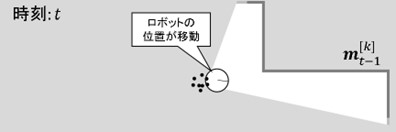
\includegraphics[width=.8\columnwidth]{img/slam_11.jpg}
  \label{slam:zentei1}
  }
  \subfigure[時刻$t-1$までに作成された地図]{
  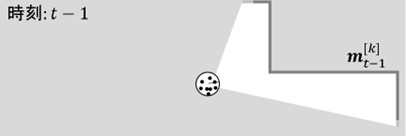
\includegraphics[width=.8\columnwidth]{img/slam_12.jpg}
  \label{slam:zentei2}
  }
  \caption{各時刻において作成された地図}
  \label{slam:zentei}
  \end{center}
\end{figure}

\subsubsection{事前推定}
今の時刻フレームでの地図を作成する前に、ロボットの動作モデル(制御指令に対する応答の予測体系:オドメトリ等)に従って、
今の時刻フレームにおける自己位置の候補点(位置と姿勢)に粒子を撒き、粒子の観測を行う。
動作モデルがホイールオドメトリならば、あらかじめホイールオドメトリに生じる誤差とその確率が明らかであれば、
それに従って点の撒き方が決定される。図\ref{slam:sample}にサンプルの撒き方の決定を示す。

\begin{figure}[h]
  \begin{center}
  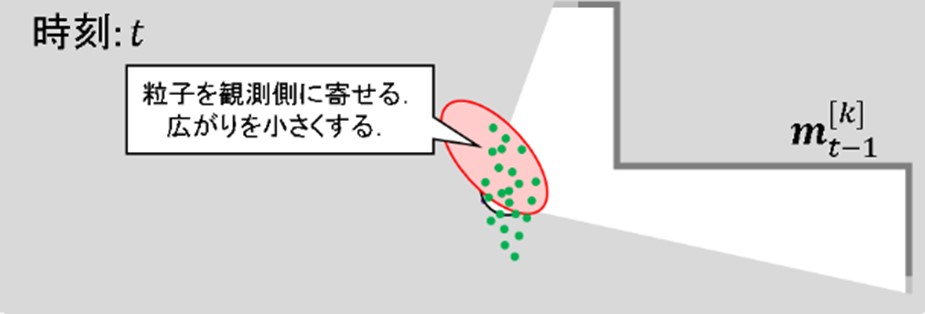
\includegraphics[width=.8\linewidth]{img/slam_13.jpg}
  \caption{サンプルの撒き方の決定}
  \label{slam:sample}
  \end{center}
\end{figure}

\subsubsection{観測更新1}
事前推定において撒いた各候補点から、既知の地図を観測した場合にどのように見えるかという予測と、
現在センサの実観測値を照合し、各候補点の尤度を計算し、各粒子の重みを更新する。図\ref{slam:sample_omomi}、\ref{slam:sample_yuudo}
に、尤度による重みの調整と事前推定を考慮した尤度の調整を示す。

\begin{figure}[h]
  \begin{center}
  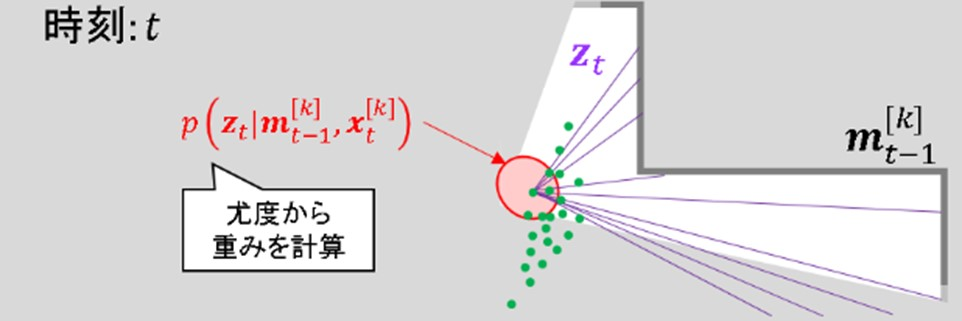
\includegraphics[width=.8\linewidth]{img/slam_14.jpg}
  \caption{尤度による重みの計算}
  \label{slam:sample_omomi}
  \end{center}
\end{figure}

\begin{figure}[h]
  \begin{center}
  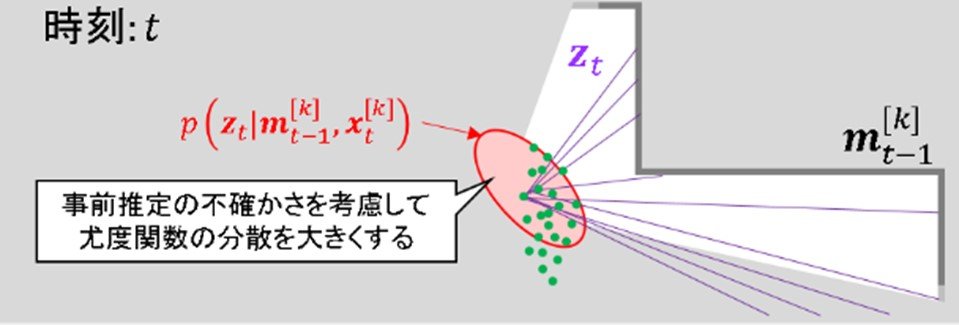
\includegraphics[width=.8\linewidth]{img/slam_15.jpg}
  \caption{事前推定を考慮した尤度の調整}
  \label{slam:sample_yuudo}
  \end{center}
\end{figure}

\subsubsection{地図更新}
各候補点それぞれを自己位置・姿勢であると仮定して、リサンプリングの前に地図を更新する。
図\ref{slam:sample_jikoichi}、\ref{slam:sample_chizu_koushin}に自己位置の仮定と、地図の更新を示す。

\begin{figure}[h]
  \begin{center}
  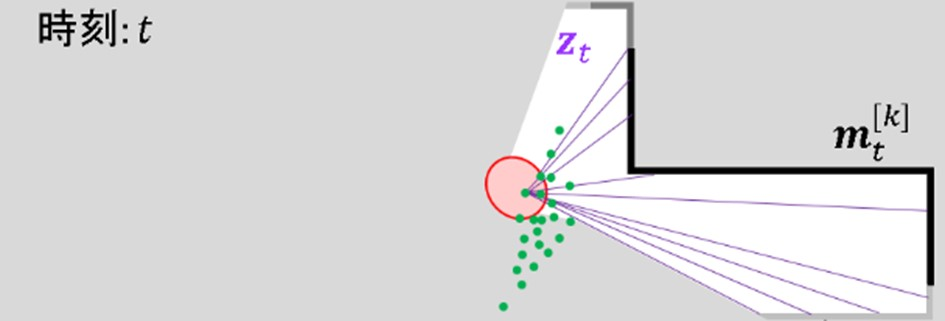
\includegraphics[width=.8\linewidth]{img/slam_16.jpg}
  \caption{自己位置の仮定}
  \label{slam:sample_jikoichi}
  \end{center}
\end{figure}

\begin{figure}[h]
  \begin{center}
  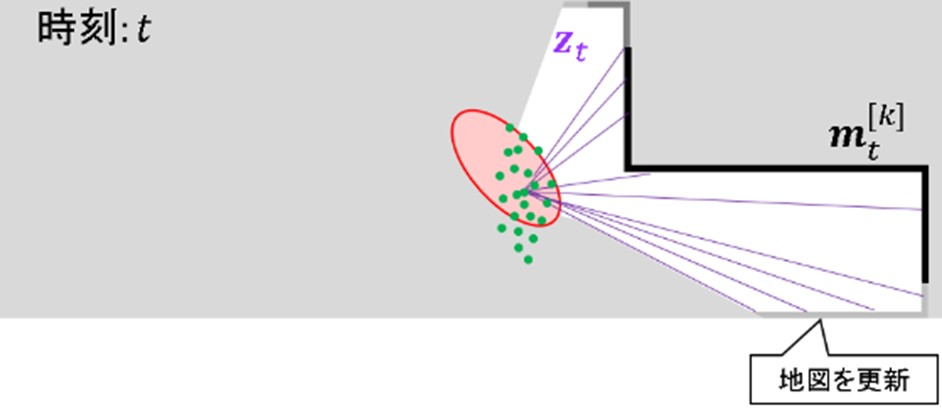
\includegraphics[width=.8\linewidth]{img/slam_17.jpg}
  \caption{地図の更新}
  \label{slam:sample_chizu_koushin}
  \end{center}
\end{figure}

\subsubsection{観測更新2}
地図を更新した後に、現時刻の推定値を確定する。最終的に、各候補点から「重みが最大」の粒子を選択し、
現在における自己位置推定結果として確定する。図\ref{slam:sample_suitei_kakutei}に自己位置推定結果の確定を示す。
また、図\ref{slam:sample_resampling}、\ref{slam:sample_tayou}に、粒子のサンプリングと粒子の多様性の考慮を示す。

\begin{figure}[h]
  \begin{center}
  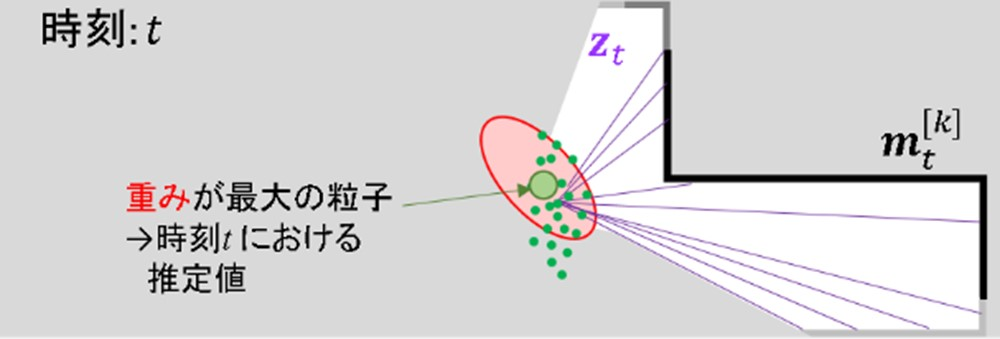
\includegraphics[width=.8\linewidth]{img/slam_18.jpg}
  \caption{自己位置推定結果の確定}
  \label{slam:sample_suitei_kakutei}
  \end{center}
\end{figure}

\begin{figure}[h]
  \begin{center}
  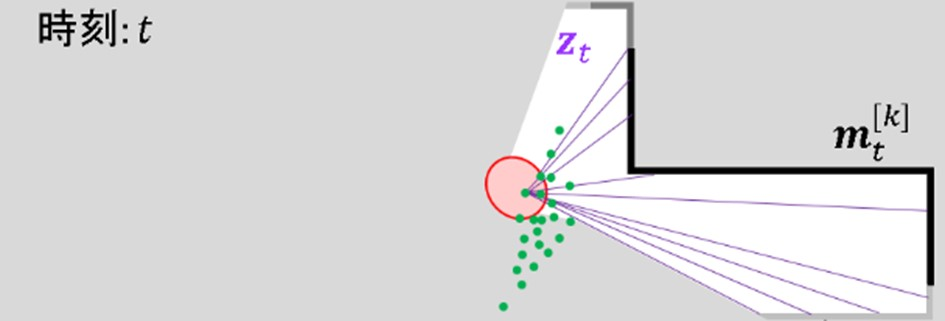
\includegraphics[width=.8\linewidth]{img/slam_19.jpg}
  \caption{粒子のリサンプリング}
  \label{slam:sample_resampling}
  \end{center}
\end{figure}

\begin{figure}[h]
  \begin{center}
  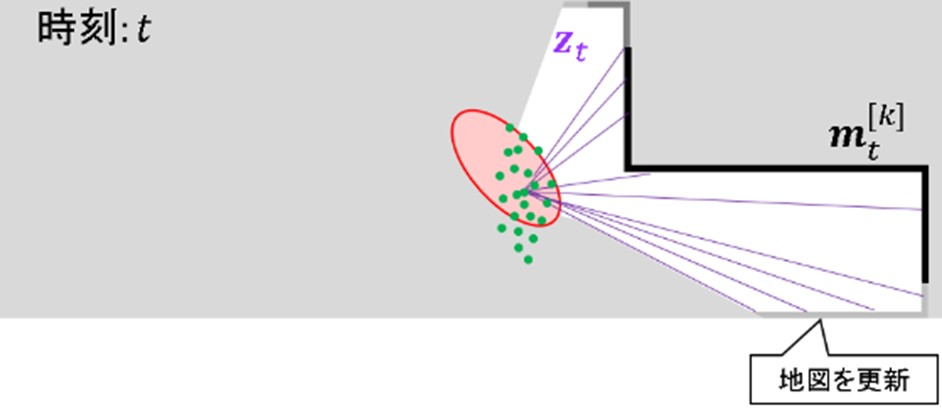
\includegraphics[width=.8\linewidth]{img/slam_20.jpg}
  \caption{粒子の多様性の考慮}
  \label{slam:sample_tayou}
  \end{center}
\end{figure}

\clearpage
\subsection{Hector SLAM}
ここでは、SLAMの実装例であるHector SLAMについて述べる。Hector SLAMは、スキャンマッチングで環境地図を構築している。
スキャンマッチングは、LiDARから刻々と得られる測定データを逐次重ね合わせていき、その際に生じる測定データの移動量からロボットの移動量を推定する手法である。
なお、スキャンマッチングに良く用いられる手法がICP(Iterative Closest Point)アルゴリズム\cite{slam:masuda}, \cite{slam:icp}である。Hector SLAMの場合も環境地図の構築に
ICPアルゴリズムの手法を取り入れている。Hector SLAMの場合、Gauss-Newton法で最適化を行い、最適されたものを式\eqref{slam:hector1}で剛体変換している。

\begin{align}
  \xi^{*} = \arg\min\sum_{i = 1}^{n} \left[1-\rm{M}(\rm{\bm{S}}_i(\bm{\xi}))\right]^2 \label{slam:hector1}
\end{align}

ここで、$\xi=(p_x,p_y,\psi)^{\rm{T}}$と、$\rm{\bm{S}}_i(\bm{\xi})$は、グローバル座標系におけるスキャンされた測定データ$i$の端点を表し、
ある連続したマップの座標$P_m$における占有値$\rm{M}(P_m)$は、サブ占有格子の精度を与えるためにバイリニアフィルタリングを用いて計算される。
式\ref{slam:eq:gauss}は、Gauss-Newton法を用いた$\Delta\xi$についての最小化させる式を表し、式\eqref{slam:eq:hesse}はそのヘッセ行列である。式\eqref{slam:eq:gauss}、\eqref{slam:eq:hesse}
は、占有値$\rm{M}(P_m)$すなわち、ある座標$P_m$におけるマップ勾配に依存する。

\begin{align}
  \Delta\xi = \rm{H}^{-1}\sum_{i = 1}^{n}\Biggl[\nabla M(S_i(\bm{\xi}))\frac{\partial\rm{S}_i(\bm{\xi})}{\partial\bm{\xi}}\Biggr]^{\rm{T}}[1-M(\rm{S}_i(\bm{\xi}))] \label{slam:eq:gauss}
\end{align}

\begin{align}
  \rm{H} = \Biggl[\nabla M(S_i(\bm{\xi}))\frac{\partial\rm{S}_i(\bm{\xi})}{\partial\xi}\Biggr]\Biggl[\nabla M(S_i(\bm{\xi}))\frac{\partial\bm{S}_i(\xi)}{\partial\bm{\xi}}\Biggr] \label{slam:eq:hesse}
\end{align}

\subsection{Cartographer}
Cartographerは、グリッドベースのスキャンマッチングによる逐次SLAMと一括処理のグラフベースSLAMの二種類で構成されている。
スキャンマッチングは、2Dの占有格子地図(Occupancy Grid Map)と、2D-LiDARから取得したスキャンデータを重ね合わせてロボットの自己位置を推定する処理である。
占有格子地図とは、環境を格子状に区切って、それぞれの格子に障害物が存在する確率(占有確率)を割り当てるものである。
例えば、黒い格子ほど占有確率が1に近く、白い格子ほど占有確率が0に近くなる。
また、LiDARは、センサから周囲の環境に向けてレーザ光を照射し、その反射光を受光素子で検知することで、センサから見た障害物までの距離と方向を取得する。
レーザ光が障害物に当たって跳ね返り、センサ中心まで戻ってくるまでの時間を計測することで、障害物までの距離を計算できる。
LiDARセンサが回転しながら、あらゆる方向に対レーザ光を照射するので、周囲の様々な障害物までの、距離と方向のペアが幾つも得られる。
LiDARセンサ1周分のデータをスキャンといい、周囲360度にある障害物(家具や壁など)の形状を反映した点群となる。スキャン同士、スキャンと地図、地図同士など、重ね合わせの対象にはいくつかの種類があるが、Scan-to-scan Matching, Scan-to-map Matching, Map-to-map Matchingなどと呼んで区別する。
ここでは、スキャンと占有格子地図の重ね合わせを扱うが、スキャン同士の場合と比べると誤差が小さいとされている。ICP(Iterative Closest Point)は、スキャン同士(Scan-to-scan)の場合と比べると誤差が小さいとされている。
ICP(Iterative Closest Point)とその派生、スキャン同士のマッチング手法、NDT(Normal Distributions Transform)は、スキャンと地図のマッチング手法に分類できる。
(NDTは占有格子地図ではなく、各格子が正規分布を表す格子地図を使う)。スキャンマッチングは、SLAMの核となる重要な処理である。
SLAMでは、ロボットの自己位置(ロボットが辿った軌跡)と、環境地図(占有格子地図)の2つを推定するが、これらの精度は、どのようなスキャンマッチングの手法を採用するかによって大きく左右される。
各手法には長所と短所があるので、計算量、メモリ消費、精度などの様々な観点から、最適なものを1つ選んで用いたり、あるいは複数の手法を組み合わせて用いたりすることが重要である。
グラフベースSLAMでは、明示的に再訪点を検出する。具体的には、現在地点の形状が過去の地図のある地点の形状と一致しているかを探索し、その地点が再訪点か判断する。
再訪点と現在値が一致するという拘束をかけ、ロボット軌跡の最適化を行う。

\subsubsection{分岐限定法によるスキャンマッチング}
2D-LiDAR SLAMの最先端であるCartographerでは、ループ検出に、分岐限定法(Branch-and-bound)ベースのスキャンマッチング手法を用いている。ループ検出(Loop Detection)とは、ロボットが以前訪れた場所に、再び戻ってきたことを検出するための処理で、
スキャンマッチングにより実現される。SLAMでは、直近のいくつかのLiDARスキャンをもとに占有格子地図を作成し、上記のような直近の観測データと最新の観測データとのマッチングだけを繰り返していくと、ロボットの位置現在位置には、
誤差が蓄積していき、本来の正しい位置から大きく外れる。ループ検出では、古い観測データと最新の観測データとのマッチングを行う。これより、ある場所を訪れてから、再びそこを訪れるまでの間に溜まった誤差を一気に解消し、
ロボットの現在位置を本来の正しい位置に戻すことができる。

ループ検出では、(以前その場所を訪れたときに取得した)古いスキャンを含む地図と、最新のスキャンとのマッチングを行う。
直近のスキャンとのマッチングによって、ロボットの現在位置は一応得られている。しかし、本来の位置からは大きくずれているので、ループ検出によって大幅に修正される。
つまり、初期値と最適解が離れているということである。ガウス・ニュートン法(Gauss-Newton法)やレーベンバーグ・マーカート法(Levenberg-Marquardt)、山登り法(Hill-Climing)のような逐次的なマッチング手法では、
初期値が最適解にある程度近いことが要求される。言い換えると、ロボットの現在位置が真値とかなり近く、誤差が少ない状態である(地図とスキャンとが既にある程度重なり合っている)ことが求められるが、ループ検出での前提とは異なる。
したがって、逐次的なマッチング手法は利用できず、初期値に依存しない頑健な手法が求められる。分岐限定法によるスキャンマッチングは、効率が良く、しかも頑健な手法であるため、ループ検出に利用できる。

\subsubsection{分岐限定法によるスキャンマッチングアルゴリズム}
最初に、アルゴリズムの入出力について述べる。入力とパラメータは次の通りである。

\begin{enumerate}
  \item 探索方向のサイズ:$(W_x,W_y,W_\theta)$、$(W_x,W_y)$は、単位\si{[m]}、$W_{\theta}$は\si{[rad]}
  \item $\theta$方向のステップサイズ:$\delta_\theta$\si{[rad]}
  \item ノードの高さ:$h_0$
  \item スキャンデータ:$\mathcal{S}=\{\rm{z_1},\ldots,\rm{z_N}\}={(r_1,\theta_1),\ldots, (r_N,\theta_N)}$
  \item 占有格子地図:$\mathcal{M}$:解像度$r$
  \item 探索領域の中心に対応する姿勢:$\xi_0 = [\xi_{0,x},\xi_{0,y},\xi_{0,\theta}]^{\rm{T}}$
\end{enumerate}
出力は次の通りである。
\begin{enumerate}
  \item 最大のスコア:$\bm{s}$
  \item スコアを最大化する姿勢:$\xi^{*}$
\end{enumerate}
アルゴリズムは以下のようにまとめられる。
\begin{enumerate}
  \item 探索領域サイズ(半径)$w_x,w_y,w_\theta$を計算し、探索領域$\overline{\mathcal{W}}$と$\mathcal{W}$を定める。\\
  $w_x = \left\lceil \frac{W_x}{r}\right\rceil, w_y = \left\lceil \frac{W_y}{r} \right\rceil, w_{\theta} = \left\lceil \frac{W_{\theta}}{\delta_{\theta}}\right\rceil$\\
  $\overline{\mathcal{W}} = \{0,\ldots,2w_x\}\times\{0,\ldots,2w_y\}\times\{0,\ldots,2w_{\theta}\}$\\
  $\mathcal{W} = \bigl\{\xi_0+[r(-w_x+j_y),r(-w_y+j_y),\delta_{\theta}(-w_{\theta+j_{\theta}})]^{\rm{T}}|(j_x,j_y,j_{\theta})\in\overline{\mathcal{W}}\bigr\}$
  \item 与えられた地図$\mathcal{M}$を基に、$h_0$個の地図$\mathcal{M}_{\rm{precomp}}^1,\ldots,\mathcal{M}_{\rm{precomp}}^{h_0}$を計算する。
  \begin{align*}
    \mathcal{M}_{\rm{precomp}}^1(i,j) = \max_{\substack{i\leq i^{\prime} < i+2^h\\j\leq j^{\prime}<j+2^h}} \mathcal{M}(i^{\prime},j^{\prime})  
  \end{align*}
  \item 空のスタック(あるいは優先度付きキュー)$\mathcal{C}$を$\mathcal{C}_0$で初期化する。$\mathcal{C}_0$はノードの集合であり、次のように定義される。\\
  $\overline{\mathcal{W}}_{0,x}=\bigl\{2^{h_0}j_x|j_x\in\mathbb{Z},0\leq 2^{h_0}j_x\leq 2w_x\bigr\}$\\
  $\overline{\mathcal{W}}_{0,y}=\bigl\{2^{h_0}j_y|j_y\in\mathbb{Z},0\leq 2^{h_0}j_y\leq 2w_y\bigr\}$\\
  $\overline{\mathcal{W}}_{0,\theta}=\bigl\{j_{\theta}|j_{\theta}\in\mathbb{Z},0\leq j_{\theta}\leq 2w_{\theta}\bigr\}$\\
  $\mathcal{C}_0 = \overline{\mathcal{W}}_{0,x}\times\overline{\mathcal{W}}_{0,y}\times\mathcal{W}_{0,\theta}\times\{h_0\}$\\
  各ノード$c=(2^{h_0}j_x,2^{h_0}j_y,j_{\theta},h_0)\in\mathcal{C}_0$について、$\mathcal{M}^{h_0}_{\rm{precomp}}$を使って、スコアの上界$\overline{s}(c)$が最も高いノードが、$\mathcal{C}$の先頭に来るように、$\mathcal{C}_0$に含まれる
  全ノードを$\mathcal{C}$に追加していく(上界も一緒に追加)。各$j_{\theta}$について、$I_{i,x}^0,I_{i,y}^0$は一度だけ計算すれば良い。\\
  \begin{align*}
    \overline{s}(c)=\sum_{i = 1}^{N}\mathcal{M}^{h_0}_{\rm{precomp}}(I_{i,x}^0+2^{h_0}j_x,I_{i,y}^{0}+2^{h_0}j_y)
  \end{align*}
  \begin{align*}
    I_{i,x}^0=\left\lfloor \frac{\xi_{0,x}+r_i\cos(\xi_{0,\theta}+\delta_{\theta}(-w_{\theta}+j_{\theta})+\theta_i)}{r} \right\rfloor - w_x
  \end{align*}
  \begin{align*}
    I_{i,y}^0=\left\lfloor \frac{\xi_{0,y}+r_i\sin(\xi_{0,\theta}+\delta_{\theta}(-w_{\theta}+j_{\theta})+\theta_i)}{r} \right\rfloor - w_y
  \end{align*}
  \item 最大のスコア$\bm{s}^{*}$を$-\infty$で、また最適解$(j_x^{*},j_y^{*},j_{\theta}^{*})\in\overline{\mathcal{M}}$を(0,0,0)で初期化する。
  \item キュー$\mathcal{C}$が空になるまで、以下を繰り返す。
  \begin{enumerate}
    \item $\mathcal{C}$の先頭から、ノード$c=(c_x,c_y,c_{\theta},h)$と上界$\overline{s}(c)$を取り出す。
    \item 枝刈り:上界$\overline{s}(c)$が、現在の最大値$\bm{s}^{*}$以下であれば、ノード$c$と、その子ノードの探索は不要であるから、\\
    上に戻って次のノードを試す。
    \item ノード$c$の高さが$h=0$、言い換えると葉ノードである場合は、現在の最大スコア$\bm{s}^*$を$\overline{s}(c)$、また最適解
    $(j_x^{*},j_y^{*},j_{\theta}^{*})$を$(c_x,c_y,c_{\theta})$で更新し、上に戻る。
    \item 分岐:ノードが葉ノードでなければ、4つの子ノード$c_1,c_2,c_3,c_4$に分割する。\\
    \begin{align*}
      c_1 = (c_x,c_y,c_{\theta},h-1)
    \end{align*}
    \begin{align*}
      c_2 = (c_x+2^{h-1},c_y,c_{\theta},h-1)
    \end{align*}
    \begin{align*}
      c_3 = (c_x,c_y+2^{h-1},c_{\theta},h-1)
    \end{align*}
    \begin{align*}
      c_4 = (c_x+2^{h-1},c_y+2^{h-1},c_{\theta},h-1)
    \end{align*}
  \end{enumerate}
  \item 各ノード$c_i$について上界$\overline{s}(c_i)$を計算する。以下は$c_3$の場合の計算式である。
  \begin{align*}
    \overline{s}(c_3) = \sum_{i=1}^{N}\mathcal{M}_{\rm{precomp}}^{h-1}(I_{i,x}^{0}+c_x+2^{h-1},I_{i,y}^{0}+c_y+2^{h-1})  
  \end{align*}
  \begin{align*}
    I_{i,x}^0 = \left\lfloor \frac{\xi_{0,x}+r_i\cos(\xi_{0,\theta}+\delta_{\theta}(-w_{\theta}+c_{\theta})+\theta_i)}{r}\right\rfloor -w_x
  \end{align*}
  \begin{align*}
    I_{i,y}^0 = \left\lfloor \frac{\xi_{0,y}+r_i\sin(\xi_{0,\theta}+\delta_{\theta}(-w_{\theta}+c_{\theta})+\theta_i)}{r}\right\rfloor -w_y
  \end{align*}
  \\
  上界の最も大きな子ノードが先頭に来るように、4つの子ノードを$\mathcal{C}$に追加していく(上界も一緒に追加)。
  \item 上記の手続きによって最適解$(j_x^{*},j_y^{*},j_{\theta}^{*})\in\overline{W}$が得られたので、最適な姿勢$\xi^{*}$を次のように計算する。\\
  \begin{align*}
    \xi^{*} = \bigl[\xi_{0,x}+r(-w_x+j_x^{*}),\xi_{0,y}+r(-w_y+j_y^{*}),\xi_{0,\theta}+\xi_{\theta}(-w_{\theta}+j_{\theta}^{*})\bigr]^{\mathsf{T}}
  \end{align*}
  \item 最大のスコア$\bm{s}^{*}$と、最適な姿勢$\xi^{*}$を返す。
\end{enumerate}

\subsection{SLAMによる環境地図の評価}
ここでは、LiDARを用いたSLAMによって生成された環境地図の評価に関する研究について述べる。

\subsubsection{Hector SLAMおよびGmappingの性能分析}
文献\cite{slam:comp1}によると、モバイルロボットのナビゲーションを目的としたHector SLAMおよびGMappingアルゴリズムの性能分析が行われている。
研究結果によると、Hector SLAMアルゴリズムの性能がGMappingよりも優れていることが示されている。
ここでは、2Dレーザスキャンデータと、Hector SLAMとGMappingアルゴリズムを使用して、2次元の占有格子地図を生成した。
生成されたマップの精度を評価するために、マップ長をRVizの測定ツールで測定を行っている。
測定の結果Hector SLAMアルゴリズムは、オドメトリを使用せずに地図を生成し、平均誤差が7.86 cmであった。
一方、GMappingアルゴリズムはオドメトリデータとスキャンデータを組み合わせて使用し、平均誤差が10.86 cmであることが示されている。
したがって、Hector SLAMアルゴリズムは、精度の面でGMappingアルゴリズムよりも優れていると結論付けられている。
文献での評価に用いられたハードウェア構成を以下に示す。
\begin{enumerate}
  \item Raspberry Pi:スキャンデータの処理、地図作成、通信、Arduinoとの通信(速度データ)
  \item Arduino:Raspberry Piとの通信、DCモータの制御、ロータリーエンコーダによるオドメトリの取得
  \item LiDAR:RPLiDAR-A1
\end{enumerate}

ここで、この文献上では、環境地図生成のためのオドメトリ情報としてロータリーエンコーダを用いており、
LiDARのみでのSLAMの性能の比較は行われていない。Hector SLAMアルゴリズムは、環境地図生成のためのオドメトリが必要でないアルゴリズムである。
一方Gmappingは、オドメトリが必須である。しかし、比較を行うならば、GmappingをLiDARのみで動作させるべきである。
また、これらのSLAMのパッケージでは、パラメータの値により処理のパフォーマンスが変わる可能性があるため、それぞれのSLAMのパッケージに応じたパラメータの与え方を調整する必要がある。

\subsubsection{Grand truthデータとLiDARを用いた2D SLAMアルゴリズムの地図比較}
文献\cite{slam:grandtruth}によると、ROSのGmapping、Cartographer、Hector SLAMの3つのSLAMアルゴリズムによって、作成された地図と、レーザトラッカーによって示された
Grand truth(AIモデルの出力の教師あり学習で使われる正解データ)の比較が行われた。地図は、静的な屋内環境で行われ、Grand truthモデルは非常に精度が高いものが使用されている。
地図空間上の点座標をマイクロメートル精度で計測する高精度レーザートラッカーFAROによって構築されたGrand truthを用いて、SLAM地図の品質を評価する手法が提案された。実験は、移動ロボットの動作について、
以下の異なる条件で行われた。(1)滑らかなターンで素早く、(2)急旋回を伴う高速移動、(3)スムーズな旋回を伴う低速移動。(4)スムーズなターンでゆっくり、ただしループは閉じない。結果として、
おおよそほとんどの条件でCartographerが、レーザートラッカーが提示するGrand truthに対して、最小の誤差で地図を構築することが明らかになった。このアルゴリズムは、様々なタイプの移動ロボットの動きに対して、十分に強固であるとした。
Gmappingの地図は、Cartographerの地図の品質と同等であった。その理由はGmappingは、2D地図構築において、ループ閉じ込みがなくても、自己位置の地図の補正にオドメトリを使用しているからである。
これは、Cartographerについても同様である。Hector SLAMの最先端であるCartographerではLiDARデータのみを使用し、ループ閉じ込みを行わない。そのため、Hector SLAMの結果は精度が悪いとしている。
このようにCartographerが、LiDARを移動ロボットに搭載し、2Dの地図を生成するのに最適なアルゴリズムであると結論づけた。文献\cite{slam:grandtruth}の実験で使用された差動駆動移動ロボットプラットフォームについて示す。

\begin{enumerate}
  \item オンボードコンピュータ Jetson TX1
  \item バンパー
  \item ソナー
  \item Troyka IMU モジュール
  \item Hokuyo URG-04LX-UG01 二次元LiDAR
  \item Velodyne WLP-16 三次元LiDAR
  \item 車輪のオドメトリを計算するためのロータリーエンコーダ
  \item ROS Kinetic Ubuntu 16.04
\end{enumerate}

ここでも文献上では、ロータリーエンコーダやIMU等の内界センサによるオドメトリによって自己位置と地図の補正を行っていて、LiDARのみでのSLAMの地図精度の評価は行われていない。また、先に述べた文献と比較すると、
Hecor SLAMよりも、Gmappingのアルゴリズムの方が優れているとした、異なる結果が得られている。これらの違いは、RVizによる手動測定ではなく、レーザートラッカーによるGrand truthデータを用いている点、地図生成GPUを搭載した
高性能なコンピュータを用いている点である。前述のように、SLAMアルゴリズムや、各アルゴリズムで指定するパラメータの値によって、計算量が異なるため、搭載するロボットの開発上の制約により、コンピュータの性能が限られる場合等によって、コンピュータの性能差が地図精度に与える影響等が予想されるが、今回の研究では、コンピュータはロボットの開発上の制約で決められたものを使用する。

\section{提案}
ROSで実装されている各SLAMパッケージを用いたLiDARのみによる環境地図作成システムを提案する。
LiDARのSLAMにおいて、LiDARのレーザオドメトリによるオドメトリ有りの手法とオドメトリフリーの手法の地図を比較することにより、
内界センサを必要としないSLAMの環境地図の妥当性を検証することを目指す。

\subsection{実装}
本研究で使用した環境地図作成システムのプロトタイプの設計について、ソフトウェアとハードウェアに関して述べる。
ソフトウェアでは、LiDARのスキャンを、ROSを介して、レーザオドメトリを用いて地図を作成する方法と、各SLAMアルゴリズムに対応したROSの座標変換パッケージtfによる座標変換について述べる。
その後、ROSの可視化ツールRVizアプリケーション上でプロトタイプが生成するマップシミュレーションのプロセスについて述べる。

\subsubsection{ハードウェア}
ハードウェア図と配線について説明し、使用される各入出力に基づいて分割する。環境地図作成システムの概要を以下に示す。
図\ref{slam:hard}のように、構成するハードウェアは入力、通信、演算・出力のブロックに分かれている。LiDARは、このシステムの入力として機能する。
LiDARは、ロボットの周囲の状況をスキャンし、Raspberry Piで処理される。

\begin{figure}[h]
  \begin{center}
  \includegraphics[width=.6\linewidth]{img/slam_21.pdf}
  \caption{環境地図作成システムの概要}
  \label{slam:hard}
  \end{center}
\end{figure}

通信装置では、Raspberry Pi がROSシステム上のマスターノードとして機能してスレーブノードであるLaptop PCと通信を行う。
演算・出力装置では、Laptop PCがマッピングの処理を行う。
ROSのシステムをマスターとスレーブに分割することで、分散処理により、マッピング等の演算機能をRaspberry Piよりも処理速度が速いノートPCで行うことができる。
また、通信装置に使用しているRaspberry Piは、将来的に自律移動ロボットに組み込むことを想定し、
アクチュエータ制御を担うArduinoとの通信を行うことも目的としており、ROSの通信機能によって自律移動の情報をLaptopとArduinoに送受信する。
Raspberry Piに接続したLiDARの点群取得の実行ファイルを以下に示す。LiDARは、北陽電機社製のURG-04LX-UG01を用いた。
ROS上で北陽電機社製のLiDARを扱うためのドライバとしてurg\verb|_|node\cite{slam:urg}を用いる。
LiDARによる点群取得の実行ファイルをソースコード\ref{slam:s1}に示す。

\begin{lrbox}{\mybox}
  \begin{lstlisting}[caption=LiDARによる点群取得の実行ファイル,label=slam:s1]
<launch>
  <node pkg="urg_node" name="urg_node" type="urg_node" output="screen" >
    <param name="serial_port" value="/dev/ttyACM0"/>
    <param name="serial_baud" value="115200"/>
    <param name="frame_id" value="base_link"/>
    <param name="calibrate_time" value="true"/>
    <param name="publish_intensity" value="false"/>
    <param name="publish_multiecho" value="false"/>
    <param name="angle_min" value="-1.5707963"/>
    <param name="angle_max" value="1.5707963"/>
  </node>
</launch>
  \end{lstlisting}
\end{lrbox}
\scalebox{.9}{\usebox{\mybox}}

\subsubsection{ソフトウェア}
LiDARのスキャンによって得られるランドマークの位置情報を、自己位置を示すロボット座標系と、地図の座標系に変換する。
座標変換はROSのtf\cite{slam:tf}パッケージを用いて行い、それぞれのSLAMアルゴリズムの実装に合わせて必要な座標系を取得するように実装する。

次にそれぞれのSLAMアルゴリズムにおいて、地図作成に使用した座標系の取り扱いの違いについて説明する。

\subsubsection{Gmapping,Cartographer}
GmappingとCartographerに関しては、LiDARのスキャンをロボット座標系に変換し、
laser\verb|_|scan\verb|_|matcher\cite{slam:laser}パッケージを用いて
オドメトリとマッチングさせることで、地図を作成する。それぞれの座標変換の概要tfツリーを図\ref{slam:tf1}、\ref{slam:tf2}に示す。

\begin{figure}[h]
  \begin{center}
  \includegraphics[width=.8\linewidth]{img/slam_22.pdf}
  \caption{Gmappingの座標変換tfツリー}
  \label{slam:tf1}
  \end{center}
\end{figure}

\begin{figure}[h]
  \begin{center}
  \includegraphics[width=.8\linewidth]{img/slam_23.pdf}
  \caption{Cartographerの座標変換tfツリー}
  \label{slam:tf2}
  \end{center}
\end{figure}

\clearpage

\subsubsection{laser scan matcher}
laser\verb|_|scan\verb|_|matcherは、2つの点群に関して、その位置関係を推定して合成することを行うROSのパッケージであり、
レーザスキャンの移動の増分を取得する機能を有する。このパッケージでは、\verb|sensor_msgs/LaserScan|メッセージ間のスキャンマッチングを可能にし、レーザの推定位置を\verb|geometry_msgs/Pose2D|またはtfのメッセージとして取得する。
このパッケージは、LiDAR以外のセンサによって得られるオドメトリ無しで使用することができる。また、複数の種類のオドメトリを追加することで、
LiDAR自身のレーザスキャンの取得速度と精度を向上させることができる。

\subsubsection{laser scan matcherの原理}
laser\verb|_|scan\verb|_|matcherは、点群のスキャンマッチングとして有名なICPアルゴリズム\cite{slam:icp}の派生版であるPLICP(Point to Line ICP)\cite{slam:plicp}が実装されている。

まず、ICPアルゴリズム(Iterative Closest Point)について述べる。ICPアルゴリズムでは、2つの点群が整合するように、その位置姿勢の関係を調整する方法の1つである。ICPでは、
図\ref{slam:icp1}に示す。ように繰り返し計算に基づいて、段階的に位置姿勢を調整する。

\begin{figure}[h]
  \begin{center}
    \includegraphics[width=.8\linewidth]{img/slam_24.jpg}
    \caption{ICPアルゴリズムの繰り返しの様子}
    \label{slam:icp1}
  \end{center}
\end{figure}

次にICPの処理の手順を説明する。ICPのアルゴリズムの繰り返しの様子を図\ref{slam:icp_process}に示す。
\begin{enumerate}
  \item 片側の点群Aの各点から、もう片方の点群Bで最近傍の点を探索し、対応づける。
  \item 対応づけた点の差を最小化するように、点群の座標系の位置姿勢を調整する。
\end{enumerate}

処理1の時点で2つの点群のずれが大きいと、対応付けは間違いを含みやすくなる。この場合、処理2の調整結果は
ずれが残る場合がある。そこで、繰り返し計算による精度向上を考える。まず処理2の後、2つの点群のずれは初期の状態より小さくなっていると仮定する。
その状態で再度処理1を行えば、初期の状態より正確に対応付けができることが期待できる。そして、対応付けが正確にできれば処理2の位置姿勢も正確に調整できる。
つまり、繰り返し計算を行うことで、徐々に精度を向上させることができる。

\begin{figure}[h]
  \begin{center}
    \includegraphics[width=.8\linewidth]{img/slam_25.jpg}
    \caption{ICPアルゴリズムの繰り返しの様子}
    \label{slam:icp_process}
  \end{center}
\end{figure}

ICP方式には次のような欠点がある。
\begin{enumerate}
  \item 初期値に依存し、初期値が悪いと反復回数が増加し、初期誤差が大きい場合は、反復結果を誤ることがある。
  \item ICPは一次収束であり、収束速度が遅い。(探索効率を上げるためにkd-treeを使うことになる。)
  \item 異常値やノイズが発生する。
\end{enumerate}

PLICPは、ICPアルゴリズムを改良し、標準の点と点のマッチングではなく、点と線のマッチングを行う。PLICPを図\ref{slam:plicp}に示す。
PLICPの処理は、ICPと同じである。違いは、ICPが最近傍点を見つけて点間の距離を誤差として使用するのに対し、PLICPは2つの最近傍点を見つけることである。2つの点を接続する場合、
点から線までの距離が誤差として使用されるため、PLICPのマッチングエラーはICPのマッチングエラーよりもはるかに小さくなる。

\begin{figure}[h]
  \begin{center}
    \includegraphics[width=.8\linewidth]{img/slam_26.jpg}
    \caption{PLICP\cite{slam:plicp}}
    \label{slam:plicp}
  \end{center}
\end{figure}

図\ref{slam:plicp_p1p2}にPLICPによるP1とP2の位置関係を示す。
青い点は$t-1$時間のレーザ点、茶色の線(壁など)、赤い点は時点実際のオブジェクト図中の同心円の実践は点間の距離誤差を表す。点P1を知るある点からの距離Dによって別の点P2の位置が決まる。P2の位置は、P1を中心とし、
Dを半径とする円上にある。

\begin{figure}[h]
  \begin{center}
    \includegraphics[width=.3\linewidth]{img/slam_27.jpg}
    \caption{PLICPによるP1とP2の位置関係\cite{slam:china}}
    \label{slam:plicp_p1p2}
  \end{center}
\end{figure}

文献\cite{slam:china}によると、PLICPがICP、IDC、MBICP等のアルゴリズムよりも精度が高く、反復回数が少なくて済むことが示されている。
また、アルゴリズムの最適化技術により、PLICPは高速に動作することが述べられている。

\subsubsection{Hector SLAM}
図\ref{slam:tf3}にHector SLAMの座標変換のtfツリーを示す。Hector SLAMに関しては、LiDARのスキャンをロボットの座標系に変換した後に、ロボット座標系の移動履歴の座標系をtfのみでオドメトリを生成し、
ロボット座標系に変換する前のLiDARのスキャンとマッチングさせることで、地図を作成する。

\begin{figure}[h]
  \begin{center}
  \includegraphics[width=.8\linewidth]{img/slam_28.pdf}
  \caption{Hector SLAMの座標変換tfツリー}
  \label{slam:tf3}
  \end{center}
\end{figure}

\clearpage

\subsubsection{パラメータの調整}
各SLAMパッケージのパラメータの値を示す。

\begin{lrbox}{\mybox}
\begin{lstlisting}[caption=Gmappingのレーザオドメトリのパラメータ,label=slam:s2]
<?xml version="1.0"?>
<launch>
  <node pkg="tf" type="static_transform_publisher" name="base_link_to_laser" args="0.0 0 0 0.0 0.0 0.0 /base_link /laser 100" />
//LiDARスキャン(laser)をロボット座標(base_link)に変換
  <node pkg="laser_scan_matcher" type="laser_scan_matcher_node" name="laser_scan_matcher_node">
    <param name="fixed_frame" value = "/odom"/>//地図座標
    <param name="base_frame" value = "/base_link"/>//ロボット座標
    <param name="use_cloud_input" value="false"/>
    <param name="publish_tf" value="true"/>
    <param name="publish_odom" value="true"/>
    <param name="use_odom" value="false"/>
    <param name="use_imu" value="false"/>
    <param name="use_alpha_beta" value="true"/>
    <param name="max_iterations" value="10"/>
  </node>
</launch>
\end{lstlisting}
\end{lrbox}
\scalebox{.9}{\usebox{\mybox}}

\begin{lrbox}{\mybox}
\begin{lstlisting}[caption=Gmappingの座標系の設定,label=slam:s3]
<launch>
  <node pkg="gmapping" type="slam_gmapping" name="slam_gmapping" clear_params="true">
    <rosparam command="load" file="$(find urg_gmapping)/config/gmapping.yaml" />
    <!-- <remap from="scan" to="front_laser/scan" /> -->
    <param name="base_frame" value="/base_link" />
    <param name="odom_frame" value="/odom" />
    <param name="map_frame"  value="/map" />
  </node>
  <node pkg="rviz" type="rviz" name="rviz" args="-d $(find urg_gmapping)/rviz_cfg/rviz_cfg.rviz"/>
</launch>
\end{lstlisting}
\end{lrbox}
\scalebox{.9}{\usebox{\mybox}}

\begin{lrbox}{\mybox}
\begin{lstlisting}[caption=Hector SLAMの座標系の設定,label=slam:s4]
<?xml version="1.0"?>
<launch>
  <arg name="tf_map_scanmatch_transform_frame_name" default="scanmatcher_frame"/>
  <arg name="base_frame" default="base_footprint"/>
  <arg name="odom_frame" default="nav"/>
  <arg name="pub_map_odom_transform" default="true"/>
  <arg name="scan_subscriber_queue_size" default="5"/>
  <arg name="scan_topic" default="scan"/>
  <arg name="map_size" default="2048"/>
  
  <node pkg="hector_mapping" type="hector_mapping" name="hector_mapping" output="screen">
    
    <!-- Frame names -->
    <param name="map_frame" value="map" />
    <param name="base_frame" value="$(arg base_frame)" />
    <param name="odom_frame" value="$(arg odom_frame)" />
    
    <!-- Tf use -->
    <param name="use_tf_scan_transformation" value="true"/>
    <param name="use_tf_pose_start_estimate" value="false"/>
    <param name="pub_map_odom_transform" value="$(arg pub_map_odom_transform)"/>
    
    <!-- Map size / start point -->
    <param name="map_resolution" value="0.050"/>
    <param name="map_size" value="$(arg map_size)"/>
    <param name="map_start_x" value="0.5"/>
    <param name="map_start_y" value="0.5" />
    <param name="map_multi_res_levels" value="2" />
    
    <!-- Map update parameters -->
    <param name="update_factor_free" value="0.4"/>
    <param name="update_factor_occupied" value="0.9" />    
    <param name="map_update_distance_thresh" value="0.4"/>
    <param name="map_update_angle_thresh" value="0.06" />
    <param name="laser_z_min_value" value = "-1.0" />
    <param name="laser_z_max_value" value = "1.0" />
    
    <!-- Advertising config --> 
    <param name="advertise_map_service" value="true"/>
    
    <param name="scan_subscriber_queue_size" value="$(arg scan_subscriber_queue_size)"/>
    <param name="scan_topic" value="$(arg scan_topic)"/>
    
    <param name="tf_map_scanmatch_transform_frame_name" value="$(arg tf_map_scanmatch_transform_frame_name)" />
  </node>
  <node pkg="tf" type="static_transform_publisher" name="map_2_odom" args="0 0 0 0 0 0 /map /odom 100"/>
  <node pkg="tf" type="static_transform_publisher" name="odom_2_base_footprint" args="0 0 0 0 0 0 /odom /base_footprint 100"/>
  <node pkg="tf" type="static_transform_publisher" name="base_footprint_2_base_link" args="0 0 0 0 0 0 /base_footprint /base_link 100"/> 
  <node pkg="tf" type="static_transform_publisher" name="base_link_2_base_stabilized_link" args="0 0 0 0 0 0 /base_link /base_stabilized 100"/> 
  <node pkg="tf" type="static_transform_publisher" name="base_stablized_2_base_frame" args="0 0 0 0 0 0 /base_stabilized /base_frame 100"/> 
  <node pkg="tf" type="static_transform_publisher" name="base_frame_2_laser_link" args="0 0 0 0 0 0 /base_frame /laser 100"/> 
  <node pkg="tf" type="static_transform_publisher" name="base_2_nav_link" args="0 0 0 0 0 0 /base_frame /nav 100"/>
</launch>
\end{lstlisting}
\end{lrbox}

\begin{lrbox}{\mybox}
\begin{lstlisting}[caption=Cartographerの座標系とレーザオドメトリのパラメータの設定,label=slam:s5]
include "map_builder.lua"
include "trajectory_builder.lua"

options = {
  map_builder = MAP_BUILDER、
  trajectory_builder = TRAJECTORY_BUILDER、
  map_frame = "map"、
  tracking_frame = "base_link"、
  published_frame = "base_link"、
  odom_frame = "odom"、
  provide_odom_frame = true、
  publish_frame_projected_to_2d = true、
  use_odometry = false、
  use_nav_sat = false、
  use_landmarks = false、
  num_laser_scans = 1、
  num_multi_echo_laser_scans = 0、
  num_subdivisions_per_laser_scan = 1、
  num_point_clouds = 0、
  lookup_transform_timeout_sec = 0.2、
  submap_publish_period_sec = 0.3、
  pose_publish_period_sec = 5e-3、
  trajectory_publish_period_sec = 30e-3、
  rangefinder_sampling_ratio = 1.、
  odometry_sampling_ratio = 1.、
  fixed_frame_pose_sampling_ratio = 1.、
  imu_sampling_ratio = 1.、
  landmarks_sampling_ratio = 1.、
}

MAP_BUILDER.use_trajectory_builder_2d = true

TRAJECTORY_BUILDER_2D.min_range = 0.5
TRAJECTORY_BUILDER_2D.max_range = 8.
TRAJECTORY_BUILDER_2D.missing_data_ray_length = 8.5
TRAJECTORY_BUILDER_2D.use_imu_data = false
TRAJECTORY_BUILDER_2D.use_online_correlative_scan_matching = true
TRAJECTORY_BUILDER_2D.real_time_correlative_scan_matcher.linear_search_window = 0.1
TRAJECTORY_BUILDER_2D.real_time_correlative_scan_matcher.translation_delta_cost_weight = 10.
TRAJECTORY_BUILDER_2D.real_time_correlative_scan_matcher.rotation_delta_cost_weight = 1e-1
TRAJECTORY_BUILDER_2D.motion_filter.max_angle_radians = math.rad(0.2)
-- for current lidar only 1 is good value
TRAJECTORY_BUILDER_2D.num_accumulated_range_data = 1

POSE_GRAPH.constraint_builder.min_score = 0.65
POSE_GRAPH.constraint_builder.global_localization_min_score = 0.65
POSE_GRAPH.optimization_problem.huber_scale = 1e2
POSE_GRAPH.optimize_every_n_nodes = 35

return options  
\end{lstlisting}
\end{lrbox}
\scalebox{.9}{\usebox{\mybox}}

\subsubsection{RVizによる環境地図の可視化}
RVizアプリケーション上でロボットプロトタイプが生成する環境地図の可視化のプロセスについて述べる。
SLAMのプログラムによって作成された環境地図は、ROSツールであるmap\verb|_|server によって、pgmとyamlの形式で保存される。
Rvizアプリケーションでこれらの形式を読み込むことができる。Rvizアプリケーションでは、読み込んだ地図の測定ツールがある。
この機能は2点間の距離を計算することができる機能である。計算したい2つの値を取得することで、測定結果をメートル単位で表示する。
図\ref{slam:map:read}にLiDARのスキャン結果を示す。図\ref{slam:map}に環境地図の読み込み画面を示す。
urg\verb|_|nodeでLiDARのscanトピックを生成し、SLAMプログラムがスキャンデータの変換にtfパッケージを使用して、自己位置と地図の演算を行う。
Rvizアプリケーションはマッピングの結果をリアルタイムで表示する。

\begin{figure}[h]
  \begin{center}
  \includegraphics[width=.8\linewidth]{img/slam_29.png}
  \caption{LiDARのスキャン結果}
  \label{slam:map:read}
  \end{center}
\end{figure}

\begin{figure}[h]
  \begin{center}
  \includegraphics[width=.6\linewidth]{img/slam_30.jpg}
  \caption{環境地図の読み込み}
  \label{slam:map}
  \end{center}
\end{figure}

\section{検証}

\subsection{実験}
本研究で提案した環境地図作成システムを用いて、Gmapping、Hector SLAM、CartographerのSLAMアルゴリズムパッケージを用いて、屋内の一室を用いた環境地図の作成実験を実施した。
今回の屋内環境は一つの部屋のみであり、仕切りなどは存在せず、部屋の基礎部分となる支柱が特徴点として検出しやすいため、SLAMの環境に適している。
部屋の詳細は、図\ref{slam:map:measure}の平面図に示している。
平面図には、部屋の設計寸法から値を使用している。
図\ref{slam:map:place}は、環境地図中の辺に番号を付けたものである。
本実験では、Gmapping、Hector SLAM、Cartographerのアルゴリズムによって生成された環境地図の寸法と実際の寸法との対応の誤差を評価する。
方法としてRviz測定ツールによる手動測定値と実際の寸法の値を比較する。
人が部屋の中でLiDARからなるシステムを持って歩くことで地図を作成する。この際、LiDARの方向を変える際は、ゆっくり行い、人が歩く動作をなるべく慎重に行った。
\begin{figure}[h]
  \begin{center}
  \includegraphics[width=.8\linewidth]{img/slam_31.pdf}
  \caption{実際の部屋の寸法図}
  \label{slam:map:measure}
  \end{center}
\end{figure}

\begin{figure}[h]
  \begin{center}
  \includegraphics[width=.8\linewidth]{img/slam_32.jpg}
  \caption{寸法の測定箇所}
  \label{slam:map:place}
  \end{center}
\end{figure}

\clearpage

\subsection{結果}
Gmapping、Hector SLAM、CartographerともにRVizの画面上に環境地図が描画された。
図\ref{slam:map:gmapping}\verb|~|\ref{slam:map:cartographer}に各アルゴリズムによって生成された環境地図を示す。
内界センサによるオドメトリを用いず、LiDARのみでSLAMを行っているが、部屋の特徴を的確にとらえており、実際の部屋と同様に支柱の構造
と収納棚が確認され、非対称な形状が環境地図に反映されていることが分かる。平面地図の計測の結果を表\ref{slam:table4}に示す。

\begin{figure}[h]
  \begin{center}
  \includegraphics[width=.8\linewidth]{img/slam_33.jpg}
  \caption{Gmapping}
  \label{slam:map:gmapping}
  \end{center}
\end{figure}

\begin{figure}[h]
  \begin{center}
  \includegraphics[width=.8\linewidth]{img/slam_34.png}
  \caption{HectorSLAM}
  \label{slam:map:hectorslam}
  \end{center}
\end{figure}

\begin{figure}[h]
  \begin{center}
  \includegraphics[width=.8\linewidth]{img/slam_35.jpg}
  \caption{Cartographer}
  \label{slam:map:cartographer}
  \end{center}
\end{figure}

\begin{table}[h]
  \centering
  \caption{RVizの測定ツールによる測定結果}
  \scalebox{.75}{
  \begin{tabular}{@{}crrrrrrr@{}}
  \toprule
  No                   & \multicolumn{4}{c}{測定値(cm)}                                                                                               & \multicolumn{3}{c}{誤差(cm)}                                                                       \\ \midrule
  \multicolumn{1}{l}{} & \multicolumn{1}{c}{Gmapping} & \multicolumn{1}{c}{HectorSLAM} & \multicolumn{1}{c}{Cartographer} & \multicolumn{1}{c}{実寸} & \multicolumn{1}{c}{Gmapping} & \multicolumn{1}{c}{HectorSLAM} & \multicolumn{1}{c}{Cartographer} \\
  1                    & 361.531                      & 356.567                        & 359.158                          & 356.5                  & 5.031                        & 0.067                          & 2.658                            \\
  2                    & 47.8064                      & 59.3467                        & 51.7346                          & 52.5                   & -4.6936                      & 6.8467                         & -0.7654                          \\
  3                    & 362.027                      & 333.141                        & 359.743                          & 356.5                  & 5.527                        & -23.359                        & 3.243                            \\
  4                    & 338.146                      & 331.471                        & 333.615                          & 331.5                  & 6.646                        & -0.029                         & 2.115                            \\
  5                    & 1067.5                       & 1083.04                        & 1073.81                          & 1074.3                 & 5.845                        & 4.427                          & 3.108                            \\
  6                    & 309.045                      & 307.627                        & 306.308                          & 303.2                  & 5.845                        & 4.427                          & 3.108                            \\
  \multicolumn{5}{c}{平均二乗誤差}  
\label{slam:table4}                                                                                                                     & 5.6051                       & 19.150                         & 0.90262                          \\ \bottomrule
\end{tabular}}
\end{table}

\clearpage

実験番号1、2の実際の寸法が356.5 \si{[cm]}、52.50 \si{[cm]}であることに対して、Gmappingの測定値が361.531 \si{[cm]}、47.8064 \si{[cm]}であったためRviz測定ツールによる測定値と実際の寸法との誤差は5.031 \si{[cm]}、-4.6936 \si{[cm]}となる。
実験番号2 \verb|~|7で示された異なる場所で同様に測定したところ、平均二乗誤差は5.605 \si{[cm]}であった。
このことからlaser\verb|_|scan\verb|_|matcherを使用するGmappingでは5.605 \si{[cm]}の誤差で部屋の地図を作成できることが分かる。
Hector SLAMによって生成された地図の場合、実験番号1、2の測定値が356.567 \si{[cm]}, 59.3467 \si{[cm]}の測定値が得られる。
他も同様に359.743 \si{[cm]}、333.615 \si{[cm]}、1073.81 \si{[cm]}、306.308 \si{[cm]}の結果が得られた。
これらの平均二乗誤差は、19.15 \si{[cm]} であり、Hector SLAMによる地図の寸法にばらつきがあることが分かる。
また、Hector SLAMアルゴリズムを使用した場合、実験番号1の上面と、2の横面、下面に点群のずれが生じている。
Hector SLAMやCartographerは、地図作成の際のLiDARの方向転換や、前進速度等が少しでも早くなると、地図に大きな歪みが生じた。
Hector SLAMは、地図が歪むと修正されない。Cartographerや、Gmappingは、限度があるものの、歪みは修正される。
Gmappingは、地図作成の際のLiDARの方向転換や、前進速度等が速くの影響をほとんど受けなかった。
Cartographerアルゴリズムによって生成された地図の場合、どの実験番号でも誤差が高々3\si{[cm]} 程度であり、
平均二乗誤差が0.90 \si{[cm]} と非常にばらつきが少なく、誤差が少ないことが明らかになった。

\section{考察}
実験の結果より、LiDAR以外の内界センサを用いず、LiDARのみによって地図の生成を行うことが可能であると言える。
特に、平均二乗誤差が最も少ない、Cartographerが他のアルゴリズムと比べて、精度の良い地図であると考えられる。
次点にGmappingの地図の精度が高く、Hector SLAMが最も精度が低い地図となった。
しかし、測定の際の動作を丁寧に行う必要があるアルゴリズムと、測定の際の外乱に強いアルゴリズムが存在することが明らかになった。
今回の実験では、LiDAR計測方向の転換や、歩きながら地図を作成する動作を慎重に実施した、Hector SLAMは、これらの動作を慎重に行わなかった場合、正確な地図を作成することが不可能であった。
これは、LiDARの筐体が移動する速度が速い場合、現在の測定データの端点が、それまでに読み込んで生成した地図のデータ(過去の測定データ)と離れすぎてしまい正しくスキャンマッチングができなくなったためだと考えられる。
また、移動ロボットの現在位置が生成した環境地図から大きくずれてしまい、自己位置を見失う現象が生じた。
その後、復帰することがなかったため、正しいスキャンマッチングができず、別の地形と判断されたためだと考えられる。
Cartographerは、平均二乗誤差が最も少ないが、LiDARの筐体を移動させる速度を速くすることにより、地図が歪む現象が起きた、その後、地図は修正されるが、歪みの分と、元の地図との間の位置へと修正されるが、歪みの量が大きいと、復帰が不可能である。
Gmappingは、移動速度を速くしても、地図の歪みが比較的小さく、現在のスキャンに歪みが含まれても、元の地図の位置とマッチングするように修正が行われる。
これは、他のSLAMアルゴリズムと比べて計算量が少なく、復帰に要する時間が少なかったためだと考えられる。よって、ロボットに搭載して、移動させながら地図を作成する場合、Gmappingを用いることが、妥当であると考えられる。

\clearpage

\section{おわりに}
LiDAR(URG-04LX-01)のみでの地図生成が可能であることを明らかにした。特に、Hector SLAMよりもCartographerやGmappingで生成した地図の精度が 70.7\% ~ 95.3\%
程良いことが明らかになった。また、LiDARによる計測に要する応答性は、Gmappingが、他のアルゴリズムと比べて優れていることが明らかになった。
これらの観点から、比較的、並進速度や角速度が速いロボットの動作において、URG-04LX-01のみで、SLAMを行う場合は、Gmappingを用いることが適切である。
今後は、Gmappingを用いて、4輪自律移動ラジコンカーの開発を行う。
\chapter{自動運転システムの開発}
\section{はじめに}

自律移動ロボットの開発プロセスにおいて、実環境における実証実験が数多く行われている。
特に、屋外における自律移動においては、シミュレーションと実環境では、制約や環境条件が全く異なるため、実環境のみでしか得ることのできない知見が多く、自律移動の実用化に向けては、実機を用いた実証実験が必要とされている。
実証実験に代表されるつくばチャレンジでは、自律移動ロボットの設計において、要素技術であるLiDARを中心とした、センサ系の使用が主となり、複数のセンサとの融合(センサフュージョン)による環境認識の高精度化が図られている。
それと同時に、自律移動ロボットの実用化に向けて、使用されるセンサの選定、用途に応じて最適化する試みが行われている。
特に、ロボットに搭載するセンサの使用数を少なくすることは、ロボットに課される制約・条件、ソフトウェア開発の工数減、保守性の向上のために、考慮すべき点と述べられている。
自律移動チャレンジの参加車両の形態は多様であり、差動二輪型が一般的であるが、パーソナルビークル等の使用としては、4輪車両型の自律移動等も見られる。
自律移動の要素技術は、自動運転にも使用されているが、つくばチャレンジでは、人と共存するロボットとして比較的低速であることが特徴であり、LiDARセンサによる環境認識の比重が高い。
対して、自動運転では、カメラや深度センサ等のイメージセンサ等のコンピュータビジョンとLiDARセンサによるSLAMがそれぞれ同じ割合での併用が標準となり、センサ融合に関する技術について言及されている。
自律移動ロボットの要素技術として用いられているLiDARのメーカーとして有名な北陽電機株式会社は、中之島チャレンジに参加し、自律移動ロボットの実機を開発して、実際にフィールドで議論を行うことで、新製品の開発を行っている。自律移動ロボットの要素技術であるLiDARの開発においても、実証実験が不可欠である。
筆者は、中之島ロボットチャレンジを観戦することで、将来的に自律移動ロボットやLiDARの開発に携わりたいと考えた。
今回は、縁あって北陽電機株式会社様よりLiDARを貸与頂き、有効活用して筆者自らの開発アイデアを実現することを目標として研究に取り組むこととした。
本研究の位置付けは、LiDARの使用技術の勉強並びに、北陽電機株式会社様への就職を目的としている。

\section{従来研究}
\subsection{つくばチャレンジの屋外ナビゲーションシステム}
つくばチャレンジ\cite{auto:tsukuba}は、自律移動ロボットのナビゲーション技術の発展を目的とした実験走行会である。
この期間は実験走行の機会が定期的に用意され、最終日に本走行(最終実証走行)が行われる。
課題として、つくば市の屋外環境において約1[km]の自律走行コースが設定される。
コースには、遊歩道、公園、広場、車道に面した一般歩道、湾曲路、陸橋、狭いゲート、自動ドアなど多様な環境を含む。
ロボットのために環境に手を加えることは許されず、歩行者や自転車などが存在する実環境のままで行われる。
ただし、安全確保のため、一部の交差点で一時停止を行うことが規定されている。
つくばチャレンジのコースを自律走行するには、目的地と現在地を認識する自己位置推定、歩行者や他のロボットとの衝突を防ぐ障害物検出・回避が高い確実性で求められる。

友納ら\cite{auto:tomonoh}は、屋外での自律走行が現状でどのくらい可能かを実環境で見極めることを目的として、本走行における完走を第一とし、新規技術の研究とは異なるレベルの問題分析と知見を重視した取り組みを行っている。
文献では、自己位置推定と障害物回避のためのシステム設計方針について、ナビゲーション、障害物対応、センサ、システム規模について述べていた。
ナビゲーションにおいては、正確な地図上で自己位置推定に重点をおく方法と、大まかな地図上でオンラインの環境認識を重視する方法の二つを挙げた。
後者は、人間が取っている戦略に近く、柔軟性が高い反面、非常に高い認識能力を必要とする。
そこで、自己位置推定を基とした方法を取った。障害物回避について、つくばチャレンジでは、一般の市街地で遭遇するほぼすべての移動障害物が存在し、他のロボットや見物客など、つくばチャレンジ特有の障害物も存在する。
そこで、本質的な困難さを避けるため、最低限の方策として、障害物回避は静止障害物にだけ行い、移動障害物に対しては一時停止して相手に避けてもらうという方針をとった。
センサについては、システムの能力に大きく影響する。主力であるレーザスキャナと、有望であるカメラを両方とも検討した結果、レーザスキャナを用いて確実性の高いシステムを作成した。
そのうえでカメラを追加した。GPSについては、つくばチャレンジのコースは樹木や建物の近くを通ることに加え、屋内も走行することを想定すると、安定利用ができないため、使用しなかった。
システム規模として、サイズやコストの制約からあまり多くのセンサや PC を搭載できない。
また、多くのセンサを搭載すると、ソフトウェア開発や保守の工数も大きくなる。
そのため、できるだけ少ないセンサを有効に使うことを考えた。

\subsection{中之島チャレンジ}
中之島ロボットチャレンジ\cite{auto:nakanoshima}は、人々の往来する実環境において自律移動ロボットが問題無く行動できる技術開発の公開実験を大学や企業向けに提供する大会である。
様々な研究開発機関が参加する技術交流の場を設けることで、ロボット開発技術のレベルを向上させることを目的としている。
中之島ロボットチャレンジでは、具体的な社会課題の解決に向けての新たなテーマとして、2025年万博でのデモンストレーションを目指した自動ゴミ回収ロボット実現のためのマイルストーンを掲げている。
前述のつくばチャレンジのルールに準拠し、大阪中之島公園の中央公会堂周辺の歩行者天国エリアにて、定められたコースをロボットに自律走行させる課題と、コースの自律走行を行いながら、人物発見\verb|/|ゴミ発見\verb|/|ゴミ回収の課題を行う。

\subsection{Autonomous Driving of Competition Robot}
Cotrim, Sousaら\cite{auto:comp}は、Sociedade Portuguesa de Robotica (SPR)主催のPortuguese Robotics Open 2018に参加する目的で、
1/8スケールのRCカーモデルを用いた、4輪車両型RCカーのナビゲーション技術の研究を行った。
自律移動RCカーには、LiDARセンサ(Hokuyo URG-04LX)と、イメージセンサ(Microsoft Kinect One、Stereolabs ZED(RGB-D)、IDSグローバルシャッター)が用いられ、
LiDARによるSLAMとイメージセンサによるコンピュータビジョンを組み合わせたセンサフュージョンの方式がとられている。
自律移動RCカーのための経路計画と動作決定モジュールを提案し、実機での適用性を評価した。
具体的には、レーンコリドー、クロソイド、スプラインに基づく3つの軌道生成手法のロボットオペレーティングシステム(ROS)の実装を行い、ROSのローカルプランナーであるteb\verb|_|local\verb|_|plannerに適用した。
コンテストでは、6種類の課題が課され、障害物なしの規定コースの周回、障害物ありの規定コースの周回、工事等による車線減少エリアの通過、障害物なしの縦列駐車、障害物ありの縦列駐車、切り返し操作を含めた駐車場での駐車車両の隣への駐車が実施される。
課題の最中に自律移動に失敗すると、失敗の種類により、ペナルティが与えられる。
ペナルティは、コースアウト(一部)、コースアウト(全て)、コース設置物への軽度の衝突、コース配置が変わるほどの設置物への衝突、ローカルミニマムによるplannerのスタック、経路計画の失敗、姿勢が挙げられる。
特に、切り返し操作を含めた駐車の課題では、コースアウトが1回と、不規則な駐車動作が3回、コース設置物への軽度の衝突が1回、経路計画の失敗が1回生じる結果が得られた。
ここでは、駐車のための切り返し動作による目標地点への駐車を、自律移動の経路計画を2つの目標地点に分けて行っている。
また、センサフュージョンによる自律移動車両の評価を行っており、LiDARのみのSLAMでの、自律移動の評価に関しては、挙げられていない。

\begin{figure}[h]
  \begin{center}
  \includegraphics[width=.8\linewidth]{img/auto_1.jpg}
  \caption{後退動作}
  \label{auto:comp:koutai}
  \end{center}
\end{figure}

\subsection{Driverless Carのデザインと実装:三重県南伊勢町における実証実験}
浦瀬ら\cite{auto:design}は、Last One Mile において利用者が自在に移動できるようにする
Driverless Car のデザインと設計・実装について、歩行者空間も走れるような自律走行車両をLast One Mileにおいて提供する、
設計コンセプトの実証を行った。三重県南伊勢町で行われたフィールドワークをもとにDriverless Carのコンセプトを設計し、
設計したコンセプトから実装を行い、これを用いて、南伊勢町における実証実験を行い、その有効性を実証した。
文献では、LiDARセンサとIMUを用いたパーソナルビークルの自律移動システムを開発している。
ここでは、プロトタイプの開発として、1/10スケールのRCカーを用いた手動走行、地図作成、自己位置推定、経路計画のシステムを構築している。
AMCLによる自己位置推定が実装されており、環境地図を用いた位置推定の精度を評価している。
椅子やゴミ箱などの物体が存在する環境で、地図に特徴のあるエリアでは、自己位置の推定精度が高く、平坦で長い廊下等の特徴量の少ない経路では、自己位置推定の精度が下がる結果が報告されている。
しかし、自己位置推定の実装では環境地図中での手動動作におけるAMCLの精度のみを評価しており、RCカーの自律移動の精度に関しては、評価が行われていない。
また、車型の自律移動特有の切り返し動作においても、同様であったかは、不明である。

\section{提案}
これまでの記述により、自律移動ロボットは、センサ数を少なくする方針で設計されている。
また、4輪車両型の自律移動システムにおいては、比較的少ないセンサ数でのシステム評価、特に、LiDARのみによるSLAM、ナビゲーションシステムの評価は行われていない。
LiDARとイメージセンサ等によるセンサフュージョン技術による駐車や車庫入れのような複数の移動の組み合わせの評価は行われているが、LiDARのみによる自律移動を実現することが理想と考えられる。
LiDARのみによる自律移動が実現できれば、制作コストの削減や、保守性の向上が期待される。

そこで、本研究では、遠隔操作と自律移動の機能の切り替え機能を有する、自動運転システムを提案する。
遠隔操作機能として、車載カメラ映像をモニタで確認しながら、ハンドル・フットペダルゲームコントローラの入出力によってRCカーの遠隔操作を実現する。
遠隔操作の際には、LiDAR SLAMによる環境地図を作成し、プログラムを切り替えることで、作成した環境地図中の自律移動を実現する。
自動運転機能の評価として、自動運転から手動運転への切り替え機能の評価と、後退機能と旋回機能を組み合わせた、切り返しの機能の検証を行う。

\subsection{システム構成}
以下と、図\ref{auto:system}に、本研究で使用するハードウェアとソフトウェアとシステム全体の構成を示す。
\begin{enumerate}
  \item ハードウェア\\
  Arduino、Raspberry Pi 4 model B、URG-04LX-UG01、モータドライバ(pca9685)、ノートPC
  \item ソフトウェア\\
  Ubuntu 18.04 LTS(OS)、ROS Melodic
\end{enumerate}

\begin{figure}[h]
  \begin{center}
  \includegraphics[width=\linewidth]{img/auto_2.pdf}
  \caption{システム構成}
  \label{auto:system}
  \end{center}
\end{figure}

\subsection{システムインターフェース}
\subsubsection{ステアリングコントローラによる遠隔操作}
ステアリングコントローラの入力に対するRCカー動作について、ハンドルフットペダルによるモータ制御を図\ref{auto:servopwm}、\ref{auto:dcpwm}に示す。
ハンドル部分の回転角値(アナログ値)をRCカーの角速度値に変換し、その後さらにサーボモータの制御パルス値に変換し、サーボモータに出力する。サーボモータに連動して、ステアリング機構が駆動する。
アクセルペダル部の踏み込み値(アナログ入力)を並進速度値に変換し、その後モータドライバの入力値(DCモータの制御パルス値)に変換し、DCモータに出力する。
DCモータに連動して、タイヤ部が回転することで前進・後退動作を実現する。
ブレーキペダルを踏みこむことでDCモータの停止値が出力され、タイヤの駆動が停止する。
ステアリングコントローラのハンドル部とペダル部に回転角を検出するセンサが搭載されている。
それぞれのセンサが示す入力値を解析することができれば、入力値に対応させた電圧パルス値の制御の処理を行うことができる。
解析したセンサの入力値をRCカー側のコンピュータへと送信し、RCカーの制御用マイコンがRCカーを制御する。
Wi-Fiによる無線通信をノートPCとRCカー側のコンピュータで行う。
制御信号の伝送をRCカー側のコンピュータとマイコンのシリアル通信により行う。
ノートPCがステアリングコントローラの入力値を解析して角速度と並進速度値に変換し、Wi-Fi経由でRCカー側のコンピュータに送信する。
RCカー側のコンピュータが、並進速度値と、角速度値をシリアルポート上に送信する。
マイコンが並進速度値と角速度値を受信し、モータの制御パルス値に変換することで、RCカーを動作させる。
また、本研究では、AT(Automatic Transmission)の他に、MT(Manual Transmission)による操作を行う。
前進・後退動作を行う際、MT操作のパドルシフトとして、ステアリングコントローラに搭載された2つのパドルスイッチの入力により、シフトアップとシフトダウンを行うことで、モータの回転速度値を変更する機能を実現する。
加えて、MT操作のHパターンシフトとして、クラッチペダルとシフトレバーの両方の入力を検知することで、RCカーの前進速度の変速と、前進・後退のモード切り替えを行う。
\begin{figure}[h]
  \begin{center}
    \includegraphics[width=.75\linewidth]{img/auto_3.pdf}
    \caption{ハンドルによるサーボモータの制御パルス値の取得}
    \label{auto:servopwm}
  \end{center}
\end{figure}

\begin{figure}[h]
  \begin{center}
    \includegraphics[width=.75\linewidth]{img/auto_4.pdf}
    \caption{ペダルによるDCモータの制御パルス値の取得}
    \label{auto:dcpwm}
  \end{center}
\end{figure}


\subsubsection{カメラ映像の取得}
RCカーの遠隔操作で、車両側周囲の状況を把握するためにカメラ映像をリアルタイムで送信するシステムを導入する。
RCカー側に取り付けられたカメラの映像をWi-Fiや、高周波帯の電波により運転者側に送信し、受信した後に、ディスプレイに出力する。

\subsubsection{SLAM}
RCカーにLiDARセンサを搭載し、LiDARによって取得した、点群データを用いて環境認識を行う。環境認識によって、RCカーの自己位置の推定と、
RCカーが走行した周辺の環境地図の構築を行う。LiDARは、RCカー側に搭載したコンピュータに接続し、点群データをWi-Fi通信により、ノートPCへと送信する。
また、自己位置・地図構築に関する計算は、ノートPCで行う。全体の流れとして、SLAMと遠隔操作のプログラムを同時に起動し、
環境地図を取得する。取得した地図は、ファイル形式を指定して保存をする。

\subsubsection{自動運転機能}
SLAMによって取得した地図を読み込み、地図中でRCカーの初期位置を設定し、目的地点を設定すると、目的地点の座標と、初期位置の座標、
地図情報(障害物の位置)等から、最適な経路計画を行う。経路計画に基づいて、並進速度と、角速度を出力し、その値をモータの制御パルス値に変換して出力する。

\subsubsection{waypointの設定}
環境地図の座標系を下に、自律移動の目的地をコースの形状に沿って複数の点に分割して設定した中継地点をwaypointと呼ぶ。
図にwaypointの例を示す。周回コースに設定したwaypointに到着すると、次のwaypointへと自律移動を開始する。設定したwaypointにはマージンを設定し、waypointから
半径数\si{[m]}程度の閾値を設定し、ロボットが閾値以内に到着すると、次の設定点への経路計画を行う。

\subsubsection{自動運転・手動運転の引継ぎ機能}
AMCLによる自己位置推定をしながら、環境地図中を遠隔操作し、地図中の経路の途中でコントローラのボタンを
入力すると、遠隔操作のプログラムが終了し、自律移動のプログラムが起動する。自律移動のプログラムが起動している最中に、
もう一度コントローラのボタンを入力すると自律移動のプログラムが終了し、遠隔操作のプログラムが再び起動する。

\section{実装}

\subsection{システムの実装}
システムのハードウェアが行う機能を以下に示す。

\begin{enumerate}
  \item Arduiono:Raspberry Piとのシリアル通信、モータの制御パルスの出力、モータドライバへの入力
  \item Raspberry Pi:ノートPCとの通信(ROSマスター)、LiDARのデータとカメラ映像をPCに送信、Arduinoに並進速度と角速度のデータを送信
  \item LiDAR:Raspberry Piとのシリアル通信、環境認識・点群データの取得
  \item ノートPC:Raspberry Piとの通信(ROSスレーブ)、地図構築・経路計画の計算、経路計画・環境地図の可視化(RViz)、カメラ映像の受信
\end{enumerate}

\subsection{ROSについて}
ROS(Robot Operating System)\cite{auto:ROS}は、知能ロボットの研究開発についてのソースコードの汎用性、移植性とモジュール化への要求等の需要を満たすために、
2010年にWillow Garage社が発表したミドルウェアである。ROSのスタック構成を図\ref{auto:ros}に示す。
ROSは、ロボット開発を行うためのソフトウェアの集まりであり、プロセス間通信のためのライブラリと、プログラムをコンパイルするためのビルドシステムを提供している。
ROSの特徴として、アプリケーション側から見た時には、ハードウェアの抽象化、各種ドライバの管理、共有機能の実行管理、ジョブ管理、プロセス間のメッセージパッシングなど、基本OSの管理機能に類似する上位機能を提供しており、ロボット向けの基本OSになれるように設計されている。
本来の基本OSはROSによりカプセル化され、ロボットアプリケーションからはシームレスとなっている。
ROSの設計目標の最も重要な要素の一つは、ソースコードのユーザビリティを改善することである。
ROSは分散処理システムであり、各種ロボット向けの基本機能のうち、汎用性のある部分をノード(nodes)と呼ばれる機能モジュールに表現されている。
そして、ノードを組み合わせることにより、より複雑な制御機能を分散的に実現する。これらのノードモジュールをパッケージ(package)にまとめることができるので、開発済みの機能モジュールの共有と配布が簡単に行えるようになっている。
さらに、ROSのファイルシステムでは、統合開発環境をサポートしており、ファイルレベルからライブラリレベルまでの設計、開発、管理を独立的に行うことができる。
ROSは、分散型処理システムであり、各ノードは通信モジュール間のピアツーピアネットワークで関係づけられている。
このネットワーク上で同期型リモートプロシージャコール(remote procedure calls, RPC)を基にしたノード間の通信や、トピック(topic)の配布/購読により実現される非同期型データ通信、パラメータサーバでのパラメータ(グローバル変数)の分散的格納と取り出し機能を提供されるが、厳密なリアルタイム性を持たない。

\begin{figure}[h]
  \begin{center}
    \includegraphics[width=.75\linewidth]{img/auto_5.pdf}
    \caption{ROSのスタック構成}
    \label{auto:ros}
  \end{center}
\end{figure}

\subsubsection{ピアツーピア設計方式}
ROSの実行ジョブは、分散された一連のプロセスで構成される。
図\ref{auto:rospeer}に、ROSのピアツーピア設計例を示す。
これらのプロセスは同じホスト、または、別々のホスト上に分散させることができ、プロセス間ではピアツーピアネットワークを構成する。
このようなピアツーピア設計を利用することにより、サービス管理やノード管理等を、ビジュアル処理部または音声処理部等のロボットの補助処理部から、計算負荷を分散させることができる。

\begin{figure}[h]
  \begin{center}
    \includegraphics[width=.75\linewidth]{img/auto_6.pdf}
    \caption{ROSのピアツーピア設計例}
    \label{auto:rospeer}
  \end{center}
\end{figure}

\subsubsection{多言語に対応}
様々な開発者のニーズに対応するために、ROSでは、\verb|C++|、Python、Java等、複数のプログラミング言語をサポートしている。
複数の言語が混在する環境では、ROSはプログラミング言語に独立する簡単なインターフェース定義言語を提供し、各モジュール間でのメッセージ通信を表現する。
インターフェース定義言語で構成されるテキストファイルでは、各ノードのメッセージの構造を表現している。
これにより、オブジェクトコードを生成する際に、対応するコードをノードごとに生成することができる。

\subsubsection{機能の細分化と集約}
既存の手法で知能ロボット向けのソフトウェアを開発する場合、重複作業が多く、
本来共有すべきドライバ等のソースコードは、各ロボットのミドルウェアの正弦で抽出しにくく、他のロボットへ採用することが困難であった。
ROSの場合、汎用性のある機能、または計算処理部を独立性のあるモジュールにしており、各モジュールはCMakeにより単独にコンパイルすることができる。
さらに細分化された汎用性のある機能モジュールをライブラリに集約することにより、より複雑な機能が実現しやすくなり、ユーザビリティの改善が期待できる。

\subsubsection{補助ツールが豊富}
複雑になっていくROSパッケージを管理するために、ROSではさまざまなツールを用意して、ROSパッケージのビルド管理や、
新しい機能モジュールの開発を比較的簡単にしている。ROSのコア部は、知能ロボットを制御する基本的な部分しかもっておらず、
モジュールを追加することにより、様々なバリエーションをもたらすことができる。これらの補助ツールは、全てのロボットの共通機能を
組み合わせるために方法を提供している。

\subsubsection{オープンソースのプラットフォーム}
ROSの全てのソースコードが一般公開されており、それらのほとんどがBSDライセンスのもとで、使用できる。
つまり、非商用/商用での使用が許可されている。

\subsubsection{コンピューティンググラフ}
ROSのコンピューティンググラフはデータの処理場の依存関係を表すもので、ポイントツーポイントネットワークで示される機能グラフのことである。
ROSのコンピューティングレベルでは、ノード、マスター、パラメータサーバ、メッセージ、サービス、トピック、バッグという機能単位があり、
これらを機能的に表現することにより、ネットワークグラフが構成される。

\begin{enumerate}
  \item ノード\\
  処理機能の基本単位で、処理プロセスを表す。図\ref{auto:copute}にROSのコンピューティングレベルを示す。
  ROSでは、プロセス間のデータ通信を実現するために、各プロセスをノードで表現する必要がある。
  通常では、ROSシステムは様々なノードより提供されている機能で構成されているが、ノードの設計方針として、複雑な機能表現、あるいは、たくさんの機能を持たせるのではなく、できるだけ単一機能にする、ということがある。
  そして、このように単純化されたノードを組み合わせることにより、より複雑な機能を実現する。
  ノードはroscppやrospy等、ROSのクライアントライブラリにより生成することができる。
  \begin{figure}[h]
    \begin{center}
      \includegraphics[width=.75\linewidth]{img/auto_7.pdf}
      \caption{ROSのコンピューティングレベル}
      \label{auto:compute}
    \end{center}
  \end{figure}
  \item マスター\\
  ROSのノードやトピック、サービスの管理を行う機能単位である。
  ROSシステムの中でマスターが起動していなければ、ノード間の通信ができない。
  マスターを利用すれば、異なるコンピュータの中のノード間の通信も実現することができる。
  マスターの仕組みは、roscoreというプロセスにより提供されている。
  roscoreは、ノードやトピック、サービスなどの名前の登録、ノードのURIの検索、トピックの検索、トピックに対する購読者の参加通知等を提供する。
  ROSシステムの中で、roscoreは必ず一つ立ち上げておく必要がある。
  \item パラメータサーバ\\
  ROSにはトピックの他に、数値等のデータを送受信する仕組みとしてパラメータ通信機構がある。
  パラメータは、パラメータサーバにグローバル変数として保持しておくことができる。
  パラメータは本来、ノードをコンフィグレーションする目的で利用される。
  パラメータサーバを利用すれば、ほかのノードと協調しながらノードのダイナミックコンフィグレーションを実現することができる。
  \item メッセージ\\
  前述のとおり、ノード間で通信を行うデータ単位の一つであり、様々なデータタイプを持つ。
  \item トピック\\
  ROSネットワーク中で転送される各メッセージは識別子を持つ必要がある。図\ref{auto:kyoyu}にROSトピックを利用した情報共有を示す。
  配布者が提供するデータは、トピックの形でROSネットワーク中に公開される。
  購読者は、自分の関係にあるトピックを常に監視していて、自分のメッセージタイプでトピックのデータを受け取って利用する。
  つまり、トピックはメッセージのインスタンスであると考えてよい。メッセージのインスタンスを生成する側は配布者、利用する側は購読者である。
  例えば、カメラ映像で取得した画像を利用する複数のノードがあるとすると、カメラノードは画像メッセージをトピックとして発行し、他のノードはそのトピックを監視して、カメラ情報を分散的に利用することができる。
  なお、トピック名は、ROSシステム中で動作しているノード間での唯一性を保証する必要がある。
  \begin{figure}[h]
    \begin{center}
      \includegraphics[width=.8\linewidth]{img/auto_8.pdf}
      \caption{トピックを利用した情報共有}
      \label{auto:kyoyu}
    \end{center}
  \end{figure}
  \item サービス\\
  ノード間で通信を行うための一つの手段である。サービスは、ROSネットワークの中でただ一つの名前で識別される。
  \item バッグ\\
  ROSメッセージの記録と再生に使われる。バッグは、収集しにくいセンサデータを処理するアルゴリズムを開発・テストする際に、
  データを収納する重要なメカニズムであり、複雑なロボットを制御するロボットのプログラムを開発する際に大変重要な役割を果たす。
\end{enumerate}

\clearpage

\subsection{遠隔操作機能の実装}
\subsubsection{コントローラ入力値解析}
ステアリングコントローラはゲーム用のコントローラや、ジョイスティック全般と共に、
ROSのjoyパッケージを用いて、解析を行う。joyパッケージは、ゲーム用のコントローラのボタン全てにディジタル入力とアナログ入力を与える。

\subsubsection{ステアリング・前進後退機能(AT・MT)}
コントローラ入力値解析によって、得られた入力値のうち、ハンドル入力値を角速度(単位:\si{[rad/s]})の値に変換する。
アクセル・フットペダルの入力値を並進速度(単位:\si{[m/s]})の値に変化する。
なお、角速度、並進速度等のトピック通信には、ROSの定義済みメッセージタイプである\verb|geometry_msg(float32)|を用いている。

\subsubsection{ROSマスタースレーブ(Laptop to Raspberry Pi)}
ROSシステム内の全てのホストは、互いに到達できることが要求される。それぞれのホストは同じネットワークに所属しなくても良いが、ルータ等を経由して
必ずたどりつけるようにしなければならない。(DNSなどでIPアドレスが解決できることと、宛先への経路が確保できる)ROSシステムのホスト(マスター)をRaspberry Piに、
スレーブをノートPCに設定する。設定は、ROSシステムのホストを決める環境変数にマスターとするマシンのIPアドレスを登録すれば、
プログラム起動時に自動的にマスターを検索して接続する。

\subsubsection{シリアル通信(Raspberry Pi to Arduino)}
Raspberry PiとArduino間の通信として、ROSのシリアル通信用パッケージrosserialを用いる。rosserialは、
主に、pythonノードや、Arduinoをクライアントとすることを前提とされており、シリアルポート、ボードレート等を指定し、通信ノードとして起動させることで、
ホストとクライアント間でトピック通信を行うことができる。

また、Arduino側に\verb|ros_lib|APIを用いることで、ArduinoがROSのシリアルクライアントとしてROSのマシンとトピックの通信を行うことができる。

\subsubsection{カメラ映像機能}
カメラ映像には、5.8 \si{[GHz]}電波帯とVTX(Video Transmitter)を用いることで、リアルタイム映像を受信することができる。また、ROS側でも、USBカメラをRaspberry Piに接続することで、可視化ツール
RViz上に映像を送信する。

\subsection{SLAMの実装}

\subsubsection{urg node}
北陽電機社製のLiDARは、北陽電機株式会社が開発した\verb|C++|ドライバソフトウェアurg\verb|_|nodeをROS環境にインストールすることで
点群データの取得に使用できる。urg\verb|_|nodeで使用するシリアルポート、検知角度等のパラメータを設定する。

\subsubsection{Gmapping}
ROSで既に実装されているSLAMメタパッケージの1つとして、Gmappingが挙げられる。Gmappingは、LiDARのデータとオドメトリ情報(必須)
を用いてSLAMを行う。ROSを用いたSLAMで最も多く使用されているパッケージである。

\subsubsection{laser scan matcher}
今回の開発では、ロータリーエンコーダや、IMU等の内界センサを用いないため、Gmappingパッケージを用いるための内界センサ以外からのオドメトリ情報が必要である。
その一つとして、レーザオドメトリを使用する。レーザオドメトリとして、LiDARのスキャンデータの差分から、オドメトリデータを生成する\verb|laser_scan_matcher|パッケージを用いる。

\subsection{自動運転機能の実装}
自動運転機能は、GmappingによるSLAMで生成された地図上の経路計画を行うNavigation Stack\cite{auto:navstack}と、自己位置推定を行うAMCL\cite{auto:amcl}を用いる。
以下にNavigation StackとAMCLについて述べる。

\subsubsection{Navigation Stack}
ROSでは、自律移動を目的としたメタパッケージNavigation Stack\cite{auto:navstack}が構成されている。
図\ref{auto:navstack:state}にNavigation Stackの概要を示す。
Navigation Stackとは、オドメトリ情報(ホイールエンコーダ等の内界センサによる推定自己位置及び現在速度)、および、LiDARの情報(障害物までの距離情報)を入力値として、与えられた目標地点/姿勢に到達するための安全な駆動(速度)命令を出力するソフトウェアである。
LiDARの情報は、平面レーザによる2Dレーザスキャンまたは3Dデプスカメラ等によるポイントクラウドを利用可能である。
Navigation Stackを扱うためには、TF(Transform tree)と呼ばれる座標軸の相対位置情報を与える必要があり、オプションで、Navigation Stackに対して地図を与えることができる。
地図を与えることで、Navigation Stackはより効率的に移動経路の探索を行うことができる。

\begin{figure}[h]
  \begin{center}
    \includegraphics[width=.6\linewidth]{img/auto_9.jpg}
    \caption{Navigation Stackの概要}
    \label{auto:navstack:state}
  \end{center}
\end{figure}

\subsubsection{Transform Tree}
Transform Tree(tf)とは、ロボットが存在する空間及びロットの構成要素がそれぞれ持っている座標軸ごとのずれ
(x,y,zの相対位置及び相対姿勢)がどの程度であるかを、親子関係のツリー構造で表現したものである。例えば、
障害物からの距離情報は、ロボット上に設置されたレーザから取得されるが、ロボットの障害物回避を考える場合は、ロボットの基準面の位置で考える必要がある。
これを求めるために、基準面の座標軸とレーザ座標軸とのずれをNavigation Stackに入力する必要がある。

\begin{figure}[h]
  \begin{center}
    \includegraphics[width=.8\linewidth]{img/auto_10.jpg}
    \caption{Transform Treeの説明}
    \label{auto:navstack:tf}
  \end{center}
\end{figure}

各座標軸は、\verb|frame_id|と呼ばれる文字列により識別される。Navigation Stackが動作するには、基本的な構成の場合は、
mapフレーム、odomフレーム、base\verb|_|linkフレーム、laserフレームの4つの構成要素の相対位置・姿勢(3つのTransform Tree情報)が必要である。
mapフレームは、Transform Treeの頂点座標軸で、ロボットが移動する空間で固定となる絶対座標系である。
odomフレームは、ロボットのオドメトリ(内界センサーによる推定自己位置)を表すための座標軸である。
mapフレームと同じ空間固定座標軸であり、車輪の空転やロボットの横滑り、オドメトリの計算誤差がないならば、mapフレームとのずれは理論上常にゼロとなる。
(実際には計算誤差やスリップ等があるため、mapフレームとのずれは時間と共に拡大していく。) base\verb|_|linkフレームは、ロボット基準面の中心を原点とする座標軸である。
ロボットの移動に伴い、odomフレームとの相対位置・姿勢が変化していく。
laserフレームは、ロボット上のLiDARの基準点を原点とする座標軸である。
一般的には、LiDARはロボット上に固定されるため、base\verb|_|linkフレームとの相対位置・姿勢は固定値となる。

\begin{enumerate}
  \item LiDAR情報(レーザスキャン)\\
  レーザスキャンデータは、laser座標系における、スキャン範囲内の各スキャン谷における、障害物までの距離を通知する。
  図\ref{auto:navstack:laser_scan}にレーザスキャンのパラメータ値を示す。  例えば、測定範囲が180度で、測定単位が5度のレーザセンサであれば、36個の距離データ(ranges)を通知する。
  測定範囲内に何もない部分については、無効値(range\verb|_|max値または無限大)を入れておく。
  測定角度は、前方正面が0ラジアンで、右側がマイナス値、左側がプラス値となる。
  \begin{figure}[h]
    \begin{center}
      \includegraphics[width=.8\linewidth]{img/auto_11.jpg}
      \caption{レーザスキャンのパラメータ値}
      \label{auto:navstack:laser_scan}
    \end{center}
  \end{figure}

  \item オドメトリ情報\\
  オドメトリ情報は、odom座標軸におけるロボット(base\verb|_|link座標系)の推定自己位置及び現在速度(並進速度および回転速度)を通知する。
  図\ref{auto:navstack:odometry}にオドメトリの座標系を示す。推定自己位置は、多くの場合、車輪駆動を制御するノードが、車輪回転量から推定される自己位置情報を通知する。
  (IMU等、車輪回転量とは別の何等かの手段を組み合わせて、オドメトリ情報の精度を上げることも可能である。)
  現在速度は、2Dのナビゲーションでは、x軸並進速度及びz軸回転速度が設定される。
  座標系の考え方は、下図の通りで、ロボット前方がx軸正方向、ロボット左方向がy軸正方向となる。
  z軸回転速度は、左回転が正方向である。
  \begin{figure}[h]
    \begin{center}
      \includegraphics[width=.8\linewidth]{img/auto_12.jpg}
      \caption{オドメトリの座標系}
      \label{auto:navstack:odometry}
    \end{center}
  \end{figure}
  odomとbase\verb|_|linkの相対位置については、TFでも同じ内容が通知される。
  Navigation Stackは、TFで通知される位置情報を見ており、オドメトリ情報側の自己位置情報は、
  実際には参照されていない。位置・姿勢の共分散については、x,y,z軸位置およびx,y,z軸姿勢の6つの要素について、
  推定値と実際の値との掛け合わせの相関関係を、6x6の行列データとして設定する。速度の共分散についても、同様に、x,y,z軸並進速度およびx,y,z軸回転速度の6つの要素について、推定値と実際の値の掛け合わせの相関関係を、
  6x6の行列データとして設定する。
  \item 地図\\
  オプションとして、Navigaton Stackに地図を与えることで、LiDARで見えていない後方や遠方、死角の情報も加味して経路検索を行うことができる。
  地図は、OccupancyGridというデータ形式で表現される。5cm四方など、決まったサイズのセルで地図を区切り、各セルを「占有されたセル(100)」、「占有されていないセル(0)」、「未知のセル(-1)」
  の3つで区分して地図を表現する。地図情報は、解像度(セルの大きさ)、地図の大きさ(縦横のセル数)、オリジナル(map座標系におけるセル(0,0)の位置)、その一つとして
  各セルの占有率を保持した配列データからなる。
  \begin{figure}[h]
    \begin{center}
      \includegraphics[width=\linewidth]{img/auto_13.jpg}
      \caption{占有格子地図}
      \label{auto:navstack:senyumap}
    \end{center}
  \end{figure}
  \item 駆動(速度)命令\\
  安全な経路を検索した結果として、Navigation Stackから駆動命令が出力される。速度は、並進速度(x,y,z)および回転速度
  (x,y,z)で表現され、一般的な2輪差動型のロボットの場合は、x軸並進速度とz軸回転速度のみ指定される。
  座標系の考え方は、オドメトリ情報の現在速度と同じである。
  \item MoveBaseアクション\\
  Navigation Stackへ、目標位置・姿勢を指定してロボットの移動を指示し、フィードバック(現在位置)および結果を受け取る。
  \item AMCL\\
  AMCL(Adaptive Monte Carlo Localization)は、2Dで移動するロボットのための確率的な位置推定システムでる。
  パーティクルフィルタ(またはKLDサンプリング)を使用したモンテカルロ法を用いて、既知のマップに対するロボットの姿勢の追跡を行う。
  \item パーティクルフィルタ\\
  パーティクルフィルタは、逐次モンテカルロ法とも呼ばれ、逐次ベイズ推定の一種で、現在の状態から想定される多数の次状態を、多数(数百か数千)のパーティクルに見立て、
  全パーティクルの尤度に基づいた重み付き平均を次状態として予測しながら追跡を行っていくアルゴリズムである。パーティクルの移動の予測や外れてしまったパーティクルの
  リサンプリングを行うことで、ガウス性のないノイズにも強い手法となっている。パーティクルフィルタは基本的に以下3つのサイクルを繰り返し実行することで推定を行う。
  予測を何回か行うごとにリサンプリングを行う。
\end{enumerate}
\subsubsection{パーティクルフィルタについて}
  \begin{enumerate}
    \item 予測\\
    図\ref{auto:navstack:predict}に、パーティクルを用いた予測を示す。
    動作モデルから求めた運動量を基に、それぞれのパーティクルを次のタイミングのパーティクルの位置に移動させる。
    各パーティクルで任意のノイズを仮定して、もとあった領域よりも広い領域に粒子をばら撒く。
    各パーティクルは、「運動モデルによって想定されるロボットの位置」という状態値の仮説を表している。
    \begin{figure}[h]
      \begin{center}
        \includegraphics[width=.5\linewidth]{img/auto_14.jpg}
        \caption{パーティクルを用いた予測}
        \label{auto:navstack:predict}
      \end{center}
    \end{figure}
    \item 尤度の計算\\
    観測データにより、各パーティクルにおける尤度を計算する。図\ref{auto:navstack:yudo}に尤度の計算を示す。
    それぞれのパーティクルがどのくらい正解に近いかを観測データで決定し、実際の位置の重み付き平均やリサンプリング時の優先度等に使用する。
    レーザセンサの場合、各パーティクルでのレーザセンサの位置と壁の位置によってそのパーティクルの尤度を計算する。
    \begin{figure}[h]
      \begin{center}
        \includegraphics[width=\linewidth]{img/auto_15.jpg}
        \caption{尤度の計算}
        \label{auto:navstack:yudo}
      \end{center}
    \end{figure}
    \item リサンプリング\\
    図\ref{auto:navstack:resample}
    予測を繰り返すとパーティクルが広い領域に広がってしまうため、尤度の高いパーティクルはそのまま残して、尤度の低い
    パーティクルを尤度の高いパーティクルの周りに再配置する。全てのパーティクルを尤度の高いパーティクルの周囲に配置した場合、
    局所解に陥り、のノイズ等に対応しにくくなるため、一部パーティクルはランダムで配置する。
    \begin{figure}[h]
      \begin{center}
        \includegraphics[width=.5\linewidth]{img/auto_16.jpg}
        \caption{リサンプリング}
        \label{auto:navstack:resample}
      \end{center}
    \end{figure}
  \end{enumerate}
  \clearpage
\subsubsection{AMCLにおけるパーティクルフィルタ}
AMCLのパーティクルフィルタの工夫について述べる。
  \begin{enumerate}
    \item オドメトリによる予測\\
    一つ前のパーティクルの位置姿勢に対し、現在のオドメトリ情報により、現在のパーティクルの位置・姿勢を予測する。
    運動モデルのタイプはdiff、omni、diff-corrected、omni-correctedの4つがある。今回は、実際に使用したdiffモデルについて述べる。
    diffモデルでは、オドメトリの並進速度に対する。各パーティクルへの回転速度・並進速度へのノイズ、オドメトリの回転速度に対する。各パーティクルへの回転速度・並進速度へのノイズが設定できる。
    前後にのみ移動するロボットに対するモデルになっている。具体的な計算方法は以下のようになる。
    \begin{enumerate}
      \item 前回のAMCLでのヨー角に対する現在のオドメトリの移動方向の角度の差分を始点角度差分とする。
      \item オドメトリの移動方向の角度と現在のオドメトリの回転速度の差分を終点角度差分とする。
      \item 始点角度差分・終点角度差分・並進速度に対してガウシアンノイズを追加する。
      \item 各パーティクルにおいて、パーティクルのヨー角に始点角度差分を足した角度を移動方向とする。
      \item 移動方向に対して並進速度の移動量を足して、現在のパーティクルの位置姿勢を求める。
      \begin{figure}[h]
        \begin{center}
          \includegraphics[width=.6\linewidth]{img/auto_17.jpg}
          \caption{diffモデル}
          \label{auto:navstack:diff}
        \end{center}
      \end{figure}
    \end{enumerate}
    \item レーザによる尤度計算\\
    外れたパーティクルの尤度が低すぎる場合は、リサンプリング時に外れたパーティクルが削除されすぎるため、パーティクルフィルタの安定性がなくなる。
    そのため、ガウシアンモデル以外のノイズも用いてレーザの値が壁と離れている場合でも尤度を持たせている。
    amclではレーザの尤度計算にビームモデルと尤度モデルを用いた推定の2種類が選択できる。
    ビームモデルと尤度モデルについて説明を行う。ビームモデルでは、「ガウシアンノイズ」と「障害物対策ノイズ」「ランダムノイズ」の組み合わせで使用している。
    それぞれのパーティクルの位置で各レーザ方向に伸ばしていき、マップ上で壁に当たる距離を計算し、その距離と実際のレンジの値によって尤度を計算する。
    そのレーザが返ってくると期待される値によって尤度を求めていく。壁に当たる位置はレーザごとに異なるため、「パーティクル数」$\times$「レーザ数」分、マップ上で壁に当たる位置を計算する必要がある。
    ガウシアンノイズは、マップ上で壁に当たる距離(レーザで期待される値)の周辺では尤度が高くなるようになる。
    \begin{figure}[h]
      \begin{center}
        \includegraphics[width=.6\linewidth]{img/auto_18.jpg}
        \caption{ガウシアンノイズモデル}
        \label{auto:navstack:gaussnoise}
      \end{center}
    \end{figure}
    障害物対策ノイズは、地図上のレーザが当たる地点より前に、
    地図にない障害物がありレンジの値が小さくなる場合がある。その際の尤度を大きくするため、障害物対策のノイズでは、想定されるレンジより小さな値に尤度を少し上げるようなノイズを追加する。
    \begin{figure}[h]
      \begin{center}
        \includegraphics[width=.6\linewidth]{img/auto_19.jpg}
        \caption{障害物対策モデル}
        \label{auto:navstack:shogai}
      \end{center}
    \end{figure}
    センサの最大距離ノイズは、乱反射等によりレーザがセンサに帰ってこなかった場合、
    レンジの距離はセンサの最大値が設定される場合がある。その際に尤度を大きくするため、
    センサの最大距離ノイズでは、センサの最大距離部分では尤度が高くなるノイズを追加する。
    \begin{figure}[h]
      \begin{center}
        \subfigure[センサの最大距離ノイズ]{
        \includegraphics[width=.45\linewidth]{img/auto_20.jpg}
        \label{auto:navstack:max}
        }
        \subfigure[ランダムノイズ]{
        \includegraphics[width=.45\linewidth]{img/auto_21.jpg}
        \label{auto:navstack:rand}
        }
        \caption{センサノイズの分類}
        \label{auto:navstack:noise}
      \end{center}
    \end{figure}
    パーティクルフィルタで安定して動作させるため、ある程度外れてしまっているパーティクルが全て削除されることがないように、想定されるレンジの値に関わらず尤度を持たせる。ランダムノイズでは、全ての距離で一律の尤度を持たせるようなノイズを追加する。
    これらを総合した尤度のモデルは以下図\ref{auto:navstack:yugo}のようになる。各レーザに以下のモデルで尤度を計算していく。
    \begin{figure}[h]
      \begin{center}
        \includegraphics[width=.6\linewidth]{img/auto_22.jpg}
        \caption{融合尤度モデル}
        \label{auto:navstack:yugo}
      \end{center}
    \end{figure}
    各ノイズの重みは、パラメータにより設定できる。実行する状況に合わせてノイズの重みを変更することができる。
    各重みの和が1になるようにする必要がある。
    尤度モデルを用いたレーザは、「ガウシアンノイズ」と「ランダムノイズ」の組み合わせで使用している。マップの座標ごとにガウシアンノイズが決定するため、ビームモデルと異なり、各レーザごとに壁に当たる位置を判定する必要がなく、
    レーザの当たっている位置を求めるだけでよくなる。ガウシアンノイズは、レーザモデルとは異なり、壁からの距離で求める。
    \begin{figure}[h]
      \begin{center}
        \subfigure[ガウシアンノイズの尤度の関数]{
        \includegraphics[width=.45\linewidth]{img/auto_23.jpg}
        \label{auto:navstack:gaussyudo}
        }
        \subfigure[ガウシアンノイズの尤度の分布]{
        \includegraphics[width=.45\linewidth]{img/auto_24.jpg}
        \label{auto:navstack:gaussyudobunpu}
        }
        \caption{ガウシアンノイズ}
        \label{auto:navstack:gaussian_noise}
      \end{center}
    \end{figure}
    壁に近い方が、尤度が高くなる。レーザが当たった座標の尤度を使用する。
    ランダムノイズは、ビームモデルと同じで、パーティクルフィルタで安定して動作させるため、ある程度外れてしまっているパーティクルが全て削除されることがないように、想定されるレンジの値に関わらず尤度を持たせる。ランダムノイズでは、全ての距離で一律の尤度を持たせるようなノイズを追加する。
    \begin{figure}[h]
      \begin{center}
      \subfigure[ランダムノイズの尤度]{
      \includegraphics[width=.45\columnwidth]{img/auto_25.jpg}
      \label{auto:navstack:gaussyudorand}
      }
      \subfigure[ランダムノイズの尤度の分布]{
      \includegraphics[width=.45\columnwidth]{img/auto_26.jpg}
      \label{auto:navstack:gaussyudorandbunpu}
      }
      \caption{ランダムノイズ}
      \label{auto:navstack:gauss_yudo_rand}
      \end{center}
    \end{figure}

    ビームモデルは各レーザに計算を行い処理に時間がかかるため、
    レーザ数・パーティクル数が多い状態でリアルタイムに実行したい場合は尤度モデルを使用するのが良い。
    また、尤度モデルでは、障害物対策ノイズ等が使用されていないため、人が多い等でマップと異なる障害物が多い場合は、ビームモデルが良いと思われる。
  \end{enumerate}

\subsubsection{Teb local planner}
\verb|teb_local_planner|\cite{auto:teb1},\cite{auto:teb2}は、前述のNavigation Stackの経路計画の内、
Timed Elastic Bandを用いた、局所計画(local planner (controller))のアルゴリズムの一つである。DWA(Dynamic Window Approach)に比べて複雑な
回避軌道を生成できるが、計算コストが比較的高いという特徴がある。計算コストを抑えつつ意図した挙動を実現するためには、
アルゴリズムを理解して、パラメータ調整を行う必要がある。

ナビゲーションモジュールにゴールが与えられると、以下のような流れを繰り返して、ゴールまでの移動を実現する。
\verb|teb_local_planner|は、軌道計画と速度・角速度制御を扱う。
\begin{enumerate}
  \item 自己位置および障害物の観測・推定
  \item 経路計画:ゴールまでの間の最適なPose列を計算する。単純な場合、ゴールが与えられるたびに一度だけ
  \item 軌道計画:ゴールまでの間の最適な各時刻のPoseを計算する。
  \item 速度・角速度制御(目標速度・角速度を計算する。)
\end{enumerate}

\begin{enumerate}
  \item Timed Elastic Band\\
  Timed Elastic Bandは、軌道を「Pose(位置と角度)の列とPose間の移動に掛かる時間の列」で表現するモデルである。
  $i$番目のPose$s_i(x_i,y_i,\beta_i)$から$i+1$ 番目のPose $s_{i+1}(x_{i+1},y_{i+1},\beta_{i+1})$ までの移動にかかる時間が$\Delta T_i$ の時、
  図\ref{auto:teb:band}に示す、TEBの模式図のように表される。
  \begin{figure}[h]
    \begin{center}
      \includegraphics[width=.6\linewidth]{img/auto_27.jpg}
      \caption{TEBの模式図}
      \label{auto:teb:band}
    \end{center}
  \end{figure}
  次にTEBの最適化について述べる。
  \item 制約・目的関数\\
  \verb|teb_local_planner|は以下の制約・目的関数を満たすように最適な軌道を計算する。
  \begin{enumerate}
    \item 速度制約(2つの連続したPoseとPose間の移動にかかる時間)
    \item 加速度制約(3つの連続したPoseと2つのPose間の移動にかかる時間)
    \item 障害物/waypoint(障害物/waypointの近くの($k=3$\verb|~|$5$個の)Pose)
    \item 非ホロノミック制約
    \item 最短時間
    \item 最短距離
  \end{enumerate}
  隣接するPose間の関係によって定義される制約・目的関数は、疎行列(成分のほとんどが零である行列)で表現することができるので、
  疎行列最適化ライブラリを使用して、計算を行う。
  \item 疎行列最適化\\
  上記の制約・目的関数をHyper-Graph(エッジが複数のノードをつなぐグラフ)で表現して、g2oで最適化する。
  \begin{figure}[h]
    \begin{center}
      \includegraphics[width=.6\linewidth]{img/auto_28.jpg}
      \caption{疎行列最適化}
      \label{auto:teb:g2o}
    \end{center}
  \end{figure}
  図\ref{auto:teb:g2o}に疎行列最適化を示す。sはPose、pはwaypoint、oは障害物、$\Delta T$がPose間の移動に掛かる時間のノードを表している。
  これらのノードを制約・目的関数のエッジで接続することによって最適化の対象をグラフで表現する。
  \item auto resizing\\
  Timed Elastic Bandを最適化した後、サンプリング間隔が不適切になる場合がある。例としては、以下が挙げられる。
  \begin{enumerate}
    \item 障害物を回避するために経路が最適化され、サンプリングが粗くなる。
    \item ゴールが近づいて、サンプリングが過剰に細かくなる。サンプリングが粗いと軌跡の表現能力が落ち、サンプリングが過剰に細かいと計算コストがかかる。
    auto resizingは、PoseおよびPose間の移動にかかる時間を挿入したり、削除したりすることによって、この問題を解消する。以下図\ref{auto:teb:before}\verb|~|\ref{auto:teb:after}に
    サンプリングが粗くなる場合の処理の流れを示す。最適化前はほぼ等間隔にサンプリングされた状態である。
    最適化後は、サンプリングの間隔が粗くなることがある。図\ref{auto:teb:resizing}に示す、auto resizingによって、PoseおよびPose間の移動にかかる時間を挿入して、サンプリング間隔を調整する。
  \end{enumerate}
  \begin{figure}[h]
    \begin{center}
      \includegraphics[width=.6\linewidth]{img/auto_28.jpg}
      \caption{最適化前}
      \label{auto:teb:before}
    \end{center}
  \end{figure}
  \begin{figure}[h]
    \begin{center}
      \includegraphics[width=.6\linewidth]{img/auto_29.jpg}
      \caption{最適化後}
      \label{auto:teb:after}
    \end{center}
  \end{figure}
\begin{figure}[h]
  \begin{center}
    \includegraphics[width=.6\linewidth]{img/auto_30.jpg}
    \caption{auto resizing後}
    \label{auto:teb:resizing}
  \end{center}
\end{figure}
\item TEBの最適化処理の流れ\\
Navigation Stackから並進速度・角速度の計算要求があるたび、デフォルトでは、auto resizing(Insert/delete TEB states)、Hyper-graphの最適化(5回のLevenberg-Marquardtの反復)という流れを4回反復する。
\begin{figure}[h]
  \begin{center}
    \includegraphics[width=.6\linewidth]{img/auto_31.jpg}
    \caption{TEBの最適化プロセス}
    \label{auto:teb:opt}
  \end{center}
\end{figure}
\item 初期軌道生成\\
TEBでは軌道を連続的に変形するため、障害物をまたぐような変形が行われない。そこで、複数の軌道を扱えるようにするために、HomotopyClassPlannerが使われる。Homotopy Classには以下のような定義がある。
\begin{enumerate}
  \item 定義1:(Homotopy)同じ始点と終点を結ぶ二つの軌道は、一方が障害物と交差することなく他方に連続的に変形できる。
  \item 定義2:(Homotopy Class)互いにHomotopyである全ての軌道の集合
\end{enumerate}
複数の軌道を扱う際、同じHomotopy classに属する軌道は1つあれば充分であるため、Homotopy classの判定を行って、フィルタリングを行う。
\item 複数の軌道を扱う際、同じHomotopy classに属する軌道は1つあれば充分であるため、Homotopy classの判定を行って、フィルタリングを行う。
\item H-signatureによるHomotopy classの判定\\
Homotopy classに属する軌跡$\tau$ に対して不変な量を以下のように定義する。
\begin{align*}
  \mathcal{H}(\tau)=\int_{\tau}\mathcal{F}(z) \,dz\\
  \mathcal{F}(z)=\frac{f_0(z)}{(z-\xi_1) (z-\xi_2) \ldots (z-\xi_R)}
\end{align*}
ここで、$\xi_k$は、障害物の代表点である。この不変量H-signatureを数値的に(離散的な軌跡に対して)計算すると、2つの軌跡の間のH-signatureを比較することによって、
同じHomotopy classに属するか否かの判定を行うことができる。(実部と虚部でそれぞれ差の絶対値を計算して、閾値より小さければ同じHomotopy classに属す)
以下の図\ref{auto:teb:seisei}に初期軌道生成から最適化までの処理を示す。

\begin{figure}[h]
  \begin{center}
    \includegraphics[width=\linewidth]{img/auto_32.jpg}
    \caption{初期軌道生成から最適化までの処理}
    \label{auto:teb:seisei}
  \end{center}
\end{figure}
\begin{enumerate}
  \item 頂点のサンプリングを行う。
  \item スタートの頂点から、ゴールに近づき、かつ線分が障害物と交差しないようにエッジを作成する。さらに、スタートの頂点とエッジで接続された頂点から、
  ゴールに近づき、かつ線分が障害物と交差しないようにエッジを作成するという処理を繰り返す。(図(a))
  \item スタートからゴールまでの各パスに対して、H-signatureを計算して、新しいHomotopy classであれば、軌跡とH-signatureを保存する。
  \item 各軌跡をTEBで最適化する。
\end{enumerate}
\end{enumerate}

\subsubsection{アッカーマンステアリングジオメトリ}
Navigaton Stackの軌道計画に与える制約条件を求めるために、
本研究で用いるシステムの旋回角度を求める。
図\ref{auto:tokusei}のようにすることで、サーボモータの制御パルス値と旋回角度(切れ角)の対応値を取得する。
本研究の自動運転システムに用いたRCカーのステアリング機構は、図\ref{auto:para}パラレルステアリングジオメトリである。
軌道計画に運動学が簡単なアッカーマンステアリングジオメトリが採用されているため、
ステアリング機構を図\ref{auto:ackermann}に示すアッカーマンステアリングジオメトリへの改造を行った。
図\ref{auto:ackerk}、式\eqref{auto:eq:ackermann}にアッカーマンステアリングジオメトリと、その運動学を示す。

\begin{figure}[h]
  \begin{center}
  \subfigure[改良前のRCカー(パラレルステアリングジオメトリ)]{
  \includegraphics[width=.45\columnwidth]{img/auto_33.jpg}
  \label{auto:para}
  }
  \subfigure[DS上コースの寸法:全長]{
  \includegraphics[width=.45\columnwidth]{img/auto_34.jpg}
  \label{auto:ackermann}
  }
  \caption{本研究で使用したRCカーの改造}
  \label{auto:rc}
  \end{center}
\end{figure}

\begin{figure}[h]
  \begin{center}
    \includegraphics[width=.9\linewidth]{img/auto_35.jpg}
    \caption{切れ角とサーボモータの制御パルス値の特性取得}
    \label{auto:tokusei}
  \end{center}  
\end{figure}

\begin{align}
  \phi = \arctan\frac{wheelbase}{r} = \arctan\frac{\omega \cdot wheelbase}{v} \label{auto:eq:ackermann}
\end{align}

\begin{figure}[h]
  \begin{center}
    \includegraphics[width=.3\linewidth]{img/auto_36.png}
    \caption{アッカーマンステアリングジオメトリの運動学}
    \label{auto:ackerk}
  \end{center}  
\end{figure}

アッカーマンステアリングでは、式\eqref{auto:eq:ackermann}に基づいて、角速度の値からステアリング角度を計算する。
ステアリング角度をサーボモータの制御パルス値へと変換した際に取得した特性を図\ref{auto:tokusei2}に示す。
また、前進・後退の速度値は適当な定数を掛け合わせて、DCモータの制御パルス値に変換しているため、
速度の精度は厳密ではない。前進・後退時の速度は前進を0.06 \si{[m/s]}、
後退を0.05 \si{[m/s]}として、DCモータの制御パルスとの特性を一次関数的に近似した。
\begin{figure}[h]
  \begin{center}
    \includegraphics[width=.8\linewidth]{img/auto_37.pdf}
    \caption{ステアリング角度とモータの制御パルス値へと変換した特性}
    \label{auto:tokusei2}
  \end{center}
\end{figure}


\subsubsection{コストマップ}
\verb|costmap_2d|パッケージ\ref{auto:costmap2d}は、ロボットが占有格子の形式でナビゲーションを行う場所に関する情報を提供する。
コストマップは、制約マップのセンサデータと情報を使用して、\verb|costmap_2d::Costmap2D|ROSオブジェクトを介して、
空間の障害物に関する情報を保存および更新する。つまり、障害物の判定は"列"単位でのみ行うことができる。
たとえば、XY平面で同じ位置にあるがZ位置が異なるテーブルと靴の場合\verb|costmap_2d::Costmap2D|ROSオブジェクトのコストマップの対応するセルのコスト値は同じになる。
これは、平面空間での経路探索がしやすいように設計されている。

\begin{figure}[h]
  \begin{center}
    \subfigure[costmapの概要]{
      \includegraphics[width=.6\linewidth]{img/auto_38.jpg}
      \label{auto:costmap_search}
      }
    \subfigure[2次元のcostmap]{
      \includegraphics[width=.6\linewidth]{img/auto_39.jpg}
      \label{auto:costmap_2d}
      }
  \caption{コストマップ}
  \label{auto:costmap_gaiyou}
  \end{center}
\end{figure}

\begin{enumerate}
  \item マークとクリア\\
  コストマップは、ROSを介してセンサートピックを自動的にサブスクライブし、それに応じて更新させる。各センサは、
  マーク(障害物情報をコストマップに挿入)、クリア(障害物情報をコストマップから削除)、またはその両方に使用される。
  マーク操作は、セルのコストを変更するための配列への単なるインデックスである。しかしながらクリア操作は、レポート
  される各観測について、センサの原点から外側に向かってグリッドを通過するレイトレーシングで構成される。3次元構造を使用して
  障害物情報を保存する場合、各列からの障害物情報は、コストマップに配置されるときに2次元に投影される。
  \begin{figure}[h]
    \begin{center}
      \includegraphics[width=.6\linewidth]{img/auto_40.jpg}
      \caption{マークのクリア}
      \label{auto:mark_clear}
    \end{center}
  \end{figure}
  \item 占有・空き・未知スペース\\
  コストマップの各セルには255の異なるコスト値のいずれかを持つことができるが、使用する基本構造は3つの状態のみを表すことができる。
  具体的に、この構造の各セルは、空き、占有、未知スペースのいずれかである。
  各ステータスには、コストマップへの投影時に割り当てられる、特別なコスト値がある。 
  一定数の占有セルがある列には\verb|costmap_2d::LETHAL_OBSTACLE|コストが割り当てられ、一定数の未知のセル(\verb|unknown_threshold|パラメータを参照)がある列には
  \verb|costmap_2d::NO_INFORMATION|コストが割り当てられ、その他の列には\verb|costmap_2d::FREE_SPACE|コストが割り当てられる。
  \item マップの更新\\
  コストマップは、\verb|update_frequency|パラメータで指定された周期でマップ更新サイクルを実行する。周期ごとに、センサデータが入力され、マークとクリアの操作がコストマップの基本的な占有構造で実行される。
  この構造は上記のように適切なコスト値が割り当てられるコストマップに投影される。その後、障害物のインフレーションは\verb|costmap_2d::LETHAL_OBSTACLE|コストを持ったそれぞれのセルで実行される。
  これは、占有されている各セルからユーザ定義のインフレーション半径までコスト値を外側に伝播することで構成される。このインフレーション処理の詳細を以下に示す。
  \item tf\\
  センサソースからコストマップデータを挿入するために、\verb|costmap_2D::Costmap2D| ROSオブジェクトは、tfを広範囲に使用する。
  具体的に、\verb|global_frame|パラメータ、センサーソースが接続され、最新である想定で使用している。\verb|transform_tolerance|
  パラメータは、これらの変換間で許容されるレイテンシーの最大量を設定する。tfツリーがこの予想されるレートで更新されない場合、Navigation Stackはロボットを停止する。
  \item インフレーション\\
  インフレーションは、距離とともに減少する占有セルからコスト値を伝播するプロセスである。この目的のために、ロボットに関連するコストマップ値に5つの特定のシンボルを定義する。
  \begin{enumerate}
    \item 「致命的」コスト(\verb|cost_lethal|)とは、セルに障害物があることを意味する。そのため、ロボットの中心がそのセルにある場合、ロボットは間違いなく衝突している。
    \item 「内接」コスト(\verb|cost_inscribed|)とは、セルと実際の障害物の距離が、ロボットの内接半径より小さいことを意味する。従って、ロボットの中心が内接コスト以上のセル内にある場合、
    ロボットは確実に障害物と衝突する。
    \item 「おそらく外接」コスト(\verb|cost_possibly_circumscribed|)は「内接」に似ているが、ロボットの外接半径を限界距離として扱う。したがって、ロボットの中心がこの値以上のセル内にある場合、障害物と衝突するかどうかはロボットの向きによって決まる。
    「おそらく」という言葉を用いるのは、実際には、障害物ではなく、ユーザ設定値によりこのコスト値となっているセルの可能性があるためである。例えば、ユーザが、ロボットが建物の特定の領域を回避するように表現したい場合、障害物に関係なく、その領域のコストマップに独自のコスト値を挿入する場合がある。
    \item 「空き」コスト(freespace cost)はゼロであると想定される。これは、ロボットがそこに行くのを妨げるものが無いことを意味する。
    \item 「未知」コストは、特定のセルに関連する技術がないことを意味する。コストマップのユーザは適切に解釈することができる。
    \item 他の全てのコストには「致命的」セルからの距離と、ユーザが提供する減衰関数に応じて、「空き」と「おそらく外接」の間の値が割り当てられる。
    \\図\ref{auto:costmap_2D}にコストマップの設定変数を示す。
    \begin{figure}[h]
      \begin{center}
        \includegraphics[width=.8\linewidth]{img/auto_41.jpg}
        \caption{コストマップの設定変数}
        \label{auto:costmap_2D}
      \end{center}
    \end{figure}
  \end{enumerate}
\end{enumerate}

\subsubsection{地図の保存と再読み込み}
地図の保存にはROSの\verb|map_server|、\verb|map_saver|を使用する。これらにより、LiDARによって取得した地図をコマンド入力により、
pgm形式で保存する。

\subsection{Waypoint Navigationの実装}
\subsubsection{waypointの設定・保存・可視化}
図\ref{auto:csv_waypoint}に、waypointの保存と可視化を示す。
RViz上でwaypointを設定し、csv形式で保存する。Navigationを行う際に、RViz上に地図の読み込みとwaypointの
csvデータを読み込んでマーカで表示する。これらの機能をpythonにより実装する。

\begin{figure}[h]
  \begin{center}
    \includegraphics[width=.8\linewidth]{img/auto_42.jpg}
    \caption{waypointの保存と可視化}
    \label{auto:csv_waypoint}
  \end{center}
\end{figure}

\subsubsection{自動運転機能}
自動運転切り替え機能のノードを図\ref{auto:change}、図\ref{auto:change2}に示す。
保存した地図とwaypointのデータを読み込む。
初期位置からWaypointまでのナビゲーションを実行する。
Waypoint Navigationをする上で、次のwaypointへ到着する閾値を設定し、waypointから半径1m以内に到着したら、次のwaypointへのNavigationを開始する。
最後のwaypointを読み込んだならば、Navigationを終了する。これらを\verb|C++|言語により実装する。

\begin{figure}[h]
  \begin{center}
    \includegraphics[width=\linewidth]{img/auto_43.png}
    \caption{自動運転切り替え機能のノード(トピック)}
    \label{auto:change}
  \end{center}
\end{figure}

\begin{figure}[h]
  \begin{center}
    \includegraphics[width=\linewidth]{img/auto_44.png}
    \caption{自動運転機能の全体ノード}
    \label{auto:change2}
  \end{center}
\end{figure}

\subsection{自動運転と手動運転の引継ぎ機能の実装}
手動運転中、自動運転に切り替える機能において、手動操作と自動運転でトピックを共通にし、
コントローラのボタンを入力することで、手動運転のトピックを発行するノードをシャットダウンし、
自動運転のWaypoint Navigationを起動するようにする。また、自動運転から手動運転に切り替える際は、
Waypoint Navigationをシャットダウンし、手動運転のノードを起動する。これらをPythonにより実装する。
以上の機能を図\ref{auto:change_node}、\ref{auto:change_node2}に示す。

\begin{figure}[h]
  \begin{center}
    \includegraphics[width=\linewidth]{img/auto_45.png}
    \caption{手動操作時のノード(トピック)}
    \label{auto:change_node}
  \end{center}
\end{figure}

\begin{figure}[h]
  \begin{center}
    \includegraphics[width=\linewidth]{img/auto_46.png}
    \caption{手動操作時の全体ノード}
    \label{auto:change_node2}
  \end{center}
\end{figure}

\clearpage
\section{検証}
本研究では、以下に示す3つの実験を行った。
\subsection{遠隔操作の操作性の評価}
運転免許不所持者も含めた、運転操作のインタラクションの分析を目的とした遠隔運転の実験を行った。
図\ref{auto:course}にしめす、仕切りの無い走行コースの遠隔操作の体感情報の記録に加えて、ブレーキ操作の記録を行った。
実験の方法として、操作インターフェース(AT/MT/セミAT)を自由に一つ選択し、コースを走行する。その後、図\ref{auto:break}ブレーキテスト
用コースにて、ブレーキテストを実施した。

\begin{figure}[h]
  \begin{center}
    \includegraphics[width=.6\linewidth]{img/auto_47.jpg}
    \caption{仕切りの無い走行コース}
    \label{auto:course}
  \end{center}
\end{figure}

\begin{figure}[h]
  \begin{center}
    \includegraphics[width=.6\linewidth]{img/auto_48.pdf}
    \caption{ブレーキテストコース}
    \label{auto:break}
  \end{center}
\end{figure}

\subsection{手動運転から自動運転への切り替え}
以下の図\ref{auto:jikken:waypoint}に取得したコースの占有格子地図とwaypointの情報を基に、
手動運転から自動運転への切り替えを行う。具体的には、手動運転から自動運転、それから最後に手動運転に切り替える走行実験を行った。
あらかじめSLAMにより地図を取得して、waypointが設定されている地図上をAMCLによる自己位置推定を行いながら、
手動操作を行う。地図上では、あらかじめ手動から自動に切り替える地点(マップ中の番号0)と、自動から手動に切り替える地点(マップ中の番号3)が明示され、
所定の位置に移動した際に、ステアリングコントローラのモード切り替えスイッチにより、自動運転・手動運転を切り替える操作をして、
コースを周回して、目的値へと操作を行う。

\begin{figure}
  \begin{center}
    \includegraphics[width=.8\linewidth]{img/auto_49.png}
    \caption{設定したWaypoint}
    \label{auto:jikken:waypoint}
  \end{center}
\end{figure}

\subsection{方向転換機能の評価}
以下の図\ref{auto:tenkan:keiro}に示すコースにおいて、手動操作によって、初期位置から目的値に向けて手動操作を行う。
次に図\ref{auto:tenkan:jikken}のように、自動運転モードで初期位置から目的地に向けて自律移動を行う。走行のパターンは、図\ref{auto:tenkan1}、\ref{auto:tenkan2}に示す2種類
で行う。

\begin{figure}[h]
  \begin{center}
    \subfigure[方向転換のテストコース]{
      \includegraphics[width=.33\linewidth]{img/auto_50.pdf}
      \label{auto:tenkan:keiro}
      }
    \subfigure[方向転換のパターン1]{
      \includegraphics[width=.33\linewidth]{img/auto_51.pdf}
      \label{auto:tenkan1}
    }
    \subfigure[方向転換のパターン2]{
      \includegraphics[width=.33\linewidth]{img/auto_52.pdf}
      \label{auto:tenkan2}
    }
  \caption{方向転換のテストコース}
  \label{auto:tenkan}
  \end{center}
\end{figure}

\begin{figure}
  \begin{center}
    \includegraphics[width=.8\linewidth]{img/auto_53.png}
    \caption{方向転換の自律移動画面}
    \label{auto:tenkan:jikken}
  \end{center}
\end{figure}

\clearpage
\subsection{結果}
\subsubsection{遠隔操作の操作性の評価}
図\ref{auto:result1}\verb|~|\ref{auto:result8}に操作性評価に関する実験結果を示す。
図\ref{auto:result1}の項目に注目すると、被験者が体感した操作がAT、MT、セミATの内いずれが多いかを示す。
アンケートの回答者は46人で、高専祭での一般の来場者に向けたものである。ブレーキテストは、被験者の内33人
がアンケートに回答した。比較的簡単なAT操作を選択した被験者が67\%を占め、その内79\%が操作を難しいと回答した。
また、回答者のうち、若年層(未就学児・小中学生)の被験者が多い。(全体の6 ~ 7割)

\begin{figure}[h]
  \begin{center}
    \subfigure[アンケート1]{
      \includegraphics[width=.45\linewidth]{img/auto_54.pdf}
      \label{auto:result1}
      }
    \subfigure[アンケート2]{
      \includegraphics[width=.45\linewidth]{img/auto_55.pdf}
      \label{auto:result2}
    }
    \subfigure[アンケート3]{
      \includegraphics[width=.45\linewidth]{img/auto_56.pdf}
      \label{auto:result3}
    }
    \subfigure[アンケート4]{
      \includegraphics[width=.45\linewidth]{img/auto_57.pdf}
      \label{auto:result4}
    }
  \caption{アンケート}
  \label{auto:result1_1}
  \end{center}
\end{figure}

\begin{figure}[h]
  \begin{center}
    \subfigure[アンケート1]{
      \includegraphics[width=.45\linewidth]{img/auto_58.pdf}
      \label{auto:result5}
      }
    \subfigure[アンケート2]{
      \includegraphics[width=.45\linewidth]{img/auto_59.pdf}
      \label{auto:result6}
    }
    \subfigure[アンケート3]{
      \includegraphics[width=.45\linewidth]{img/auto_60.pdf}
      \label{auto:result7}
    }
    \subfigure[アンケート4]{
      \includegraphics[width=.45\linewidth]{img/auto_61.pdf}
      \label{auto:result8}
    }
  \caption{アンケート}
  \label{auto:result1_2}
  \end{center}
\end{figure}

\begin{figure}
  \begin{center}
    \includegraphics[width=.8\linewidth]{img/auto_62.pdf}
    \caption{ブレーキテストの結果}
    \label{auto:result1_3}
  \end{center}
\end{figure}

\subsubsection{手動運転から自動運転への切り替え}
手動運転から自動運転への切り替えの実験結果について述べる。手動運転と自動運転の双方への切り替えは
問題なく実施できた。しかし、自律移動の際に、後退状態になると、平坦な直線の後、自己位置が並進方向にずれて見失う
現象であるセンサ退化が起こった。これは、直線が平坦であるため、LiDARのスキャンデータが、地図のどの位置にでもマッチングするためである。
前進状態の場合にも起こるが、自動で補正される場合もあった。しかし、後退時には必ず生じた。

\subsubsection{方向転換機能}
図\ref{auto:result2_2}に方向転換機能の評価の結果を示す。図\ref{auto:tenkan1}、\ref{auto:tenkan2}に示す通りに移動を行うと自己位置が破綻し、
目的地まで到達できない結果であった。具体的には、後退のまま一度に目的地への移動を試みると、最適な経路が得られない。
または、経路の移動中に障害物付近に到達することで停止する。そこで、以下の図\ref{auto:tenkankai1}、\ref{auto:tenkankai2}
のように、自律移動のための経路の分割数を増やし、経路を直線的にすること、さらに、切り返しの分割の際に、転換の方向からやや斜めの姿勢として、
一度に切り返す量を少なくすることで、最終目的値への移動を可能とした。
自律移動シミュレーションでは、切り返しの量を減らす必要がなく、一度で切り返しを行うことができるが、
実機では、異なる結果が得られている。

\begin{figure}[h]
  \begin{center}
    \subfigure[方向転換の改良1]{
      \includegraphics[width=.45\linewidth]{img/auto_63.pdf}
      \label{auto:tenkankai1}
      }
    \subfigure[方向転換の改良2]{
      \includegraphics[width=.45\linewidth]{img/auto_64.pdf}
      \label{auto:tenkankai2}
    }
  \caption{方向転換のパターン改良}
  \label{auto:result2_2}
  \end{center}
\end{figure}

\section{考察}
\subsection{遠隔操作の操作性の評価}
若年層の6\verb|~|7割を占め、AT操作を選択し、同時にハンドル操作に注力したことから、ハンドル操作に慣れていないことが分かる。
特に、若年層の操作を観察すると、カウンター操作(曲がる方向にハンドルを切った後に元に戻す操作)ができないことが明らかになった。一方、大人や、
AT操作と比べて比較的操作の難易度が高い、MT/セミAT操作の選択者は、難なくハンドルを操作した。このことから、操作経験者や熟練者にとっては、
実車よりも操作が簡単であることが推測される。

\subsection{手動運転から自動運転への切り替え}
手動運転から自動運転に切り替える際の待ち時間が1秒程度であり、その間停止する。手動から自動への切り替えは機能した。
今回は問題なく機能したが、手動操作の間隔には遅延が生じたため、応答速度が速い場合に影響が生じる可能性があると考えられる。

\subsection{方向転換機能の評価}
LiDARのみのSLAMで作成した地図は、歪んでいたが、特徴量に矛盾が無かったため、LiDARのレーザオドメトリとのスキャンマッチングが上手く機能することで、
自己位置を見失いにくく、自律移動が実施できたと考えられる。切り返しの分割の際に、転換の方向からやや斜めの姿勢として、一度に切り返す量を少なくすることで、
最終目的地への移動を可能とした。これは、実際の人による車両操作に近く、最も衝突のリスクが少ない方法と考えられる。
このことから、LiDARのみのSLAMで作成した環境地図は、精度が低くても、特徴量に矛盾が無ければ、目的地への自律移動は、中継地点を複数設定することで実現されることが明らかになった。
また、自律移動シミュレーションでは、切り返しの量を減らす必要がなく、一度の目的地設定により、最適な切り返しを行うことができるが、
実機では、目的地を複数設定し、切り返しの頻度を増やす必要がある点については、地図に含まれる測定誤差や、LiDARの測定誤差等による影響で、
自己位置推定に影響を受けているためだと考えられる。

\section{おわりに}
本研究では、RCカーの遠隔操作と自律移動を切り替える機能を有する、自動運転システムを開発し、その使用性を評価した。遠隔操作は、ステアリングコントローラのハンドルの左右の入力による、旋回機能、アクセルペダルの押下による前進機能、シフトレバーによるトランスミッションのモード切り替えによる後退機能と、ブレーキペダルの押下による減速機能を実現した。また、AT操作のみではなく、MT操作やセミオートマ機能を搭載し、実車と同等の操作感覚で操作を行うことができるシステムを実現した。自動運転システムは、LiDARのみによるSLAMと、Navigation Stackを用いたWaypoint Navigationを実現した。手動運転・自動運転の切り替え機能は、遠隔操作と、自律移動のタスクの切り替えをステアリングコントローラから行うことで実現した。使用性の評価において、遠隔操作においては、個々の運転技能に応じたインターフェースによって、実機でのインタラクションを実現し、若年層に向けたステアリング操作の補正が必要であることが明らかになった。また、自動運転機能を用いた手動・運転引継ぎの実験では、問題なく引継ぎが行えることが明らかになった。また、従来の車型自律移動システムでは、検証されなかった、後退機能に関する切り返し動作の評価を行った。その結果、一度に目的地に到達するために、切り返す回数を少なくするのではなく、切り返す回数を増やすことで、LiDARのみでのナビゲーションが可能であることが明らかになった。自律移動の際に、特徴量の少ない経路を通る際に、LiDARのみによるオドメトリではセンサの退化により、自己位置を見失う現象が生じたが、特徴量が多い点であれば、スキャンマッチングが機能したことから、特徴量の多い地図ならば、LiDARのみによるSLAMはある程度可能であることが明らかになった。

本研究では、屋内環境での実験であり、屋外での利用を想定していない。具体的には、屋外では、地図が膨大になるため、複数の地図を用意する必要があり、自律移動の度に、切り替える機能が必要となる。今後は、屋外自律移動を目的として、地図の切り替え機能の実装を検討する。
\chapter{結論}

本研究は、遠隔型自動運転システムのユーザビリティに関して、
シミュレーションによる遠隔型自動運転における体感速度のモデルの提案と、
LiDARのみのSLAMによる自律移動システムとして、
手動・自動運転引継ぎシステムの実機開発と、
開発したシステムの評価をまとめたものである。
図\ref{auto:soukatsu}、\ref{auto:taikan_tokusei_final}に本論文で提案した
手動・自動運転引継ぎシステムとその構成要素の概略、体感速度モデルを示し、
本論文の内容を総括する。

\begin{figure}[h]
  \begin{center}
  \includegraphics[width=\linewidth]{img/auto_2.pdf}
  \caption{手動・自動運転引継ぎシステム}
  \label{auto:soukatsu}
  \end{center}
\end{figure}

\begin{figure}[h]
  \begin{center}
    \subfigure[視野角と体感速度の特性]{
    \includegraphics[width=.45\linewidth]{img/19.pdf}
    \label{auto:taikan_tokusie_final1}
    }
    \subfigure[クロップ率と体感速度の特性]{
    \includegraphics[width=.45\linewidth]{img/20.pdf}
    \label{auto:taikan_tokusei_final2}
    }
    \caption{体感速度モデル}
    \label{auto:taikan_tokusei_final}
  \end{center}
\end{figure}

第1章「序論」では研究背景として近年の自動運転システム・自律移動ロボットの研究開発を俯瞰し、
本研究が目指す遠隔型自動運転システムのユーザビリティの立ち位置、自律移動ロボットにおける実証実験の必要性、
自律移動ロボットの開発方針と、著者自身の研究の位置づけ・目標設定について述べた。

第2章「FPV車両操作の体感速度変化率の定式化」では、
体感速度の関連研究において、定性的な体感速度の変化について議論されている一方、
体感速度の定量化がなされていない点を取り上げ、
独自に、遠隔型自動運転システムのFPV操作に着目した、自動車の映像における運転視野角や、
映像画角の変化による体感速度のモデルの定量化を目的として、体感速度モデルの定式化を提案した。
成果として、体感速度はおおよそ視野角の根に比例する特性に近く、クロップ率に対して単調に減少する特性であるモデルを提案した。

第3章「LiDARのみのSLAMで作成された環境地図の評価」では、
ROSに実装されたSLAMメタパッケージである、GmappingとHector SLAMとCartographerによる環境地図構築システムを開発し、
LiDARのみによるSLAMによって作成された自律移動用環境地図の精度を比較した。
成果として、CartographerによるSLAMが最も歪みが少なく、追ってGmapping、Hector SLAMの順に精度が高いことが明らかになった。
しかし、Gmappingがノイズに強い点で、以降の自動運転システムに採用した。

第4章「自動運転システムの開発」では、
ステアリングコントローラによる、ハンドルフットペダル型インターフェースによる遠隔操作の
手動運転のユーザビリティの分析と、手動運転自動運転の切り替えシステムの開発を行った。
ROS\verb|(Robot Operating System)|を用いた遠隔操作による手動運転と、
SLAMとWaypoint Navigationを実装した手動運転・自動運転の切り替えシステムを開発した。
第3章で得た知見として、SLAMパッケージとして、Gmappingを採用し環境地図構築とNavigationメタパッケージである、
Navigation Stack を用いて、4輪車両型RCカーの自律移動システムを実現した。
Waypoint Navigationにより、中継目的地を経由して、最終目的地まで自律移動を行い、
最終目的地に到着した時点で、手動運転に切り替えることで、運転操作の引継ぎを実現するシステムを実現した。
成果として、一つ目に、若年層の手動操作におけるステアリングのカウンター操作の補助の必要性が明らかになった。
二つ目に、LiDARのみの自律移動ロボットシステムにおいて、手動・自動運転の切り替え操作が可能であった。
三つ目に、自律移動による切り返し操作が目標地点を分割することによって可能であり、
目標地点を1点のみの指定で切り返しに成功したシミュレーションとは異なる結果であることが明らかになった。

本研究の特徴は、
遠隔型自動運転システムの体感速度に関する特性を体系化している点と、
シミュレーションと実機による実験評価を実施し、シミュレーションと実機の両方による実証実験の必要性を提言している点
である。


従来の研究では、定性的な体感速度の効果に関する記述と、非常に高価な内界センサを用いたものである。
対して、我々の研究では、自律移動に関しては、LiDARのみと、1/10スケールのRCカーを用い、
比較的小規模で、安価でハードウェアの制約がある中で、シミュレーションと実機の両者を比較して
新たな手法へと発展させている研究は非常に少ない。

本研究は、遠隔型自動運転における体感速度のモデル化と、
安価なハードウェアにおける自律移動の妥当性を検証するための方法を提案することで、
移動ロボットの能力向上に大きく貢献したと信ずる。


\pagestyle{plain}
\chapter*{謝辞}

本論文は、筆者が明石工業高等専門学校専攻科機械・電子システム工学専攻在学中に
野村研究室において野村隼人先生のご指導の下で執筆した専攻科特別研究論文です。

指導教員の野村先生には、研究の方針の相談、論文や発表資料のまとめ方を教えて頂きありがとうございます。

また、機械工学科関森先生には、専攻科2年次のメカトロシステムの授業をきっかけに、
移動ロボットの運動学の幾何学について、開発のための技術的なアドバイスを頂きました。
私が作ったROSの環境を関森先生も試したいと言って頂いた際は、研究に取り組んでいてとても有意義に感じました。

私の研究のモチベーションは、中之島ロボットチャレンジを観戦することで、
将来的に自律移動ロボットやLiDARの開発に携わりたいと考えたことです。
今回は、縁あって北陽電機株式会社様よりLiDARを貸与頂き、自らの開発アイデアを研究活動で実現することができました。
本研究は、LiDARの使用技術の勉強並びに、北陽電機株式会社様への就職を目的として取り組みました。
北陽電機株式会社R\&D室 嶋地様、和田様、木元様、岡本様には大変お世話になりました。
この報告を以て、私の専攻科の研究活動の総括とさせて頂きます。

% \appendix
% \chapter{付録があるときは}
% プログラム文とかを書いてページ数を稼ぎたいときは,
% 以下のようにしてみます。

% \begin{verbatim}
% #include <iostream>
% using namespace std;
% int main() {
% for(int i = 1; i <= 5; i++) {
% cout << "こんにちは, C++ の世界! " << i << endl;
% }
% return 0;
% }
% \end{verbatim}
% \verb|\usepackage{ascmac}|して\verb|screen| 環境を使うと,枠がつきます。
% \begin{screen}
% \begin{verbatim}
% #include <iostream>
% using namespace std;
% int main() {
% for(int i = 1; i <= 5; i++) {
% cout << "こんにちは, C++ の世界! " << i << endl;
% }
% return 0;
% }
% \end{verbatim}
% \end{screen}

\begin{thebibliography}{99}
  \bibitem{taikan:asada} 淺田樹生, 藤本雄一郎, 澤邊太志, 神原誠之と加藤博一, 「自動車運転者の適切な速度制御を促す拡張現実感」, 研究報告コンピュータビジョンとイメージメディア(CVIM), vol. 2023-CVIM-232, no. 13, pp. 1-6, 1月 2023.
  \bibitem{taikan:ohmae} 大前学, 「自動車の遠隔操縦における視覚情報の運転への影響評価と影響補償の為の車両制御の開発」, 科学研究費補助金研究成果報告書, 2010, 参照: 2023年3月26日. [Online]. Available at: \verb|https://koara.lib.keio.ac.jp/xoonips|
  \bibitem{taikan:speedmanagement} speed management, European Conference of Ministers of Transport.
  \bibitem{taikan:higashii} 東井隼斗, 北原格, 亀田能成と大田友一, 「ドライバの体感速度変化を促すバーチャルパターン」, 電子情報通信学会論文誌 D, vol. J99-D, no. 1, pp. 45-55, Jan 2016.
  \bibitem{taikan:gitelman} V. Gitelman, F. Pesahov, R. Carmel, 「Speed perception by drivers as dependent on urban street design; a case-study」, Transactions on Transport Sciences, vol. 11, pp. 5-18, Sep 2020.
  \bibitem{taikan:jo}D. Jo, S. Lee, Y. Lee, 「The Effect of Driving Speed on Driver's Visual Attention: Experimental Investigation」, Engineering Psychology and Cognitive Ergonomics, D. Harris, Lecture Notes in Computer Science. Cham: Springer International Publishing, 2014, pp. 174-182.
  \bibitem{slam:nyumon}友納正裕, SLAM入門. オーム社, 2018年3月8日.
  \bibitem{slam:gmapping}G. Grisetti, C. Stachniss, W. Burgard,  Improved Techniques for Grid Mapping With Rao-Blackwellized Particle Filters, IEEE Transactions on Robotics, vol. 23, no. 1, pp. 34-46, Feb 2007.
  \bibitem{slam:cartographer}W. Hess, D. Kohler, H. Rapp, D. Andor, Real-time loop closure in 2D LIDAR SLAM, 2016 IEEE International Conference on Robotics and Automation (ICRA), Stockholm, Sweden: IEEE, Mar 2016, pp. 1271-1278.
  \bibitem{slam:masuda}増田健, 「ICPアルゴリズム」, 研究報告コンピュータビジョンとイメージメディア(CVIM), vol. 2009-CVIM-168, no. 23, pp. 1-8, Aug 2009.
  \bibitem{slam:icp}S. Rusinkiewicz, M. Levoy, 「Efficient variants of the ICP algorithm」, Proceedings Third International Conference on 3-D Digital Imaging and Modeling, Mar 2001, pp. 145-152.
  \bibitem{slam:china}点云配准方法 PLICP CSDN博客. 参照: 2023年12月27日. [Online]. Available at: \verb|https://blog.csdn.net/weixin_40863346/article/details/102731212|
  \bibitem{slam:plicp}C. Andrea, 「An ICP variant using a point-to-line metric」, 2008 IEEE International Conference on Robotics and Automation, May, 2008, pp. 19–25.
  \bibitem{slam:comp1}P. S. Laksono, T. M. Kusuma, 「PERFORMANCE ANALYSIS OF HECTOR SLAM AND GMAPPING FOR MOBILE ROBOT NAVIGATION」, Jurnal Ilmiah Teknologi dan Rekayasa, vol. 27, no. 2, Art. no. 2, Oct 2022.
  \bibitem{slam:grandtruth}R. Yagfarov, M. Ivanou, I. Afanasyev, 「Map Comparison of Lidar-based 2D SLAM Algorithms Using Precise Ground Truth」, Nov, 2018.
  \bibitem{slam:urg}「urg\_node - ROS Wiki」. 参照: 2023年12月28日. [Online]. Available at: \verb|https://wiki.ros.org/urg_node|
  \bibitem{slam:tf}「ja/tf - ROS Wiki」. 参照: 2023年12月28日. [Online]. Available at: \verb|https://wiki.ros.org/ja/tf|
  \bibitem{slam:laser}「laser\_scan\_matcher - ROS Wiki」. 参照: 2023年12月28日. [Online]. Available at: \verb|https://wiki.ros.org/laser_scan_matcher|
  \bibitem{auto:tsukuba}「つくばチャレンジ概要 | つくばチャレンジ2023」. 参照: 2024年1月2日. [Online]. Available at: \verb|https://tsukubachallenge.jp/2023/about/overview|
  \bibitem{auto:tomonoh}友納正裕, 吉田智章, 入江清と小柳栄次, 「つくばチャレンジにおける屋外ナビゲーションシステムの問題分析と基本設計」, 日本ロボット学会誌, vol. 30, no. 3, pp. 262–270, 2012.
  \bibitem{auto:nakanoshima}「Nakanoshima Robot Challenge」, Nakanoshima Robot Challenge. 参照: 2024年1月2日. [Online]. Available at: \verb|https://www.nakanoshima-rc.jp/index.html|
  \bibitem{auto:comp}C. Francisco, Varandas de Sousa, 「Autonomous Driving Of Competition Robot」, Universidade Técnica de Lisboa, Lisboa, Oct, 2018.
  \bibitem{auto:design}浦瀬裕基, 奥出直人, 「Driverless Carのデザインと実装 : 南伊勢町における実証実験を通して」. 参照: 2023年12月20日. [Online]. Available at: \verb|https://koara.lib.keio.ac.jp/xoonips|
  \bibitem{auto:ROS}銭飛, ROSプログラミング, p1-p17, 第1版. 森北出版株式会社, 2016.
  \bibitem{auto:navstack}「NavigationStack - Navigation Stack概要」. 参照: 2023年12月30日. [Online]. Available at: \verb|https://robo-marc.github.io/navigation_documents/navigation_overview.html|
  \bibitem{auto:teb1}tomofumi.yamada, 「Fixstars Techブログ teb\_local\_planner のアルゴリズムとパラメータについての解説」, Fixstars Tech Blog /proc/cpuinfo. 参照: 2024年1月2日. [Online]. Available at: \verb|https://proc-cpuinfo.fixstars.com/2023/04/teb-local-planner-introduction/|
  \bibitem{auto:teb2}C. Rosmann, W. Feiten, T. Wosch, F. Hoffmann, T. Bertram, 「Efficient trajectory optimization using a sparse model」, 2013 European Conference on Mobile Robots, Barcelona, Catalonia, Spain: IEEE, Sep 2013, pp. 138-143.
  \bibitem{auto:teb3}C. Rosmann, F. Hoffmann, T. Bertram, 「Planning of multiple robot trajectories in distinctive topologies」, 2015 European Conference on Mobile Robots (ECMR), Lincoln, United Kingdom: IEEE, Sep 2015, pp. 1-6.
  \bibitem{auto:teb:ackermann}「teb\_local\_planner/Tutorials/Planning for car-like robots - ROS Wiki」. 参照: 2024年1月2日. [Online]. Available at: \verb|https://wiki.ros.org/teb_local_planner/Tutorials/Planning%20for%20car-like%20robots|
  \bibitem{auto:costmap2d}「NavigationStack - costmap\_2d」. 参照: 2024年1月2日. [Online]. Available at: \verb|https://robo-marc.github.io/navigation_documents/costmap_2d.html|
\end{thebibliography}
  
\end{document}